\documentclass[12pt]{pmgirs}
\usepackage[nonumberlist,style=index]{glossaries}%
\usepackage{multicol}
\usepackage[alf]{abntex2cite}	% citacoes

\stockaiv
\pageaiv
%\settrims{0pt}{0pt}
\setpagecc{\paperheight}{\paperwidth}{*}
% just to keep \checkandfix... happy 
\setlrmarginsandblock{3cm}{3cm}{*}
\setulmarginsandblock{2cm}{3cm}{*}
\checkandfixthelayout

\setlength{\evensidemargin}{\oddsidemargin}

\renewcommand*{\glsclearpage}{}

\newcommand{\trecholei}[1]{\begin{adjustwidth}{0.5\textwidth}{0cm} #1 \end{adjustwidth}}

\newacronym{abrelpe}{ABRELPE}{Associação Brasileira de Empresas de Limpeza Pública e Serviços Especiais}
\newacronym{agevap}{AGEVAP}{Associação Pró-Gestão das Águas da Bacia Hidrográfica do Rio Paraíba do Sul}
\newacronym{abilumi}{ABilumi}{Associação Brasileira de Importadores de Produtos de Iluminação}
\newacronym{abilux}{Abilux}{Associação Brasileira da Indústria de Iluminação}
\newacronym{abinee}{ABINEE}{Associação Brasileira da Indústria Elétrica e Eletrônica}
\newacronym{abnt}{ABNT}{Associação Brasileira de Normas Técnicas}
\newacronym{aneel}{ANEEL}{Agência Nacional de Energia Elétrica}
\newacronym{anvisa}{ANVISA}{Agência Nacional de Vigilância Sanitária}

\newacronym{cdm}{CDM}{Centro de Desenvolvimento Municipal}
\newacronym{ceivap}{CEIVAP}{Comitê de Integração da Bacia Hidrográfica do Rio Paraíba do Sul}
\newacronym{cep}{CEP}{Códigos de Endereçamento Postal}
\newacronym{cetesb}{CETESB}{Companhia Ambiental do Estado de São Paulo}
\newacronym{cfem}{CFEM}{Compensação Financeira pela Exploração de Recursos Minerais}
\newacronym{cnc}{CNC}{Confederação Nacional de Comércio}
\newacronym{cnen}{CNEN}{Comissão Nacional de Energia Nuclear}
\newacronym{colevap}{COLEVAP}{Coleta de Óleo Vegetal}
\newacronym{comtur}{COMTUR}{Conselho Municipal de Turismo}
\newacronym{conama}{CONAMA}{Conselho Nacional de Meio Ambiente}

\newacronym{dnpm}{DNPM}{Departamento Nacional de Produção Mineral}

\newacronym{eee}{EEE}{Equipamentos Elétricos e Eletrônicos}
\newacronym{eta}{ETA}{Estações de Tratamento de Água}
\newacronym{ete}{ETE}{Estações de Tratamento de Esgoto}

\newacronym{fgts}{FGTS}{Fundo de Garantia do Tempo de Serviço}
\newacronym{fecomerciosp}{FecomercioSP}{Federação do Comércio de Bens, Serviços e Turismo do Estado de São Paulo}

\newacronym{gps}{GPS}{Sistema de Posicionamento Global}
\newacronym{gee}{GEE}{Gases do Efeito Estufa}

\newacronym{ipea}{IPEA}{Instituto de Pesquisa Econômica Aplicada}
\newacronym{inss}{INSS}{Instituto Nacional do Seguro Social}
\newacronym{iot}{IoT}{\textit{Internet of Things}}
\newacronym{ibam}{IBAM}{Instituto Brasileiro de Administração Municipal}
\newacronym{ibama}{IBAMA}{Instituto Brasileiro do Meio Ambiente e dos Recursos Naturais Renováveis}
\newacronym{ibge}{IBGE}{Instituto Brasileiro de Geografia Estatística}
\newacronym{igr}{IGR}{Índice de Gestão de Resíduos}
\newacronym{imeris}{IMERIS}{Indicadores de Mérito, Relevância e Impacto dos Projetos e Iniciativas na Sociedade}
\newacronym{inpev}{inpEV}{Instituto Nacional de Embalagens Vazias}

\newacronym{lspa}{LSPA}{Levantamento Sistemático de Produção Agrícola}
\newacronym{lupa}{LUPA}{Levantamento Censitário das Unidades de Produção Agropecuária do Estado de São Paulo}
\newacronym{ldo}{LDO}{Lei de Diretrizes Orçamentárias}
\newacronym{loa}{LOA}{Lei Orçamentária Anual}

\newacronym{mma}{MMA}{Ministério do Meio Ambiente}

\newacronym{nbr}{NBR}{Norma Brasileira Regulamentadora}

\newacronym{ods}{ODS}{Objetivos de Desenvolvimento Sustentável}
\newacronym{oms}{OMS}{Organização Mundial da Saúde}
\newacronym{onu}{ONU}{Organização das Nações Unidas}

\newacronym{pead}{PEAD}{Polietileno de Alta Densidade}
\newacronym{pebd}{PEBD}{Polietileno de Baixa densidade}
\newacronym{pp}{PP}{Polipropileno}
\newacronym{pet}{PET}{Politereftalato de Etila}
\newacronym{pev}{PEV}{Ponto de Entrega Voluntária}
\newacronym{pgrss}{PGRSS}{Plano de Gerenciamento de Resíduos de Serviços de Saúde}
\newacronym{pmml}{PMML}{Prefeitura Municipal de Monteiro Lobato}
\newacronym{pmgirs}{PMGIRS}{Plano Municipal de Gestão Integrada de Resíduos Sólidos}
\newacronym{pmsb}{PMSB}{Plano Municipal de Saneamento Básico}
\newacronym{pers}{PERS}{Plano Estadual de Resíduos Sólidos}
\newacronym{pnuma}{PNUMA}{Programa das Nações Unidas para o Meio Ambiente}
\newacronym{procel}{PROCEL}{Programa Nacional de Conservação de Energia Elétrica}
\newacronym{pnea}{PNEA}{Política Nacional de Educação Ambiental}
\newacronym{pnsb}{PNSB}{Plano Nacional de Saneamento Básico}
\newacronym{pnrs}{PNRS}{Política Nacional de Resíduos Sólidos}
\newacronym{pnma}{PNMA}{Política Nacional de Meio Ambiente}

\newacronym{rsu}{RSU}{Resíduos Sólidos Urbanos}
\newacronym{rss}{RSS}{Resíduos do Sistema de Saúde}
\newacronym{rdc}{RDC}{Resolução da Diretoria Colegiada}
\newacronym{reee}{REEE}{Resíduos de Equipamentos Eletroeletrônicos}
\newacronym{rcc}{RCC}{Resíduos da Construção Civil}
\newacronym{rd}{RD}{Resíduos Domiciliares}
\newacronym{rlu}{RLU}{Resíduos de Limpeza Urbana}
\newacronym{rc}{RC}{Resíduos de Estabelecimentos Comerciais e Prestadores de Serviços}
\newacronym{rspsb}{RSPSB}{Resíduos de Serviços Públicos de Saneamento Básico}
\newacronym{ri}{RI}{Resíduos Industriais}
\newacronym{ra}{RA}{Resíduos Agrossilvipastoris}
\newacronym{rst}{RST}{Resíduos de Serviços de Transportes}
\newacronym{rm}{RM}{Resíduos de Mineração}
\newacronym{rlr}{RLR}{Resíduos de Logística Reversa}

\newacronym{snis}{SNIS}{Sistema Nacional de Informações sobre Saneamento}
\newacronym{sabesp}{SABESP}{Companhia de Saneamento Básico do Estado de São Paulo}
\newacronym{sga}{SGA}{Sistema de Gestão Ambiental}
\newacronym{sindan}{SINDAN}{Sindicato Nacional da Indústria de Produtos para Saúde Animal}
\newacronym{suasa}{SUASA}{Sistema Unificado de Atenção à Sanidade Agropecuária}
\newacronym{snvs}{SNVS}{Sistema Nacional de Vigilância Sanitária}
\newacronym{sedec}{Sedec}{Secretaria Nacional de Defesa Civil}
\newacronym{sisnama}{SISNAMA}{Sistema Nacional do Meio Ambiente}
\newacronym{smaa}{SMAA}{Secretaria do Meio Ambiente e Agricultura}
\newacronym{ssm}{SSM}{Secretaria de Serviços Municipais}


\newacronym{ti}{TI}{Tecnologia da Informação}
\newacronym{twi}{TWI}{\textit{Tread Wear Indicator}}

\newacronym{unesp}{UNESP}{Universidade Estadual Paulista 'Júlio de Mesquita Filho'}
\newacronym{upa}{UPA}{Unidade de Produção Agropecuária}
\newacronym{urbam}{URBAM}{Urbanizadora Municipal} 
\newacronym{ubs}{UBS}{Unidade Básica de Saúde}

\makeglossaries
\glsaddall
\renewcommand{\arraystretch}{1.4} 
\begin{document}
	\newcommand\capaimageheight{\paperheight}

\newsavebox{\capaimage}
\sbox\capaimage{%
	\tikz{
		\clip(0,0)rectangle(\paperwidth,-\paperheight);
		\node[inner sep=0pt,outer sep=0pt,anchor=north west]{%
			\includegraphics[width=\paperwidth, height=\paperheight]{src/layout/capa}};
	}%
}

\DeclareNewLayer[
background,
area={0pt}{0pt}{\paperwidth}{\paperheight},
contents={\usebox\capaimage}
]{capaimage}

\DeclarePageStyleByLayers{capalayimage}{%
	capaimage
}
\thispagestyle{capalayimage}
{\phantom{capa}}\thispagestyle{capalayimage}

\vspace{2.3cm}

\begin{minipage}{0.81\paperwidth}
	\raggedleft
	{\Large\color{capaprodmun}\nomeProduto\\}
	\vspace{0.6em}
	{\Large\color{capaprodmun}\nomeMunicipio}
\end{minipage}

\justifying
\begin{tikzpicture}[remember picture,overlay]
\node[anchor=south west,inner sep=0pt] at ($(current page.south west)+(14cm,1.5cm)$) {
	
\includegraphics[width=2.5cm]{src/layout/Brasao_Monteiro_Lobato}
};
\end{tikzpicture}

\begin{tikzpicture}[remember picture,overlay]
\node[anchor=south west,inner sep=0pt] at ($(current page.south west)+(17.5cm,1cm)$) {
	
\includegraphics[width=2.5cm]{src/layout/logo_agevap}
};
\end{tikzpicture}

\pagebreak

\pagestyle{headimage}

\begin{center}
	\vspace{2em}
	Associação Pró-Gestão das Águas da Bacia Hidrográfica do Rio Paraíba do Sul\\
	\vspace{10cm}
	\textbf{{\Large PLANO MUNICIPAL DE GESTÃO INTEGRADA DE RESÍDUOS SÓLIDOS DE MONTEIRO LOBATO}\\}
	\vspace{2em}
	\textbf{{\Large \nomeProduto}}\\
	\vfill
	{\Large Resende, RJ\\
	\mes / \ano}
\end{center}

\pagebreak

\vspace*{\fill}%
\raggedright
{\textbf{PUBLICAÇÃO\\}
\vspace{2em}
Associação Pró-Gestão das Águas da Bacia Hidrográfica do Rio Paraíba do Sul – AGEVAP\\
CNPJ: 05.422.000/0001-01\\
Rua Elza da Silva Duarte, nº 48, loja 1, IA, Manejo\\
Resende/RJ – CEP: 27.520-005\\
Telefax: (24) 3355-8389\\
Página Eletrônica: www.agevap.org.br\\
E-mail:agevap@agevap.org.br}

\pagebreak

\clearpage
	
\twocolumn
	[{\bfseries\huge\flushleft\MakeUppercase{Elaboração}}\vspace{1.5em}]
	\begin{flushleft}
	\textbf{Associação Pró-Gestão das Águas da Bacia Hidrográfica do Rio Paraíba do Sul - AGEVAP}\vspace{1em}
	
	\textbf{Universidade Estadual Paulista “Júlio de Mesquita Filho” - UNESP}\vspace{1em}
	
	\textbf{Fabiana Fiore Pinto\\
	Engenheira Civil}\vspace{1em}
	
	\textbf{Ricardo Gabbay de Souza\\
	Engenheiro Civil}\vspace{1em}
	
	\textbf{Carlos Alberto Silvestre Morais\\
	Estagiário em Engenharia Ambiental}\vspace{1em}
	
	\textbf{Daniel Augusto Marão Guimarães\\
	Estagiário em Engenharia Ambiental}\vspace{1em}
	
	\textbf{Denise Cristina Rodrigues Vieira\\
	Estagiária em Engenharia Ambiental}\vspace{1em}
	
	\textbf{Érika Sanchez\\
	Estagiária em Engenharia Ambiental}\vspace{1em}
	
	\textbf{Gabriela Carvalho\\
	Estagiária em Engenharia Ambiental}\vspace{1em}
	
	\textbf{Lia Yukari Kaneko Murakami\\
	Estagiária em Engenharia Ambiental}\vspace{1em}
	
	\textbf{Lucas Valério de Oliveira\\
	Estagiário em Engenharia Ambiental}\vspace{1em}
	
	\textbf{Priscila Vega Andrade\\
	Estagiária em Engenharia Ambiental}\vspace{1em}
	
	\textbf{Talita Caetano de Souza Guerra\\
	Estagiária em Engenharia Ambiental}\vspace{5cm}
	\end{flushleft}
	
	
\includegraphics[width=3cm]{src/basic/agevap}
	
	\hspace{0.3cm}
\includegraphics[width=3cm]{src/basic/unesp}

\clearpage
\onecolumn
	\thispagestyle{headfootimage}

\begin{center}
    {\bfseries\Large\MakeUppercase{Apresentação}}
    \vspace{1.5em}
\end{center}
Este documento compõe o conjunto de relatórios referentes ao \gls{pmgirs} de Monteiro Lobato (SP), e foi elaborado por estudantes e estagiários de engenharia ambiental da UNESP – Campus São José dos Campos, integrantes da Escola de Projetos da \gls{agevap}, com o apoio financeiro do CEIVAP.\vspace{1.5em}

De acordo com o Manual de Referência – Diretrizes para elaboração do \gls{pmgirs}, elaborado pela AGEVAP, os Planos devem ser organizados em Produtos, conforme itens abaixo:

\begin{itemize}
    \item {Produto 1 - Legislação Preliminar;}
    \item {Produto 2 - Caracterização Municipal;}
    \item {Produto 3 - Diagnóstico Municipal Participativo;}
    \item Produto 4 - Prognóstico;
    \item Produto 5 - Versão Preliminar do PMGIRS;
    \item Produto 6 - Versão Final do PMGIRS;
    \item Produto 7 - Manual Operativo do PMGIRS.
\end{itemize}



O Produto 1, objeto deste documento, contempla um breve panorama da situação de resíduos sólidos a níveis federal e estadual, bem como um levantamento e análise da legislação federal, estadual e sua integração com a legislação municipal e decretos regulamentadores, na área de resíduos sólidos, educação ambiental e saneamento básico.\vspace{1.5em}

O Produto 2 apresenta a caracterização municipal de Monteiro Lobato (SP) contendo dados geográficos, como localização, climatologia, geologia, relevo e hidrologia; dados político-administrativos, como distritos, poderes, características urbanas, dispositivos legais de zoneamento urbano e demografia; dados socioeconômicos, como educação, trabalho e renda, saúde, economia, disponibilidade de recursos, além de indicadores sanitários, epidemiológicos e ambientais.\vspace{1.5em}

O Produto 3 consiste em um diagnóstico dos resíduos sólidos, bem como procedimentos operacionais e especificações mínimas a serem adotados em serviços públicos de limpeza urbana e de manejo de resíduos sólidos; indicadores; sistema de cálculo de custos da prestação desses serviços, dentre outras informações. Para elaboração deste produto será realizada oficina com a participação da sociedade, além disso, será aplicado questionário acerca da satisfação dos serviços de limpeza urbana e manejo dos resíduos sólidos. A oficina e o questionário serão descritos em Relatório Técnico, separadamente do produto referido.\vspace{1.5em}

O Produto 4 contempla o prognóstico do município, abarcando principalmente programas, ações de educação ambiental, metas de redução, reutilização, coleta seletiva e reciclagem. Além disso, identifica os passivos ambientais relacionados aos resíduos sólidos e estabelece medidas saneadoras. As ações de emergência e contingência também são contempladas neste produto.\vspace{1.5em}

O Produto 5 corresponde à versão preliminar do PMGIRS abrangendo os dados consolidados das versões anteriores. Compreende o diagnóstico da situação atual dos resíduos sólidos, cenários, metas, diretrizes e estratégias para o cumprimento das metas. O Produto 5 ficará disponível para consulta pública no prazo de 30 dias no site do município e da Agevap.\vspace{1.5em}

O Produto 6 é a versão final do PMGIRS contendo as modificações da versão preliminar apresentada e aprovada através da consulta pública. O mesmo contém o documento de legislação preliminar (Produto 1) consolidado e é discutido em audiência pública.\vspace{1.5em}

O Produto 7 consiste no Manual Operativo do PMGIRS, que deverá discriminar as estratégias e ações necessárias para sua efetiva implementação em curto prazo. Seu conteúdo deverá ser organizado em dois blocos:
\begin{enumerate}[label=\roman*]
	\item Formulação de diretrizes e elaboração de propostas; 
	\item os roteiros para concretização das intervenções selecionadas (modelos tático-operacionais), incluindo sua descrição básica, diagramas e/ou fluxogramas e minutas de normativos legais ou institucionais necessárias para sua consecução.
\end{enumerate}
	\BeginNoToc
\clearpage\begingroup\let\newpage\relax\printglossary[title=\bfseries\Large{LISTA DE SIGLAS E ABREVIAÇÕES}]\thispagestyle{headfootimage}\endgroup
	\clearpage
	\listoffigures\thispagestyle{headfootimage}
	\clearpage
	%\listoftables\thispagestyle{headfootimage}
	\clearpage
	%\pdfbookmark[0]{\listofquadrosname}{loq}
	\listofquadros*\thispagestyle{headfootimage}
	\clearpage
	\tableofcontents
	\EndNoToc
	\addcontentsline{toc}{section}{Introdução}
\begin{center}
	{\bfseries\Large\MakeUppercase{Introdução}}
	\noindent\rule{\textwidth}{0.4pt}
\end{center}
\vspace{1.5em}

Em 02 de dezembro de 2016, o Comitê de Integração da Bacia Hidrográfica do Rio Paraíba do Sul – CEIVAP, instituiu o Plano de Aplicação Plurianual da Bacia Hidrográfica do Rio Paraíba do Sul – PAP, para o período de 2017 a 2020, através da Deliberação CEIVAP nº 237/2016, tendo como base o Plano de Recursos Hídricos da Bacia.

O PAP é o instrumento de planejamento e orientação dos desembolsos a serem executados com recursos da cobrança pelo uso da água, compreendendo os recursos comprometidos, o saldo remanescente até junho de 2016 e aqueles com expectativa de serem arrecadados pela cobrança pelo uso da água de domínio da União e oriundas da transposição do rio Guandu no período de 2017 a 2020.

Com base no PAP, o CEIVAP aprovou a aplicação de recursos financeiros oriundos da cobrança pelo uso da água na bacia para elaboração de Planos Municipais de Gestão Integrada de Resíduos Sólidos - PMGIRS dos municípios integrantes da bacia hidrográfica, por meio do Programa 2.1.3 - Coleta e Disposição de Resíduos Sólidos Urbanos. Os recursos financeiros disponíveis para elaboração de tais planos são provenientes da arrecadação da cobrança pelo uso dos recursos hídricos na Bacia Hidrográfica do Rio Paraíba do Sul.

A Lei Federal nº 12.305 de 2010, que institui a Política Nacional de Resíduos Sólidos, visa a gestão integrada e o gerenciamento adequado dos resíduos sólidos, e introduz o PMGIRS como instrumento de planejamento, com horizonte de 20 anos ou mais, e tem o objetivo principal de promover o diagnóstico da situação atual dos resíduos sólidos no município, bem como prever soluções integradas, tornando-se indispensável para o manejo e a gestão de resíduos sólidos adequados no município.

Além disso, segundo o artigo 18 da Lei nº 12.305/2010, é necessário a elaboração do PMGIRS para que os municípios tenham acesso a recursos da União, ou por ela controlados, bem como incentivos ou financiamentos de entidades federais de crédito ou fomento destinados a serviços relacionados à limpeza urbana e ao manejo de resíduos sólidos.

Este documento corresponde ao primeiro produto do PMGIRS de Monteiro Lobato (SP), e conterá uma análise preliminar da legislação que rege a questão dos resíduos sólidos, bem como a estratégias de mobilização e participação social, conforme o Manual de Referência – Diretrizes para elaboração do Plano Municipal de Gestão Integrada de Resíduos Sólidos (PMGIRS), elaborado pela AGEVAP.

		\section{Análise da Legislação}
	Este capítulo tem como objetivo analisar de forma sucinta os instrumentos legais (leis, normas e regulamentos) que direta e/ou diretamente se relacionam com a gestão dos resíduos sólidos nas esferas federal, estadual e municipal, e que serão posteriormente submetidos a uma análise integrada, de forma que sejam identificadas compatibilidades. Esta análise se faz necessária para embasar a elaboração do Plano Municipal de Gestão Integrada de Resíduos Sólidos (PMGIRS) de Monteiro Lobato, verificando sua conformidade com as premissas legais aplicáveis, possibilitando a este importante instrumento de gestão condições para apontar quais adequações gerais e/ou complementações devem ser promovidas no arcabouço legal do município na temática relacionada à limpeza urbana e ao manejo de resíduos sólidos.
	
	\subsection{Legislação Federal}
	A Constituição Federal de 1988 é a lei fundamental e suprema do Brasil, servindo de parâmetro a toda a legislação brasileira \cite{do1988constituiccao}. Em seu artigo 225, a constituição impõe ao poder público e à coletividade o dever de defender e preservar o meio ambiente mantendo-o como de direito de todos, ecologicamente equilibrado. A partir da promulgação da CF, uma série de instrumentos legais na alçada do saneamento básico foram elaborados, com o objetivo de melhoria da qualidade ambiental e de prestação dos serviços, garantindo o acesso universal ao sistema, com controle social.
	
	A Política Nacional de Meio Ambiente (PNMA), instituída pela Lei Federal nº 6938 de 1981, fornece objetivos, instrumentos e diretrizes da PNRS e cria o Sistema Nacional do Meio Ambiente (SISNAMA) e o Conselho Nacional de Meio Ambiente (CONAMA) \cite{machado2012principios}. Dentre as regulações contidas na Lei n.º 6.938/81, em seu Art. 2º estão descritos os princípios orientadores na busca do cumprimento de seus objetivos. Um destes princípios é a ação governamental que objetiva a manutenção do equilíbrio ecológico, considerando então que o meio ambiente é um patrimônio público de uso coletivo e deve ser necessariamente protegido. Uma das formas de promover a preservação, a recuperação e a revitalização do meio ambiente são por meio da gestão adequada dos resíduos sólidos. O instrumento adequado para o planejamento estratégico municipal da gestão de resíduos é o PMGIRS e este deve constituir uma preocupação do Poder Público alinhando assim aos princípios da PNMA.
	
	A Política Nacional de Educação Ambiental (PNEA) estabelece, em seu artigo 1º, que a educação ambiental deve ter a finalidade de construir valores sociais, conhecimentos, habilidades, atitudes e competências voltadas para a conservação do meio ambiente. Fica previsto por meio do Art. 3º e Art. 5º o direito a todos à educação ambiental e delegando as ações e disseminação de informação as instituições educativas, órgãos integrantes do Sistema Nacional de Meio Ambiente, meios de comunicação de massa e à sociedade, conforme os incisos II, III, IV e VI respectivamente. Desta forma, a lei \cite{L979597:online} prevê uma mobilização entre educadores ambientais, entidades e sociedade civil. São os objetivos dessa mobilização: o desenvolvimento de uma compreensão integrada do meio ambiente, o fortalecimento da consciência crítica sobre a problemática ambiental e social, além da garantia de democratização das informações ambientais.  Nesse sentido, os dizeres desta lei são de grande valia para a definição de estratégias de mobilização previstas durante a construção de um PMGIRS dessa forma é possível consolidar a gestão integrada dos resíduos sólidos do município de maneira responsável, e com o acesso à informação a todos envolvidos.
	
	A Política Nacional de Saneamento Básico estabelece as diretrizes nacionais para o saneamento básico. Um de seus objetivos é priorizar planos, programas e projetos que visem à implantação e ampliação dos serviços e ações de saneamento básico nas áreas ocupadas por populações de baixa renda. Em seu artigo 2, a referida política estabelece que abastecimento de água, esgotamento sanitário, limpeza urbana e manejo dos resíduos sólidos devem ser realizados de formas adequadas para garantir a saúde pública e a proteção do meio ambiente. O seu artigo 3 define o saneamento básico:
	
	A Política Nacional de Saneamento Básico condiciona a existência de um Plano Nacional de Saneamento Básico (PNSB). De acordo com a referida lei, o PNSB deve abranger as soluções para o abastecimento de água, o esgotamento sanitário, o manejo de resíduos sólidos e o manejo de águas pluviais, além de outras ações de saneamento básico. O Art. 8-C da Lei Nº 11.445 define como titulares dos serviços públicos de saneamento básico os Municípios e o Distrito Federal. Os titulares poderão delegar a organização, a regulação, a fiscalização e a prestação desses serviços. Torna-se fundamental uma mobilização dos Municípios em prol da construção do Plano Municipal de Saneamento Básico, que será um instrumento indispensável de política pública no que tange o saneamento básico.
	
	A PNRS considera o PMGIRS, cujo conteúdo mínimo está descrito em seu Art. 19, como um dos instrumentos mais importantes para a gestão de resíduos sólidos municipais. Além disso, a elaboração do PMGIRS é condição para que os municípios tenham acesso a recursos da União para empreendimentos e serviços de manejo de resíduos sólidos e limpeza urbana.
	 
	O Decreto 7404/2010 estabelece normas para execução e regulamentação da PNRS. Este documento abrange um acervo de ferramentas eficazes na gestão de resíduos sólidos como: metas graduais, estudos periódicos, modelo de responsabilidade compartilhada, linha de financiamento para a reciclagem e melhorias das condições de trabalho dos catadores. Além disso o decreto visa a construção de um Conselho Interministerial com o objetivo de dar suporte a estruturação e implementação da PNRS, podendo então estabelecer outras regulamentações especificas de acordo com as necessidades. Nos Art. 46 e Art. 48 deste decreto fica estabelecido como obrigação dos Estados e Municípios a elaboração e execução de Plano de Gestão Integrada.
	
	A PNRS relaciona-se com a Política Nacional sobre Mudança do Clima (Lei nº 12.187/2009) que tem como uma de suas metas alcançar o índice de reciclagem de resíduos de 20\% em 2015. Até o momento da elaboração do plano não foram encontradas informações sobre o cumprimento ou não das metas estabelecidas.  
	
	A Lei Federal de Consórcios Públicos, dispõe, em seu artigo 1, sobre normas gerais para a União, os Estados, o Distrito Federal e os Municípios contratarem consórcios públicos para a realização de objetivos de interesse comum. Esta lei é de grande importância para a construção do PMGIRS já que os municípios ou microrregiões que optam por consórcios possuem prioridade ao acesso de recursos da União.
	
	O conjunto das leis federais analisadas na íntegra, bem como as resoluções, normas técnicas, instruções normativas, programas, políticas, planos, portarias, decretos e a Constituição Federal de 1988 encontram-se listadas e resumidas no Apêndice A deste documento. 
	No \autoref{quadro:deliconama} encontra-se o descritivo das principais deliberações do CONAMA no âmbito federal que direta e/ou indiretamente se relacionam com a gestão de resíduos sólidos.
	
	\renewcommand\LTcaptype{quadro}
	\begin{center}
		\begin{longtable}{|p{0.3\textwidth}|p{0.7\textwidth}|}
			\caption{\label{quadro:deliconama}Principais deliberações do CONAMA no âmbito federal que direta e/ou indiretamente se relacionam com a gestão de resíduos sólidos.}\\
			\hline
			\textbf{NORMATIVO} & \textbf{DESCRIÇÃO} \\
			\hline
			\endfirsthead
			\multicolumn{2}{c}%
			{\quadroname\space\ref{quadro:arclsp}\ -- \textit{Continuação da pagina anterior}} \\
			\hline
			\textbf{LEI} & \textbf{DESCRITIVO}\\
			\hline
			\endhead
			
			\hline \multicolumn{2}{r}{\textit{Continua na próxima página}} \\
			\endfoot
			\hline
			\endlastfoot
			Resolução CONAMA n.  5, 05 de agosto de 1993 & Dispõe sobre o gerenciamento de resíduos sólidos gerados nos portos, aeroportos, terminais ferroviários e rodoviários. \\
			\hline
			Resolução   CONAMA   n.   275, de 25 de abril de 2001 & Estabelece  o  código  de  cores  para  os  diferentes  tipos  de  resíduos,  a  ser adotado  na  identificação  de  coletores  e  transportadores,  bem  como  nas campanhas informativas para a coleta seletiva. \\
			\hline
			Resolução   CONAMA   n.   307, de 5 de julho de 2002 & Estabelece diretrizes, critérios e procedimentos para a gestão dos resíduos da construção civil. \\
			\hline
			Resolução   CONAMA   n.   313, de 29 de outubro de 2002 & Dispõe sobre o Inventário Nacional de Resíduos Sólidos Industriais. \\
			\hline
			Resolução   CONAMA   n.   334, de 3 de abril de 2003 & Dispõe     sobre     os     procedimentos     de     licenciamento     ambiental     de estabelecimentos   destinados   ao   recebimento   de   embalagens   vazias   de agrotóxicos. \\
			\hline
			Resolução   CONAMA   n.   348, de 16 de agosto de 2004 & Altera  a  Resolução  CONAMA  n.  307,  de  5  de  julho  de  2002,  incluindo  o amianto na classe de resíduos perigosos. \\
			\hline
			Resolução   CONAMA   n.   358, de 29 de abril de 2005 & Dispõe sobre o tratamento e a disposição final dos resíduos dos serviços de saúde e dá outras providências. \\
			\hline
			Resolução   CONAMA   n.   362, de 23 de junho de 2005 & Dispõe  sobre  o  recolhimento,  coleta  e  destinação  final  de  óleo  lubrificante usado ou contaminado. \\
			\hline
			Resolução   CONAMA   n.   401, de 4 de novembro de 2008 & Estabelece os limites máximos de chumbo, cádmio e mercúrio para pilhas e baterias comercializadas no território nacional e os critérios e padrões para o seu gerenciamento ambientalmente adequado, e dá outras providências. \\
			\hline
			Resolução   CONAMA   n.   404, de 11 de novembro de 2008 & Estabelece  critérios  e  diretrizes  para  o  licenciamento  ambiental  de  aterro sanitário de pequeno porte de resíduos sólidos urbanos. \\
			\hline
			Resolução   CONAMA   n.   411, de 6 de maio de 2009 & Dispõe  sobre  procedimentos  para  inspeção  de  indústrias  consumidoras  ou transformadoras  de produtos e subprodutos  florestais  madeireiros  de origem nativa, bem como os respectivos padrões de nomenclatura e coeficientes de rendimento volumétricos, inclusive carvão vegetal e resíduos de serraria. \\
			\hline
			Resolução   CONAMA   n.   416, de 30 de setembro de 2009 & Dispõe  sobre  a  prevenção  à  degradação  ambiental  causada  por  pneus inservíveis   e   sua   destinação   ambientalmente   adequada,   e   dá   outras providências. \\
			\hline
			Resolução   CONAMA   n.   465, de 5 de dezembro de 2014 & Dispõe  sobre  os  requisitos  e  critérios  técnicos  mínimos  necessários  para  o licenciamento  ambiental  de  estabelecimentos  destinados  ao  recebimento  de embalagens de agrotóxicos e afins, vazias ou contendo resíduos. \\
			\hline
			Resolução   CONAMA   n.   469, de 29 de julho de 2015 & Altera a Resolução CONAMA n. 307, de 05 de julho de 2002, que estabelece diretrizes, critérios e procedimentos para a gestão dos resíduos da construção civil. \\
			\hline
			Resolução   CONAMA   n.   481, de 3 de outubro de 2017 & Estabelece  critérios  e  procedimentos  para  garantir  o  controle  e  a  qualidade ambiental do processo de compostagem  de resíduos  orgânicos, e dá outras providências. \\
			\hline
			
		\end{longtable}
	\end{center}
	\renewcommand\LTcaptype{table}

	\subsection{Legislação Estadual}
	
	Uma análise da legislação estadual de São Paulo mostrou que são relevantes para a elaboração do PMGIRS de Monteiro Lobato as Políticas Estaduais de Meio Ambiente, Saneamento Básico, Resíduos Sólidos, Educação Ambiental, além da Constituição Estadual. 
	
	A Constituição Estadual, carta magna do Estado de São Paulo, define competências em âmbito estadual, citando, em seu artigo 184, que cabe ao Estado, com a cooperação dos Municípios, orientar a utilização racional de recursos naturais de forma sustentada, compatível com a preservação do meio ambiente. Além disso, o Capítulo IV – do Meio Ambiente, dos Recursos Naturais e do Saneamento, define, em seu artigo 191, que o Estado e os Municípios providenciarão, com a participação da coletividade, a preservação, conservação, defesa, recuperação e melhoria do meio ambiente, em harmonia com o desenvolvimento social e econômico. Ainda, o artigo 193 define a criação de um sistema de administração da qualidade ambiental para o Estado, cujas funções incluem informar a população sobre os níveis de poluição e a qualidade do meio ambiente, promover a educação ambiental e a conscientização pública para a preservação, conservação e recuperação do meio ambiente, além de fiscalizar empreendimentos que, direta ou indiretamente, possam causar degradação do meio ambiente.
	
	Ainda no Capítulo IV, a seção IV – do Saneamento, define a criação e desenvolvimento de mecanismos institucionais e financeiros, destinados a assegurar os benefícios do saneamento à totalidade da população; a prestação de assistência técnica e financeira aos Municípios, para o desenvolvimento dos seus serviços; a orientação técnica para os programas visando ao tratamento de resíduos sólidos, e fomento à implantação de soluções comuns, mediante planos regionais de ação integrada.
	
	Seguindo esta mesma linha, está a Lei Estadual nº 7.750/1992, que dispõe sobre a Política Estadual de Saneamento Básico e dá outras providências, visando fornecer subsídios para o planejamento e a execução das ações, obras e serviços de Saneamento no Estado, respeitada a autonomia dos Municípios. Seu objetivo é aumentar a salubridade ambiental, por meio do abastecimento de água potável, coleta e disposição sanitária de resíduos líquidos, sólidos e gasosos, promoção da disciplina sanitária do uso e ocupação do solo, drenagem urbana, controle de vetores de doenças e demais serviços e obras especializados.
	
	A mesma lei determina que os municípios devem realizar o gerenciamento das instalações e serviços de saneamento essencialmente municipais, tais como os serviços e obras de expansão urbana horizontal e vertical, pavimentação, disposição de resíduos, drenagem de águas pluviais, uso e ocupação do solo e demais atividades de natureza tipicamente local.
	
	Quanto à gestão dos resíduos sólidos, a principal lei que rege esta matéria em âmbito estadual é a Lei Estadual nº 12.300/2006,  que Institui a Política Estadual de Resíduos Sólidos (PERS), regulamentada pelo Decreto Estadual nº 54.645, de 5 de agosto de 2009. Essa lei define princípios, diretrizes, objetivos e instrumentos para a gestão integrada e compartilhada de resíduos sólidos, com vistas à prevenção e ao controle da poluição, à proteção e à recuperação da qualidade do meio ambiente, e à promoção da saúde pública, de modo que seja assegurado o uso adequado dos recursos ambientais no Estado de São Paulo.
	
	De acordo com o Artigo 13 desta lei, a gestão dos resíduos sólidos urbanos deverá ser feita pelos Municípios e, preferencialmente, de forma integrada e regionalizada contando com a cooperação do Estado e participação dos organismos da sociedade civil, estimulando a busca de soluções consorciadas e a solução conjunta dos problemas de gestão de resíduos de todas as origens e o fomento à implantação do sistema de coleta seletiva nos municípios, tendo em vista a máxima eficiência e a adequada proteção ambiental com vista à saúde pública. A referida lei também estabelece a elaboração dos Planos Regionais de Gerenciamento de Resíduos Sólidos; de Planos dos Geradores; de Inventário Estadual de Resíduos Sólidos e do Sistema Declaratório Anual de Resíduos Sólidos.
	
	O Plano de Resíduos Sólidos do Estado de São Paulo fornece ações de apoio à gestão municipal de resíduos sólidos, às atividades de reciclagem, coleta seletiva, destinação ambientalmente correta dos resíduos sólidos e às ações de educação ambiental, objetivando provocar mudanças positivas nos hábitos e consumo da população do estado.
	
	O Estado de São Paulo também conta com a Comissão Estadual de Gestão de Resíduos Sólidos, instituída pelo Decreto Estadual nº 54.645 de 2009 e que, segundo seu artigo 26, possui as seguintes atribuições:
	
	\trecholei{“Art 26 - (...) I - cooperar na elaboração e participar na execução do plano de resíduos sólidos a que alude o artigo 6º deste decreto;
		II - Propor, em conjunto com instituições de normalização, quando necessário, padrões de qualidade para materiais obtidos por meio da reciclagem, para fins de certificação ambiental de produtos;
		III - estabelecer, em conjunto com os setores produtivos, instrumentos e mecanismos econômicos para fomentar a gestão e o gerenciamento dos resíduos sólidos.”}
	
	Outra legislação estadual que se relaciona com a PERS é a Resolução nº 45/2015 da Secretaria do Meio Ambiente (SMA) que aborda a logística reversa , em seu Artigo 2º:
	
	\trecholei{“Artigo 2º - São obrigados a estruturar e implementar sistemas de logística reversa, mediante retorno dos produtos e embalagens após o uso pelo consumidor, de forma independente do serviço público de limpeza urbana e de manejo dos resíduos sólidos, os fabricantes, importadores, distribuidores e comerciantes dos produtos que, por suas características, exijam ou possam exigir sistemas especiais para acondicionamento, armazenamento, coleta, transporte, tratamento ou destinação final, (...)”}
	
	De forma complementar ao discorrido, uma série de dispositivos legais coexistem no arcabouço legislativo do Estado de São Paulo que tratam de matérias especificas e correlatas a gestão dos resíduos sólidos, conforme exposto no \autoref{quadro:arclsp} a seguir.
	
	\renewcommand\LTcaptype{quadro}
	\begin{center}
		\begin{longtable}{|p{0.3\textwidth}|p{0.7\textwidth}|}
			\caption{\label{quadro:arclsp}Arcabouço legislativo do Estado de São Paulo que se relacionam diretamente ou indiretamente com os resíduos sólidos.}\\
			\hline
			\textbf{LEI} & \textbf{DESCRITIVO}\\
			\hline
			\endfirsthead
			\multicolumn{2}{c}%
			{\quadroname\space\ref{quadro:arclsp}\ -- \textit{Continuação da pagina anterior}} \\
			\hline
			\textbf{LEI} & \textbf{DESCRITIVO}\\
			\hline
			\endhead
			
			\hline \multicolumn{2}{r}{\textit{Continua na próxima página}} \\
			\endfoot
			\hline
			\endlastfoot
			Lei Estadual n. 2.627, de 20 de janeiro de 1954 & Cria e organiza o Departamento de Águas e Esgotos como autarquia, extingue a Repartição de Águas e Esgotos de São Paulo e dá outras providências. \\
			\hline
			Lei Estadual n. 10.107, de 8 de maio de 1968 & Dispõe sobre a criação do Fundo Estadual de Saneamento Básico e dá outras providências. \\
			\hline
			Decreto Estadual n. 50.079, de 24 de julho de 1968 & Dispõe  sobre  a  constituição  do  Centro  Tecnológico  de  Saneamento  Básico, prevista  na  Lei  Estadual  n.  10.107,  de  8  de  maio  de  1968,  e  dá  outrasprovidências. \\
			\hline
			Decreto-Lei  Estadual  n.  145, de 8 de agosto de 1969 & Dispõe  sobre  a  criação  do  Parque  Estadual  de  Jacupiranga  e  dá  outras providências. \\
			\hline
			Lei Estadual n.  118, de 29 de junho de 1973 & Autoriza  a  constituição  de  uma  sociedade  por  ações,  sob  a  denominação  de CETESB  –  Companhia  Estadual  de  Tecnologia  de  Saneamento  Básico  e  de Controle de Poluição das Águas, e dá providências correlatas. \\
			\hline
			Lei Estadual n.  119, de 29 de junho de 1973 & Autoriza  a  constituição  de  uma  sociedade  por  ações,  sob  a  denominação  de Companhia de Saneamento Básico do Estado de São Paulo  – SABESP, e dá providências correlatas. \\
			\hline
			Lei Estadual n. 898, de 18 de dezembro de 1975 & Disciplina o uso de solo para a proteção dos mananciais, cursos e reservatórios de  água  e  demais  recursos  hídricos  de  interesse  da  Região  Metropolitana  da Grande São Paulo e dá providências correlatas. \\
			\hline
			Lei Estadual n.  997, de 31 de maio de 1976 & Dispõe sobre o controle da poluição do meio ambiente. \\
			\hline
			Decreto  Estadual  n.  8.468,  de 8 de setembro de 1976 & Aprova o Regulamento da Lei n. 997, de 31 de maio de 1976, que dispõe sobre a prevenção e o controle da poluição do meio ambiente. \\
			\hline
			Lei  Estadual  1.172,  de  17  de novembro de 1976 & Delimita as áreas de proteção relativas aos mananciais, cursos e reservatórios de água, a que se refere o Artigo 2.º da Lei n. 898, de 18 de dezembro de 1975, estabelece normas de restrição de uso do solo em tais áreas e dá providências correlatas. \\
			\hline
			Decreto  Estadual  n.  9.714,  de 19 de abril de 1977 & Aprova o Regulamento das Leis n.º 898, de 18 de dezembro de 1975 e n.º 1172, de 17 de novembro de 1976, que dispõe sobre o disciplinamento do uso do solo para a proteção aos mananciais da Região Metropolitana da Grande São Paulo. \\
			\hline
			Lei Estadual n. 1.817, de 27 de outubro de 1978 & Estabelece   os   objetivos   e  as   diretrizes   para   o  desenvolvimento  industrial metropolitano e disciplina o zoneamento industrial, a localização, a classificação e  o  licenciamento  de  estabelecimentos  industriais  na  Região  Metropolitana da Grande São Paulo e dá providências correlatas. \\
			\hline
			Lei Estadual n. 2.252, de 20 de dezembro de 1979 & Altera a redação de dispositivos da Lei n. 440, de 24 de setembro de 1974, que dispõe  sobre  o  Imposto  de  Circulação  de  Mercadorias,  e  dá  providências correlatas.\newline{}Artigo  1º  –  Passam  a  vigorar  com  a  seguinte  redação  os  dispositivos  adiante enumerados, todos da Lei n. 440, de 24 de setembro de 1974:\newline{}IV – o Artigo 11:\newline{}Artigo 11 – São sujeitos passivos por substituição:\newline{}V – o contribuinte que realizar as operações abaixo indicadas, relativamente ao imposto devido nas anteriores saídas de papel usado e aparas de papel, sucata de  metais,  cacos  de  vidro,  retalhos,  fragmentos  e  resíduos  de  plástico,  de borracha ou de tecido, promovidas por quaisquer estabelecimentos:\newline{}a) saída de produtos fabricados com essas mercadorias;\newline{}b) saída dessas mercadorias com destino a estabelecimento localizado em outra unidade da Federação. \\
			\hline
			Decreto Estadual n. 20.903, de 26 de abril de 1983 & Cria o Conselho Estadual do Meio Ambiente - CONSEMA. \\
			\hline
			Lei Estadual n. 4.435, de 5 de dezembro de 1984 & Veda  a  instalação  de  depósito  de  lixo,  usinas  de  beneficiamento  de  resíduos sólidos e aterros sanitários em área que especifica. \\
			\hline
			Lei Estadual n. 4.529, de 18 de janeiro de 1985 & Dispõe  sobre  o  uso  e  ocupação  do  solo  na  Região  da  Serra  do  Itapeti  com vistas  à  proteção  e  melhoria  da  qualidade  do  meio  ambiente  na  Região Metropolitana de São Paulo. \\
			\hline
			Lei Estadual n. 4.882, de 3 de dezembro de 1985 & Traz  o  conceito  de  Saneamento  Geral  como  ações  e  obras  integradas  para viabilizar  ou   manter,  na   Região   Metropolitana,  infraestrutura  sanitária   que assegure condições de higiene, saúde e bem-estar as comunidades, mediante o abastecimento  de  águas,  instalação  de  redes  de  esgoto,  coleta  e  disposição final  de  resíduos.  Investimentos  com  recursos  do  FAE  –  Fundo  de  Águas  e Esgoto. \\
			\hline
			Lei Estadual n. 5.597, de 6 de fevereiro de 1987 & Estabelece normas e diretrizes para o zoneamento industrial no Estado de São Paulo e dá providências correlatas. \\
			\hline
			Lei Estadual n. 6.134, de 2 de junho de 1988 & Dispõe sobre a preservação dos depósitos naturais de águas subterrâneas do Estado de São Paulo e dá outras providências.\newline{}Artigo 5.º – Os resíduos líquidos, sólidos ou gasosos, provenientes de atividades agropecuárias,   industriais,   comerciais   ou   de   qualquer   outra   natureza,   só poderão  ser  conduzidos  ou  lançados  de  forma  a  não  poluírem  as  águas\newline{}subterrâneas. \\
			\hline
			Constituição  Estadual  de  São Paulo,   de   5   de   outubro   de 1989 & Artigo  215  –  A  lei  estabelecerá  a  política  das  ações  e  obras  de  saneamento básico no Estado, respeitando os seguintes princípios:\newline{}I  –  criação  e  desenvolvimento  de  mecanismos  institucionais  e  financeiros, destinados a assegurar os benefícios do saneamento à totalidade da população; II  –  prestação  de  assistência  técnica  e  financeira  aos  Municípios,  para  o desenvolvimento dos seus serviços;\newline{}III – orientação técnica para os programas visando ao tratamento  de despejos urbanos  e  industriais  e  de  resíduos  sólidos,  e  fomento  à  implantação  de soluções comuns, mediante planos regionais de ação integrada.\newline{}Artigo  216  –  O  Estado  instituirá,  por  lei,  plano  plurianual  de  saneamento estabelecendo as diretrizes e os programas para as ações nesse campo.\newline{}§ 1º – O plano, objeto deste artigo, deverá respeitar as peculiaridades regionais e locais e as características das bacias hidrográficas e dos respectivos recursos hídricos.\newline{}§  2º  –  O  Estado  assegurará  condições  para  a  correta  operação,  necessária ampliação   e   eficiente   administração   dos   serviços   de   saneamento   básico prestados por concessionária sob seu controle acionário.\newline{}§ 3º – As ações de saneamento deverão prever a utilização racional da água, do solo e do ar, de modo compatível com a preservação e melhoria da qualidade\newline{}da saúde pública e do meio ambiente e com a eficiência dos serviços públicos de saneamento. \\
			\hline
			Lei Estadual n. 7.452, de 26 de julho de 1991 & Estabelece  penalidades  administrativas  em  casos  de  danos  aos  bens  de  uso comum sob administração do órgão rodoviário estadual.\newline{}Artigo  1º  –  Constituem  infração  administrativa,  punível  com  multa  fixada  na forma deste artigo, os seguintes comportamentos, causadores de dano, efetivo ou potencial, aos bens públicos afetos ao serviço rodoviário estadual:\newline{} XV – descarregar, lançar, derrubar, depositar ou abandonar, em qualquer parte da  estrada,  sucata,  lixo,  entulho,  lenha,  cana–de–açúcar, bem  como  qualquer outro material ou carga: Pena: multa de 5 (cinco) a 10 (dez) UFESP. \\
			\hline
			Lei Estadual n. 7.641, de 19 de dezembro de 1991 & Dispõe  sobre  a proteção  ambiental  das  bacias  dos  Rios  Pardo,  Moji  Guaçu  e Médio Grande, estabelece critérios para o uso e ocupação do solo nesta área.\newline{}Das Disposições Finais e Transitórias:\newline{}Artigo 2º – Enquanto não for estabelecido o macrozoneamento a que se refere o inciso   I,   do   artigo   2º,   a   instalação   de   estabelecimentos   industriais   e agroindustriais deverá obedecer, além dos critérios contidos no corpo desta lei, as seguintes normas:\newline{}I   –   será   proibida   a   instalação   de   polos   petroquímicos,   carboquímicos, cloroquímicos e indústrias nucleares;\newline{}II  –  ficam  condicionados  à  apresentação  de  EIA/RIMA  (Estudo  de  Impacto Ambiental e respectivo Relatório de Impacto de Meio Ambiente) à aprovação do Conselho  Estadual  do  Meio  Ambiente,  os  empreendimentos  enquadrados  nas seguintes categorias:\newline{}a)  –  indústrias  que  queimem  mais  de  25  (vinte  e  cinco)  unidades  padrão  de combustível por dia, calculadas na forma do método "A”;\newline{}b) – indústrias que produzam, estoquem e disponham de mais de 400kg/mês de resíduos perigosos, conforme definidos pela NBR 10.004 Resíduos Sólidos, de setembro de 1977, da Associação Brasileira de Normas Técnicas;\newline{}c) – indústrias que tenham alto potencial poluidor da atmosfera, determinado na forma do método "B". \\
			Lei Estadual n. 7.663, de 30 de dezembro de 1991 & Estabelece normas de orientação à Política Estadual de Recursos Hídricos bem como ao Sistema Integrado de Gerenciamento de Recursos Hídricos. \\
			\hline
			Lei Estadual n. 7.750, de 31 de março de 1992 & Dispõe sobre a Política Estadual de Saneamento e dá outras providências. \\
			\hline
			Lei Estadual n. 8.211, de 8 de janeiro de 1993 & Institui Zona Industrial na Região Metropolitana da Grande São Paulo. \\
			\hline
			Lei Estadual n. 8.275, de 29 de março de 1993 & Cria a Secretaria de Estado de Recursos Hídricos, Saneamento e Obras, altera a  denominação  da  Secretaria  de  Energia  e  Saneamento  e  dá  providências correlatas. \\
			\hline
			Decreto Estadual n. 37.300, de 25 de agosto de 1993 & Regulamenta o Fundo Estadual de Recursos Hídricos  - FEHIDRO, criado pela Lei n. 7.663, de 30 de dezembro de 1991. \\
			\hline
			Lei Estadual n. 8.794, de 19 de abril de 1994 & Autoriza  a  Fazenda  do  Estado  a  adotar  medidas  de  privatização  e  eventual extinção da Ceagesp – Companhia de Entrepostos e Armazéns Gerais de São Paulo, e dá providências correlatas.\newline{}Artigo  6º  –  Na  hipótese  de  concessão  de  entreposto  do  sistema  estadual  de abastecimento,  o  edital  de  licitação  e  o  respectivo  instrumento  devem  conter cláusulas ou condições que:\newline{}I – preservem a eficiência do sistema estadual de abastecimento e as atividades próprias da Secretaria de Agricultura e Abastecimento, especialmente quanto ao seguinte:\newline{}e) análise de resíduos. \\
			\hline
			Lei Estadual n. 9.146, de 9 de março de 1995 & Cria  mecanismos  de  compensação  financeira  para  municípios  nos  casos  que especifica e dá outras providências. \\
			\hline
			Lei Estadual n. 9.176, de 2 de outubro de 1995 & Altera a Lei n. 6.374, de 1º de março de 1989, relativamente à sujeição passiva por substituição.\newline{}Artigo 1º, XVI – quanto a papel usado e apara de papel, sucata de metal, casco de vidro, retalho, fragmento e resíduo de plástico, de borracha ou de tecido: o contribuinte  que  realize  as  operações  a  seguir  indicadas,  relativamente  ao imposto     devido     nas     anteriores     saídas     promovidas     por     quaisquer estabelecimentos;\newline{}a) saída de mercadorias fabricadas com esses insumos;\newline{}b) saída dessas mercadorias com destino a outro Estado, ao Distrito Federal ou ao Exterior. \\
			\hline
			Lei Estadual n. 9.193, de 28 de novembro de 1995 & Acrescenta dispositivo à Lei n. 1.817, de 27 de outubro de 1978. \\
			\hline
			Lei Estadual n. 9.338, de 09 de janeiro de 1996 & Institui nas escolas estaduais de 1º e 2º graus a “Semana da Gincana de Coleta de Lixo Reciclável”. \\
			\hline
			Lei Estadual n. 9.472, de 30 de dezembro de 1996 & Disciplina o uso de áreas industriais de que trata o artigo 8º da Lei n. 1.817, de 27/10/1978. \\
			\hline
			Lei Estadual n. 9.477, de 30 de dezembro de 1996 & Altera a Lei n. 997, de 31 de maio de 1976. \\
			\hline
			Lei Estadual n. 9.505, de 11 de março de 1997 & Disciplina as ações e os serviços de saúde dos trabalhadores no Sistema Único de Saúde. \\
			\hline
			Lei Estadual n. 9.509, de 20 de março de 1997 & Dispõe sobre a Política Estadual do Meio Ambiente, seus fins e mecanismos de formulação e aplicação. \\
			\hline
			Lei Estadual n. 9.532, de 24 de abril de 1997 & Institui a "Semana da Coleta Seletiva e Reciclagem do Lixo". \\
			\hline
			Lei Estadual n. 9.866, de 28 de novembro de 1997 & Dispõe  sobre  diretrizes  e  normas  para  a  proteção  e  recuperação  das  bacias hidrográficas dos mananciais de interesse regional do Estado de São Paulo e dá outras providências.\newline{}Seção II da infraestrutura sanitária:\newline{}Artigo  20  –A  implantação  de  sistema  coletiva  de  tratamento  e  disposição  de resíduos sólidos domésticos em APRM será permitida desde que:\newline{}I – seja comprovada a inviabilidade de implantação em áreas situadas fora da APRM;\newline{}II  –  sejam  adotados  sistemas  de  coleta,  tratamento  e  disposição  final,  cujos projetos atendam a normas, índices e parâmetros específicos para as APRMs, a serem estabelecidos pelo órgão ambiental competente; e\newline{}III  –  sejam  adotados,  pelos  Municípios,  programas  integrados  de  gestão  de resíduos sólidos que incluam, entre outros, a minimização dos resíduos, a coleta\newline{}seletiva e a reciclagem. \\
			\hline
			Lei Estadual n. 10.019, de 3 de julho de 1998 & Dispõe sobre o Plano Estadual de Gerenciamento Costeiro. \\
			\hline
			Lei  Estadual  n.  10.083,  de  23 de setembro de 1998 & Dispõe sobre o Código Sanitário do Estado. \\
			\hline
			Lei  Estadual  n.  10.217,  de  19 de janeiro de 1999 & Autoriza   o   Poder   Executivo   a   criar   o   sistema   de   saneamento   básico   e despoluição do rio Tietê. \\
			\hline
			Lei Estadual n. 10.306, de 5 de maio de 1999 & Dispõe sobre a instalação de lixeiras seletivas nas escolas públicas estaduais. \\
			\hline
			Decreto Estadual n. 44.038, de 15 de junho de 1999 & Aprova  Regulamento  fixando  os  procedimentos  relativos  ao  cadastramento  e fiscalização do uso, da aplicação, da distribuição e comercialização de produtos agrotóxicos, seus componentes e afins, no território do Estado de São Paulo e dá providências correlatas. \\
			\hline
			Lei  Estadual  n.  10.478,  de  22 de dezembro de 1999 & Dispõe  sobre  a  adoção  de  medidas  de  defesa  sanitária  vegetal  no  âmbito  do Estado. \\
			\hline
			Lei  Estadual  n.  10.503,  de  17 de fevereiro de 2000 & Dispõe sobre poluição nas rodovias estaduais e dá outras providências. \\
			\hline
			Lei  Estadual  n.  10.522,  de  29 de março de 2000 & Autoriza  o  Poder  Executivo  a  instituir  o  Programa  de  Desenvolvimento  de Atividades   de   Pesquisa   Discente   sobre   Temas   Incorporados   ao   Projeto Pedagógico das Unidades Escolares de Ensino Médio. \\
			\hline
			Lei Estadual n. 10.547, de 2 de maio de 2000 & Define procedimentos, proibições, estabelece regras de execução e medidas de precaução  a  serem  obedecidas  quando  do  emprego  do  fogo  em  práticas agrícolas, pastoris e florestais. \\
			\hline
			Lei  Estadual  n.  10.763,  de  23 de janeiro de 2001 & Dispõe   sobre   medidas   a   serem   adotadas   na   prevenção   e   controle   às inundações. \\
			\hline
			Decreto Estadual n. 45.643, de 26 de janeiro de 2001 & Dispõe   sobre   a   obrigatoriedade   da   aquisição   pela   Administração   Pública Estadual de lâmpadas de maior eficiência energética e menor teor de mercúrio, por tipo e potência, e dá providências correlatas. \\
			\hline
			Lei Estadual n. 10.773, de 1 de março de 2001 & Declara Área de Proteção Ambiental a Bacia Hidrográfica do Rio Batalha. \\
			\hline
			Lei  Estadual  n.  10.855,  de  31 de agosto de 2001 & Dispõe sobre a instituição do "Circuito Turístico da Represa do Jurumirim" e dá providências correlatas.\newline{}Artigo 2º – A implantação do Circuito deve observar os preceitos de adequação da atividade ambientalmente sustentável, como:\newline{}II – prevenção à degradação do ecossistema; III – preservação da biodiversidade;\newline{}IV – tratamento e destinação ambientalmente seguros de resíduos antrópicos;\newline{}V – recuperação das áreas degradadas em virtude da continuidade da visitação e da falta de estratégia anterior. \\
			\hline
			Lei  Estadual  n.  10.856,  de  31 de agosto de 2001 & Cria o Programa de Coleta Seletiva de Lixo nas escolas públicas do Estado de São Paulo e dá outras providências. \\
			\hline
			Lei  Estadual  n.  10.888,  de  20 de setembro de 2001 & Dispõe sobre o descarte final de produtos potencialmente perigosos do resíduo urbano que contenham metais pesados e dá outras providências. \\
			\hline
			Lei  Estadual  n.  11.160,  de  18 de junho de 2002 & Dispõe sobre a criação do Fundo Estadual de Prevenção e Controle da Poluição\newline{}– FECOP \\
			\hline
			Decreto Estadual n. 46.842, de 19 de junho de 2002 & Regulamenta  a  Lei  n.º  11.160,  de  18  de  junho  de  2002,  que  dispõe  sobre  a criação do Fundo Estadual de Prevenção e Controle da Poluição (FECOP). \\
			\hline
			Lei  Estadual  n.  11.165,  de  27 de junho de 2002 & Institui o Código de Pesca e Aquicultura do Estado.\newline{}Seção  II  trata  das  vedações  e  proteção  ao  meio  ambiente,  Artigo  16.  –  Os efluentes  das  redes  de  esgotos  e  os  resíduos  líquidos  ou  sólidos  somente poderão  ser  lançados  às  águas  quando  não  as  tornarem  poluídas,  mediante comprovação através de laudo emitido pelo órgão competente. \\
			\hline
			Lei  Estadual  n.  11.220,  de  24 de julho de 2002 & Dispõe sobre a instituição do Polo Turístico das Cidades Religiosas e dá outras providências.\newline{}Artigo  3º  –  A  implantação  do  Polo  Turístico  das  Cidades  Religiosas  deve observar os preceitos de adequação da atividade ambientalmente sustentável, como:\newline{}I – capacitação dos recursos humanos;\newline{}II – prevenção da degradação do ecossistema; III – preservação da biodiversidade;\newline{}IV – tratamento e destinação ambientalmente seguros de resíduos antrópicos;\newline{}V – recuperação das áreas degradadas, em virtude da continuidade da visitação e da falta de estratégia anterior. \\
			\hline
			Decreto Estadual n. 47.397, de 4 de dezembro de 2002 & Dá nova redação ao Título V e ao Anexo 5 e acrescenta os Anexos 9 e 10, ao Regulamento da Lei n.º 997, de 31 de maio de 1976, aprovado pelo Decreto n.º 8.468, de 8 de setembro de 1976, que dispõe sobre a prevenção e o controle da poluição do meio ambiente. \\
			\hline
			Decreto Estadual n. 47.400, de 4 de dezembro de 2002 & Regulamenta  dispositivos  da Lei  Estadual n.  9.509, de  20 de  março de  1997, referentes ao licenciamento ambiental, estabelece prazos de validade para cada modalidade   de   licenciamento   ambiental   e  condições   para   sua   renovação, estabelece  prazo  de  análise  dos  requerimentos  e  licenciamento  ambiental, institui procedimento obrigatório de notificação de suspensão ou encerramento\newline{}de atividade, e o recolhimento de valor referente ao preço de análise. \\
			\hline
			Lei  Estadual  n.  11.364,  de  28 de março de 2003 & Altera   a   denominação   da   Secretaria   de   Estado   de   Recursos   Hídricos, Saneamento e Obras, e autoriza o Poder Executivo a extinguir a Secretaria de Estado de Energia e dá providências correlatas. \\
			\hline
			Decreto Estadual n. 48.896, de 26 de agosto de 2004 & Regulamenta o Fundo Estadual de Recursos Hídricos  - FEHIDRO, criado pela Lei n. 7.663, de 30 de dezembro de 1991, alterada pela Lei n. 10.843, de 5 de julho de 2001. \\
			\hline
			Lei  Estadual  n.  11.815,  de  23 de dezembro de 2004 & Dispõe sobre a criação de área de Zona de Uso Predominantemente Industrial (ZUPI) no Município de Itapevi. \\
			\hline
			Lei Estadual n. 11.817, de 3 de janeiro de 2005 & Inclui zona de uso predominantemente industrial (ZUPI) no Município de Mauá. \\
			\hline
			Lei  Estadual  n.  12.047,  de  21 de setembro de 2005 & Institui Programa Estadual de Tratamento e Reciclagem de Óleos e Gorduras de Origem Vegetal ou Animal e Uso Culinário. \\
			\hline
			Decreto Estadual n. 50.170, de 4 de novembro de 2005 & Institui o Selo Socioambiental no âmbito da Administração Pública Estadual. \\
			\hline
			Lei  Estadual  n.  12.288,  de  22 de fevereiro de 2006 & Dispõe  sobre  a  eliminação  controlada  dos  PCBs  e  dos  seus  resíduos, descontaminação   de   transformadores,   capacitores   e   demais   equipamentos elétricos que contenham PCBs, e dá providências correlatas. \\
			\hline
			Lei  Estadual  n.  12.300,  de  16 de março de 2006 & Institui a Política Estadual de Resíduos Sólidos e define princípios e diretrizes. \\
			\hline
			Decreto Estadual n. 50.753, de 28 de abril de 2006 & Altera a redação e inclui dispositivos no Regulamento aprovado pelo Decreto n.\newline{}8.468, de 1976, disciplinando a execução da Lei n. 997, de 1976, que dispõe sobre controle da poluição do meio ambiente. \\
			\hline
			Lei Estadual n. 12.528, de 2 de janeiro de 2007 & Obriga  a  implantação  do  processo  de  coleta  seletiva  de  lixo  em  shopping centers e outros estabelecimentos que especifica, do Estado de São Paulo. \\
			\hline
			Lei  Estadual  n.  12.684,  de  26 de julho de 2007 & Proíbe o uso, no Estado de São Paulo de produtos, materiais ou artefatos que\newline{}contenham  quaisquer  tipos  de  amianto  ou  asbesto  ou  outros  minerais  que, acidentalmente, tenham fibras de amianto na sua composição. \\
			\hline
			Lei  Estadual  n.  12.780,  de  30 de novembro de 2007 & Institui a Política Estadual de Educação Ambiental. \\
			\hline
			Decreto Estadual n. 52.455, de 7 de dezembro de 2007 & Aprova  o  regulamento  da  Agência  Reguladora  de  Saneamento  e  Energia  do Estado de São Paulo – ARSESP. \\
			\hline
			Lei Complementar Estadual n. 1.025,  de  7  de  dezembro  de 2007 & Transforma a Comissão de Serviços Públicos de Energia  – CSPE em Agência Reguladora  de  Saneamento  e  Energia  do  Estado  de  São  Paulo  –  ARSESP, dispõe sobre os serviços públicos de saneamento básico e de gás canalizado no Estado, e dá outras providências. \\
			\hline
			Decreto Estadual n. 52.469, de 12 de dezembro de 2007 & Altera  a  redação  de  dispositivos  do  Regulamento  aprovado  pelo  Decreto  n. 8.468, de 8 de setembro de 1976, que dispõe sobre o controle da poluição do meio ambiente, confere nova redação ao artigo 6º do Decreto n. 50.753, de 28 de abril de 2006, e dá providências correlatas. \\
			\hline
			Lei  Estadual  n.  12.802,  de  18 de janeiro de 2008 & Institui o "Dia do Agente do Meio Ambiente". \\
			\hline
			Lei  Estadual  n.  12.810,  de  21 de fevereiro de 2008 & Altera os limites do Parque Estadual de Jacupiranga, criado pelo Decreto-lei n. 145,  de  8  de  agosto  de  1969,  e  atribui  novas  denominações  por  subdivisão, reclassifica, exclui e inclui áreas que especifica, institui o Mosaico de Unidades de Conservação do Jacupiranga e dá outras providências. \\
			\hline
			Decreto Estadual n. 52.895, de 11 de abril de 2008 & Autoriza a Secretaria de Saneamento e Energia a representar o Estado de São Paulo  na  celebração  de  convênios  com  Municípios  paulistas,  ou  consórcio  de Municípios,  visando  à  elaboração  de  planos  de  saneamento  básico  e  sua consolidação no Plano Estadual de Saneamento Básico. \\
			\hline
			Lei Estadual n. 13.123, de 8 de julho de 2008 & Institui o Plano Plurianual para o período de 2008/2011. No capítulo 4.4, sobre Meio Ambiente, trata da atuação o governo paulista para diminuir a geração de resíduos (de lixo a gases de efeito-estufa). \\
			\hline
			Decreto Estadual n. 53.336, de 20 de agosto de 2008 & Aprova  a  Norma  Técnica  sobre  Gerenciamento  de  Resíduos  Perigosos  de Medicamentos em Serviços de Saúde. \\
			\hline
			Lei  Estadual  n.  13.507,  de  23 de abril de 2009 & Dispõe  sobre  o  Conselho  Estadual  de  Meio  Ambiente  –  CONSEMA,  e  dá providências correlatas. \\
			\hline
			Lei Estadual n. 13.542, de 8 de maio de 2009 & Altera a denominação da CETESB – Companhia de Tecnologia de Saneamento Ambiental e dá nova redação aos artigos 2º e 10 da Lei n. 118, de 29 de junho de 1973. \\
			\hline
			Lei  Estadual  n.  13.550,  de  2 junho de 2009 & Dispõe sobre a utilização e proteção da vegetação nativa do Bioma Cerrado no Estado, e dá providências correlatas.\newline{}Artigo  8º  –  Nas  áreas  urbanas,  a  supressão  da  vegetação  do  Bioma  Cerrado para  parcelamento  do  solo  ou  qualquer  edificação,  observado  o  disposto  no Plano  Diretor  do  Município  e  demais  normas  aplicáveis,  dependerá  de  prévia autorização  do  órgão  ambiental  competente  e  deverá  atender  os  seguintes requisitos:\newline{}I  –  preservação  da  vegetação  nativa  em  área  correspondente  a,  no  mínimo, 20\% (vinte por cento) da área da propriedade;\newline{}II – preservação de, no mínimo, 30\% (trinta por cento) da área do fragmento de vegetação  nativa  existente  na  propriedade,  no  caso  de  estágio  inicial  de regeneração, e de, no mínimo, 50\% (cinquenta por cento) da área do fragmento de  vegetação  nativa  existente  na  propriedade,  no  caso  de  estágio  médio  de regeneração, respeitado o disposto no inciso I deste artigo;\newline{}III – averbação à margem da matrícula do imóvel correspondente da vegetação remanescente como área verde, sendo essa providência dispensada  quando a área for inferior a 1.000 $m^2$ (mil metros quadrados). \\
			\hline
			Lei Estadual n. 13.576, de 6 de julho de 2009 & Inclui normas e procedimentos para a reciclagem, gerenciamento e destinação final de lixo tecnológico. \\
			\hline
			Lei Estadual n. 13.577, de 8 de julho de 2009 & Dispõe sobre diretrizes e procedimentos para a proteção da qualidade do solo e gerenciamento de áreas contaminadas, e dá outras providências correlatas. \\
			\hline
			Decreto Estadual n. 54.645, de 5 de agosto de 2009 & Regulamenta dispositivos da Lei nº 12.300 de 16 de março de 2006, que institui a  Política  Estadual  de  Resíduos  Sólidos,  e  altera  o  inciso  I  do  artigo  74  do Regulamento da Lei nº 997, de 31 de maio de 1976, aprovado pelo Decreto nº 8.468, de 8 de setembro de 1976. \\
			\hline
			Lei Estadual n. 13.798, de 9 de novembro de 2009 & Institui a Política de Mudanças Climáticas – PEMC. \\
			\hline
			Decreto Estadual n. 55.565, de 15 de março de 2010 & Dispõe sobre a prestação de serviços públicos de saneamento básico relativos à limpeza  urbana  e  ao  manejo  de  resíduos  sólidos  urbanos  no  Estado  de  São Paulo e dá providências correlatas. \\
			\hline
			Decreto Estadual n. 55.947, de 24 de junho de 2010 & Regulamenta a Lei n. 13.798, de 9 de novembro de 2009, que dispõe sobre a Política Estadual de Mudanças Climáticas (PEMC). \\
			\hline
			Lei  Estadual  n.  14.186,  de  15 de julho de 2010 & Dispõe sobre a coleta, o recolhimento e o destino final das embalagens plásticas de óleos lubrificantes, e dá outras providências correlatas. \\
			\hline
			Lei Complementar Estadual n. 1.139, de 16 de junho de 2011 & Reorganiza  a  Região  Metropolitana  da  Grande  São  Paulo,  cria  o  respectivo Conselho de Desenvolvimento e dá providências correlatas. \\
			\hline
			Lei Estadual n. 14.470, de 22 e junho de 2011 & Dispõe sobre a separação dos resíduos recicláveis descartados pelos órgãos e entidades da administração pública estadual, na forma que especifica. \\
			\hline
			Lei  Estadual  n.  14.487,  de  13 de julho de 2011 & Dispõe sobre organização de cursos de atualização e requalificação profissional de trabalhadores nas atividades que especifica. \\
			\hline
			Decreto Estadual n. 57.479, de 1 de novembro de 2011 & Institui  o  Programa  Estadual  Água  é  Vida  para  localidades  de  pequeno  porte predominantemente   ocupadas   por   população   de   baixa   renda,   mediante utilização  de  recursos  financeiros  estaduais  não  reembolsáveis,  destinados  a obras  e  serviços  de  infraestrutura, instalações  operacionais  e  equipamentos  e dá providências correlatas. \\
			\hline
			Lei Estadual n. 14.687, de 2 de janeiro de 2012 & Institui  o  Programa  pró  conexão  de  subsídio  financeiro  à  população  de  baixa renda   para   a   realização   de   obras   necessárias   à   efetivação   de   ligações domiciliares de esgoto que demandem execução de ramais intradomiciliares. \\
			\hline
			Decreto Estadual n. 57.817, de 28 fevereiro de 2012 & Institui, sob coordenação da Secretaria do Meio Ambiente, o Programa Estadual de   Implementação   de   Projetos   de   Resíduos   Sólidos   e   dá   providências correlatas. \\
			\hline
			Decreto Estadual n. 57.933, de 2 de abril de 2012 & Reorganiza a Secretaria do Meio Ambiente e dá providências correlatas. Artigo 2º - Constituem o campo funcional da Secretaria do Meio Ambiente:\newline{}I - de modo a atuar, no âmbito do Estado de São Paulo, como órgão seccional do Sistema Nacional do Meio Ambiente - SISNAMA, de que trata a Lei federal n. 6.938, de 31 de agosto de 1981, e como órgão central do Sistema Estadual de Administração da Qualidade Ambiental, Proteção, Controle e Desenvolvimento do   Meio   Ambiente   e   Uso   Adequado   dos   Recursos   Naturais   -   SEAQUA, constituído pela Lei n. 9.509, de 20 de março de 1997:\newline{}n) a realização de ações necessárias à execução:\newline{}1. da Política Estadual de Mudanças Climáticas, nos termos da Lei n. 13.798, de 9 de novembro de 2009, e do Decreto n. 55.947, de 24 de junho de 2010;\newline{}2. da Política Estadual de Resíduos Sólidos, nos termos da Lei n. 12.300, de 16 de março de 2006, e do Decreto n. 54.645, de 5 de agosto de 2009. \\
			\hline
			Lei Estadual n. 14.731, de 4 de abril de 2012 & Inclui evento no Calendário Oficial do Estado.\newline{}Artigo 1º – Fica incluído no Calendário Oficial do Estado o "Dia dos Catadores de Lixo Reciclável", a ser comemorado, anualmente, em 20 de dezembro. \\
			\hline
			Decreto Estadual n. 58.093, de 30 de maio de 2012 & Dispõe sobre o Programa de Incentivo à Renovação de Frota de Caminhões do Estado de São Paulo. \\
			\hline
			Decreto Estadual n. 58.107, de 5 de junho de 2012 & Institui a estratégia para o Desenvolvimento sustentável do Estado de São Paulo 2020, e dá providências correlatas. \\
			\hline
			Decreto Estadual n. 59.113, de 23 de abril de 2013 & Estabelece novos padrões de qualidade do ar e dá providências correlatas. Artigo 11 - Fontes novas de poluição ou no caso da ampliação das já existentes que pretendam instalar-se ou operar, quanto à localização, serão:\newline{}II  -  quando  localizarem-se  em  regiões  classificadas  como  Maior  que  M1  e aludidas no Artigo 12 deste decreto:\newline{}c)  empreendimentos  de  tratamento  e  destinação  final  de  resíduos  sólidos urbanos  e   de   serviços  públicos   de   saneamento,  que  adotarem  a  melhor tecnologia prática disponível no controle de suas emissões, serão dispensados da compensação. \\
			\hline
			Decreto Estadual n. 59.260, de 5 de junho de 2013 & Institui   o   Programa   Estadual   de   apoio   financeiro   a   ações   ambientais, denominado Crédito Ambiental Paulista, e dá providências correlatas. \\
			\hline
			Decreto Estadual n. 59.263, de 5 de junho de 2013 & Regulamenta a Lei n. 13.577, de 8 de julho de 2009, que dispõe sobre diretrizes e  procedimentos  para  a  proteção  da  qualidade  do  solo  e  gerenciamento  de áreas contaminadas, e dá providências correlatas. \\
			\hline
			Lei  Estadual  n.  15.266,  de  26 de dezembro de 2013 & Dispõe  sobre  o  tratamento  tributário  relativo  às  taxas  no  âmbito  do  Poder Executivo Estadual.\newline{}Artigo  40  –  Considera-se  como  ocorrido  o  fato  gerador  da  TODA  (Taxa  de Defesa Agropecuária: XV – o controle dos produtos e subprodutos vegetais de peculiar interesse do Estado e seus resíduos, mediante a emissão de certificado\newline{}de sanidade. \\
			\hline
			Lei Estadual n. 15.276, de 2 de janeiro de 2014 & Dispõe  sobre  a  destinação  de  veículos  em  fim  de  vida  útil  e  dá  outras providências. \\
			\hline
			Lei  Estadual  n.  15.303,  de  12 de janeiro de 2014 & Institui o Programa Estadual de Incentivo ao uso de matérias–primas e insumos derivados de materiais reciclados provenientes da indústria petroquímica. \\
			\hline
			Lei  Estadual  n.  15.313,  de  15 de janeiro de 2014 & Dispõe sobre a proibição do uso, armazenamento e reparo de instrumentos de\newline{}medição  como  esfigmonamômetros  e  termômetros  contendo  mercúrio  e  dá outras providências. \\
			\hline
			Decreto Estadual n. 60.150, de 13 de fevereiro de 2014 & Regulamenta  a  Lei  n.  15.276,  de  2014,  que  dispõe  sobre  a  destinação  de veículos em fim de vida útil. \\
			\hline
			Lei Estadual n. 15.413, de 9 de maio de 2014 & Dispõe sobre tratamento térmico por cremação de animais mortos provenientes de estabelecimentos de ensino e pesquisa e de assistência à saúde veterinária sediados no Estado de São Paulo. \\
			\hline
			Decreto Estadual n. 60.298, de 27 de março de 2014 & Introduz  alterações  no  Regulamento  do  Imposto  sobre  Operações  Relativas  à Circulação  de  Mercadorias  e  sobre  Prestações  de  Serviços  de  Transporte Interestadual e Intermunicipal e de Comunicação - RICMS.\newline{}A minuta beneficia as atividades de produção de biogás ou biometano, geração de  energia  elétrica  ou  térmica  a  partir  dos  referidos  produtos  e  geração  de energia  elétrica  a  partir  de  fonte  solar  fotovoltaica  ou  de  resíduos  sólidos urbanos. Os contribuintes que exerçam as referidas atividades passarão a ter os seguintes benefícios:\newline{}a) suspensão do lançamento do imposto incidente na importação de bens, sem similar nacional, destinados ao ativo imobilizado;\newline{}b)  creditamento  integral  do  imposto  incidente  na  aquisição  interna  de  bens destinados ao ativo imobilizado;\newline{}c) alteração do momento da exigência dos impostos, nas hipóteses  em  que o estabelecimento adquirente do bem estiver em fase pré-operacional ou quando não tiver débitos do imposto em valor suficiente para absorver o crédito integral. \\
			\hline
			Decreto Estadual n. 60.520, de 5 de junho de 2014 & Institui  o  Sistema  Estadual  de  Gerenciamento  Online  de  Resíduos  Sólidos  - SIGOR e dá providências correlatas. \\
			\hline
			Lei  Estadual  n.  15.684,  de  14 de janeiro de 2015 & Dispõe em caráter específico e suplementar, nos termos dos artigos 23, III, VI e VII e 24, VI e parágrafos da Constituição Federal e nos termos dos artigos 191, 193,  XVI,  194,  parágrafo  único,  197,  205,  III,  209,  213,  da  Constituição  do Estado de São Paulo, sobre o Programa de Regularização Ambiental – PRA das propriedades e imóveis rurais, criado pela Lei Federal n. 12.651, de 25 de maio de  2012  e  sobre  a  aplicação  da  Lei  Complementar  Federal  n.  140,  de  8  de dezembro de 2011, no âmbito do Estado de São Paulo. \\
			\hline
		\end{longtable}
	\end{center}
	\renewcommand\LTcaptype{table}
	 
	 Há também, no Estado de São Paulo, o projeto Ambiental Estratégico LIXO MÍNIMO que, instituído pelas Resoluções SMA 21 e SMA 50 de 2007, que visa aumentar a eficácia das ações de Governo na gestão de resíduos. Alguns de seus objetivos são: 
	 
	\begin{itemize}
	\item Proposição e apoio à implementação de soluções regionalizadas para o tratamento e destinação dos resíduos sólidos urbanos;
	\item Elaboração do IGR – Índice de Gestão dos Resíduos Sólidos Urbanos; 
	\item Fomento e incentivo à coleta seletiva e à reciclagem; 
	\item Capacitação de Gestores Municipais de Resíduos Sólidos, entre outros.
	\end{itemize}

	Outra legislação importante na gestão dos resíduos sólidos é o Decreto Estadual nº 57.817/2012, o qual institui o Programa Estadual de Implementação de Projetos de Resíduos Sólidos. Segundo esse programa, seus  projetos consistem em:
	
	\begin{itemize}
	\item Elaboração do Plano Estadual de Resíduos Sólidos;
	\item Apoio à gestão municipal de resíduos sólidos e às atividades de reciclagem, coleta seletiva e melhoria na destinação final dos resíduos sólidos e educação ambiental para a gestão de resíduos sólidos.
	\end{itemize}

	No Estado de São Paulo vigora também o Decreto Estadual nº 60.520/2014 que institui o Sistema Estadual de Gerenciamento Online de Resíduos Sólidos (SIGOR). Esse sistema possui as seguintes  incumbências:
	
	\trecholei{“Art. 2º - Ao Sistema Estadual de Gerenciamento Online de Resíduos Sólidos - SIGOR cabe: I - o monitoramento de parte da gestão dos resíduos sólidos desde sua geração até sua destinação final, incluindo o transporte e destinações intermediárias; II - auxiliar no gerenciamento das informações referentes aos fluxos de resíduos sólidos no Estado de São Paulo.”}
	
	A Política Estadual do Meio Ambiente (PEMA), assim denominada, é instituída pela Lei nº 9.509 de 1997 que dispõe sobre seus objetivos, mecanismos de formulação e aplicação constituindo o Sistema Estadual de Administração da Qualidade Ambiental, Proteção, Controle e Desenvolvimento do Meio Ambiente e Uso Adequado dos Recursos Naturais (SEAQUA), nos termos do Artigo 225 da Constituição Federal e o Artigo 193 da Constituição do Estado. 
	
	\trecholei{“Art 2. A Política Estadual do Meio Ambiente tem por objetivo garantir a todos da presente e das futuras gerações, o direito ao meio ambiente ecologicamente equilibrado, bem de uso comum do povo e essencial à sadia qualidade de vida, visando assegurar, no Estado, condições ao desenvolvimento sustentável, com justiça social, aos interesses da seguridade social e à proteção da dignidade da vida humana (...)”}
	
	No que se refere à educação ambiental, o Estado de São Paulo tem a matéria regida pela Lei estadual nº 12.780/2007, que institui a Política Estadual de Educação Ambiental, criada em conformidade com os dizeres da Política Nacional de Educação Ambiental (PNEA), o Programa Nacional de Educação Ambiental (ProNEA) e a Política Estadual do Meio Ambiente. O artigo 7º desta lei aborda a importância da relação entre os diversos setores do poder político e da sociedade durante o desenvolvimento e controle de ações que iram então efetivar as políticas públicas ambientais. Segundo Artigo 9 da mesma lei, a implantação de programas, projetos e ações de Educação Ambiental integrados à gestão dos resíduos sólidos são um dos objetivos fundamentais da Educação Ambiental no Estado de São Paulo. Fica evidente a importância da mobilização social e da gestão participativa e compartilhada da educação ambiental por meio do artigo 11 em seu inciso IV.
	
	O conjunto de todas as legislações analisadas e relacionadas ao escopo deste PMGIRS encontram-se listadas e resumidas no tópico 2.6 deste documento, sendo elas: leis estaduais, decretos, planos, políticas, resoluções, decisões e normas da Cetesb.
	
	\subsection{Legislação Municipal}
	O município de Monteiro Lobato não apresenta legislação específica para a gestão dos resíduos sólidos, no entanto, fornece algumas leis relacionadas ao meio ambiente, saneamento básico e limpeza pública, entre outros, que servem de subsídios para a construção do PMGIRS. A seguir, são apresentadas as legislações cujo conteúdo se aproxima dos temas precitados. Vale citar a necessidade de revisão de algumas dessas legislações municipais.
	
	\subsubsection{Lei Orgânica}
	
	Promulgada em 05 de abril de 1990 e atualizada em dezembro de 2007, a Lei Orgânica Municipal de Monteiro Lobato regula a vida política na cidade, definindo obrigações de poder público local em favor da população. Por meio do artigo 169 desta Lei, incumbe-se ao Poder Público Municipal e à coletividade o dever de se defender e preservar o meio ambiente, através de algumas das seguintes ações:
	
	\trecholei{Art. 169. Todos têm direito ao meio ambiente ecologicamente equilibrado,(...) § 1º Para assegurar a efetividade desse direito, incumbe ao Poder Público: (...) IV - exigir na forma da lei, para instalação de obra ou atividade potencialmente causadora de significativa degradação do meio ambiente, estudo prévio de impacto ambiental, a que se dará publicidade; V - controlar a produção, a comercialização e o emprego de técnicas, métodos e substâncias que comportem riscos para a vida, a qualidade de vida e o meio ambiente; VI - promover a educação ambiental em todos os níveis de ensino e a conscientização pública para a preservação do meio ambiente (...)”}
	
	Ainda em seu artigo 31 atribui-se à Câmara Municipal Lobatense legislar sobre, dentre outras coisas, o uso e armazenamento dos agrotóxicos, seus componentes e afins, bem como sobre a coleta e o controle diferenciado do lixo produzido por estes produtos. Estabelece também a competência da Câmara, para autorizar convênios com entidades públicas ou particulares e consórcios com outros Municípios.
	
	Está previsto em seu artigo 179 a criação do CONDEMA (Conselho Municipal de Defesa do Meio Ambiente). Quando este conselho for implementado desempenhara um papel muito importante durante a elaboração e implementação do PMGIRS.
	
	\subsubsection{Plano Municipal Integrado de Saneamento Básico}
	
	O Plano Municipal Integrado de Saneamento Básico de Monteiro Lobato foi elaborado em atendimento à Lei Federal Nº 11.445 de 2007, cujos termos estabelecidos abrangem o conjunto de serviços referentes ao abastecimento de água, esgotamento sanitário, limpeza urbana e manejo de resíduos sólidos urbanos e drenagem e manejo das águas pluviais urbanas (PMISB, 2010). O plano propõe como metas, basicamente, a universalização do acesso aos serviços prestados (ampliação e máxima cobertura dos sistemas); a sustentabilidade ambiental e a qualidade, regularidade e eficiência da prestação dos serviços. Em relação a situação dos resíduos sólidos, o plano possui um levantamento da geração de Resíduos por habitante com estimativas de geração baseados em dados do IBGE, quando comparado os valores com o inventário estadual de resíduos sólidos da CETESB (2013), nota-se uma diferença de 1,5 toneladas de resíduos/dia entre o estimado e o inventário (CETESB,2013).
	
	O Plano Integrado de Saneamento Básico do Município de Monteiro Lobato foi elaborado com foco na universalização dos quatro serviços de saneamento básico, objetivando fornecer aos representantes municipais os instrumentos necessários ao acesso de toda população aos sistemas de abastecimento de água, esgotamento sanitário, limpeza urbana e manejo dos resíduos sólidos urbanos e, por fim, aos serviços de drenagem e manejo das águas pluviais urbanas, garantidos o uso sustentável dos recursos hídricos e preservando o meio ambiente (PMISB, 2010). O Plano foi finalizado no ano de 2010.
	
	Segundo a Lei nº 1.441/09, a Prefeitura Municipal de Monteiro Lobato passa a estar autorizada a estabelecer convênio com o Estado de São Paulo, através da Secretaria de Saneamento e Energia, a fim de elaborar o Plano Municipal de Saneamento Básico.
	
	Os quatro serviços de saneamento básico referem-se a: Sistema de Abastecimento de Água, Sistema de Esgotamento Sanitário, Limpeza Urbana e Manejo de Resíduos Sólidos e Drenagem e Manejo das Águas Pluviais Urbanas. Tratando-se da área de Resíduos Sólidos, inclui-se a descrição dos dados básicos de limpeza urbana e manejo de RSU, subdividindo-os em grupos de Limpeza Pública, Resíduos Sólidos Domiciliares, Resíduos Sólidos Inertes e Resíduos de Serviços de Saúde. Tais grupos são esquematizados pelas atividades que os envolvem e descritos por modo de execução, executor e periodicidade.
	
	O Plano, finalizado em 2010, encontra-se com as informações desatualizadas e incompletas, uma vez que não abrangem todos os tipos de resíduos e estão em conflito com a situação atual do município.
	
	Os objetivos determinantes estabelecidos são a sustentabilidade ambiental da prestação dos serviços, a qualidade, regularidade e eficiência da prestação dos serviços e a modicidade das tarifas praticadas.
	
	Durante a Conferência das Nações Unidas sobre Desenvolvimento Sustentável, realizada em 2012 no Rio de Janeiro, os Estados signatários iniciaram o debate sobre qual seria o formato de agenda de desenvolvimento pós-2015, em substituição aos Objetivos do Milênio. Neste contexto, surgiram os Objetivos de Desenvolvimento Sustentável (ODSs), acordados em uma Assembleia Geral das Nações Unidas em setembro de 2015. Trata-se de um conjunto de 17 Objetivos, com 169 metas, construídos sobre o escopo dos Objetivos de Desenvolvimento do Milênio (ODMs), como a nova agenda para o desenvolvimento sustentável até o ano de 2030. A criação dos ODSs representou um marco para as Nações Unidas, que modificou sua abordagem em direção a uma agenda de desenvolvimento sustentável por meio de metas, após um longo período de tentativa de integração econômica e social com a sustentabilidade ambiental (BIERMANN et al, 2017).
	
	Dentro do PMISB, encontram-se os objetivos determinantes, descritos de forma mais detalhada e suas características interligam-se com alguns dos 17 Objetivos de Desenvolvimento Sustentável (ODS). A conformidade encontra-se nas ODS:

	\begin{itemize}
		\item ODS6: Água potável e saneamento;
		\item ODS7: Energia limpa e acessível;
		\item ODS9: Indústria, inovação e infraestrutura;
		\item ODS12: Consumo e produção responsáveis;
		\item ODS14: Vida na água;
		\item ODS15: Vida terrestre.
	\end{itemize}
	
	As proposições e metas apresentadas se basearam na PNRS e os prazos para implementação de suas respectivas ações deverão ser implantadas em até quatro anos após a publicação da mesma, ou seja, até 02/08/14 (prazo conforme a Lei Federal nº 12.305 – PNRS, em seu artigo 54).
	
	Os planos de ações de contingência e emergência propostos, de serviços de limpeza pública e manejo de resíduos sólidos, não suprem todas as necessidades atuais do município.
	
	\subsubsection{Lei nº 1.107/98}
	Dispõe sobre os atos lesivos à limpeza pública e dá outras providências. O artigo 1 desta lei define atos lesivos à limpeza urbana:
	
	\trecholei{“Art 1 - Constitui atos lesivos à limpeza urbana: I depositar ou lançar papéis, latas, restos ou lixo de qualquer natureza, fora de recipientes apropriados, vias, calçadas, praças e demais logradouros públicos (...); II - depositar, lançar ou atirar, em quaisquer áreas públicas ou terrenos, edificados ou não, resíduos sólidos de qualquer natureza; III - sujar logradouros ou vias públicas, em decorrência de obras ou desmatamentos; IV - depositar, lançar ou atirar em riachos, córregos, lagos, rios, ou às margens, resíduos de qualquer natureza que causem prejuízo à limpeza urbana ou ao meio ambiente.”}
	
	O artigo 2 da referida Lei diz que a coleta regular, transporte e destinação final dos resíduos sólidos urbanos são de exclusiva competência do Departamento de Serviços Urbanos, sendo que as empresas que realizam a coleta dos resíduos especiais devem ser cadastradas junto a este departamento o qual definirá previamente as áreas próprias para o depósito destes resíduos.
	
	\subsubsection{Lei nº 1.441/09}
	Segundo esta lei, a Prefeitura Municipal de Monteiro Lobato passa a estar autorizada a estabelecer convênio com o Estado de São Paulo, através da Secretaria de Saneamento e Energia, a fim de elaborar o Plano Municipal de Saneamento Básico, consolidando-o no Plano Estadual de Saneamento Básico, em conformidade com as diretrizes gerais instituídas pela Lei Federal nº 11.445, de 05 de janeiro de 2007.
	
	\subsubsection{Lei nº1.442/09}
	
	Versa sobre Estudo e Relatório de Impacto Ambiental nos projetos de edificações. Em seu artigo 2, estabelece que os Estudos de Impacto Ambiental (EIA) e seus respectivos Relatórios de Impacto Ambiental (RIMA) devem conter, dentre outras coisas, a área de influência do projeto; avaliação do impacto estético do projeto em relação ao entorno; avaliação de impacto viário, entre outros.
	
	\subsection{Lei nº 1.445/09}
	
	Dispõe sobre a criação da Secretaria Municipal de Meio Ambiente e Agricultura e dá outras providências. De acordo com a referida lei, a secretaria tem a finalidade de planejar, promover, coordenar, fiscalizar, licenciar, executar e fazer executar ações e projetos de desenvolvimento rural e ambiental, em coordenação com os demais órgãos do município.
	
	\subsubsection{Lei nº 1.446/09}
	
	Esta lei estabelece a Agenda Ambiental Municipal do Meio Ambiente e dá outras providências. Segundo essa lei, o objetivo da Agenda é garantir a qualidade de vida da população Lobatense, através da conscientização, preservação, melhoria e recuperação dos recursos naturais. Seu artigo 3 apresenta, de forma detalhada, seus objetivos:
	
	\trecholei{“ Art 3 - A Agenda Municipal do Meio Ambiente, respeitadas as competências da União e do Estado, tem por objetivo: I - Manter a divulgação das datas comemorativas pertinentes ao meio ambiente; II - Formular novas técnicas, estabelecendo padrões de proteção, conservação e melhoria do Meio Ambiente; III - A Secretaria do Meio Ambiente e Agricultura, juntamente com as Secretarias de Educação e de Cultura e Turismo deverão organizar as atividades da Agenda Ambiental Municipal, com a participação das demais Secretarias do Município; (...) ”}
	
	\subsubsection{Lei nº 1.454/09}

	Esta Lei dispõe sobre a criação do Conselho Municipal de Meio Ambiente (CMMA) e do Fundo Municipal de Meio Ambiente. De acordo com a referida lei, as competências do CMMA são, dentre outros: propor convênios, contratos e acordos para ações de desenvolvimento sustentável bem como atuar na conscientização pública deste; propor normas legais; procedimentos e ações relacionados ao meio ambiente e formular diretrizes para a política municipal do meio ambiente. 
	
	Em seu artigo 13 discorre sobre a criação do fundo Municipal de Meio Ambiente:
	
	\trecholei{“Art 13º - Fica criado o Fundo Municipal de Meio Ambiente de caráter contábil, o qual será gerido pela Secretaria Municipal de Meio Ambiente e Agricultura junto com o Conselho Municipal de Meio Ambiente e terá como objetivo desenvolver projetos que visem o uso racional e sustentável de recursos naturais, incluindo a manutenção, melhoria ou recuperação da qualidade ambiental, no sentido de elevar a qualidade de vida dos habitantes do Município. “}
	
	\subsubsection{Lei Complementar nº7/16}
	
	Esta Lei institui o Plano Diretor de Desenvolvimento Sustentável do Turismo. Dentre os objetivos desse plano está o de promover o desenvolvimento sustentável do Município, permitindo a participação da sociedade nas decisões do Município e no processo de gestão e planejamento municipal incentivando-os a participar da formulação e execução de planos, programas e projetos de desenvolvimento turístico.
	
	\subsubsection{Lei nº 1.650/17}
	
	Institui o Plano diretor do Município que possui dentre seus objetivos, segundo seu artigo 4: garantir a todos os habitantes do Município a circulação e a habitação em áreas livres de resíduos e de poluição; consolidar o desenvolvimento econômico do Município de maneira ecologicamente correta; elevar a qualidade de vida da população lobatense e dos ambientes urbanos e rurais; racionalizar infraestrutura instalada; ampliar benefícios sociais e reduzir custos operacionais para os setores públicos e privados, entre outros.	
	
	\section{Situação Orçamentária de Monteiro Lobato}
	
	O sistema orçamentário municipal está calcado na Lei do Plano Plurianual (PPA), na Lei de Diretrizes Orçamentárias (LDO) e na Lei Orçamentária Anual (LOA), formando assim o tripé sobre o qual o orçamento municipal está apoiado, com a finalidade de alcançar os objetivos pretendidos. Além destas leis, a Lei Federal nº 10.257, de 10 de julho de 2010, o Estatuto das Cidades, introduz o Plano Diretor como instrumento do planejamento municipal, devendo o PPA, a LDO e a LOA incorporar as diretrizes e prioridades contidas no Plano Diretor. Sendo assim, o Plano Diretor define o planejamento de longo prazo do município, o PPA refere-se à um planejamento de médio prazo - para um período de quatro anos, a LOA consiste no planejamento anual, de curto prazo, compreendendo as receitas e despesas, e a LDO é o elemento de ligação entre PPA e LOA.
	
	Estes instrumentos de planejamento financeiro municipal devem se articular com instrumentos de planejamento de cunho mais específico, como o Plano Municipal de Gestão Integrada de Resíduos Sólidos, objeto deste relatório, e por este motivo, estas leis serão brevemente apresentadas a seguir. 
	
	\subsection{Plano Plurianual (PPA)}
	
	De acordo com a PNRS, os PMGIRS deverão ser atualizados ou revistos seguindo o calendário de elaboração dos planos plurianuais (PPA) e deverão conter medidas saneadoras para os passivos ambientais originados, entre outros, de: áreas contaminadas e empreendimentos sujeitos à elaboração de planos de gerenciamento de resíduos sólidos.
	
	A lei mais recente que discorre sobre o PPA do município é a lei 1.657 de 2017 a qual dispõe sobre o Plano Plurianual do Município de Monteiro Lobato para o quadriênio de 2018 a 2021, dando também outras providências. Esta lei cumpre ao disposto pela Constituição Federal de 1988, cujo art. 165, §1º define diretrizes, objetivos e metas da administração pública municipal para as despesas de capital e outras delas decorrentes e para as relativas aos programas de duração continuada. 
	
	O PPA lobatense declara as políticas públicas do município para um período de 4 anos, bem como as formas de viabilizar as metas previstas. Sua declaração auxilia na ação pública, sempre em cumprimento aos fundamentos e objetivos da União. De acordo com a lei, as diretrizes deste quadriênio possuem os seguintes macro-objetivos:
	
	-	Equilíbrio econômico financeiro;
	-	Cumprimento das metas propostas;
	-	Educação, Saúde, Social, Cultura, Turismos e Saneamento;
	-	Habitação de Interesse Social, Limpeza Pública e Saneamento.
	
	\subsection{Lei de Diretrizes Orçamentárias (LDO)}
	
	A LDO compreende as metas e prioridades da administração pública, incluindo as despesas de capital para o próximo ano. Além disso, orienta a elaboração da LOA, baseando-se no que foi estabelecido no PPA.
	
	A Lei complementar nº 1.652 de 17 de outubro de 2017 está alinhada com os dispositivos de planejamento urbano contidos na Constituição Federal, na Constituição do Estado de São Paulo, na Lei Orgânica municipal, na Lei 4.320/64 e na Lei Complementar 101/2000.
	
	Essa lei é a mais recente do município e dispões sobre as diretrizes orçamentárias de Monteiro Lobato para o exercício financeiro de 2018, e compreende:
	
	\begin{itemize}
	\item As prioridades e metas da administração municipal;
	\item As diretrizes para elaboração e execução municipal;
	\item A estrutura e organização do orçamento municipal;
	\item As disposições relativas às despesas com pessoal e encargos;
	\item As disposições sobre alterações na legislação tributária do Município;
	\item As disposições gerais.
	\end{itemize}

	Os anexos referentes a essa LDO foram discutidos em audiência pública dia 28 de setembro de 2017 na Câmara Municipal de Monteiro Lobato.
	
	\subsection{Lei Orçamentária Anual (LOA)}
	
	A LOA estima a receita e a despesa da administração municipal, que serão realizadas no próximo ano. Esta deve estar em coerência com o planejamento previsto pelo PPA e LDO.
	
	No dia 29 de maio de 2019 foi realizada uma audiência pública na Câmara Municipal de Monteiro Lobato, em atendimento ao artigo 48, parágrafo único, da Lei Complementar nº 101, de 04 de maio de 2000, para discutir sobre a Lei de Diretrizes Orçamentárias e a Lei Orçamentária Anual para o exercício financeiro de 2020 .
	
	\subsection{Situação Orçamentária Municipal}
	
	Para conhecimento dos gastos do município de Monteiro Lobato pertinente aos resíduos de RSU e RSS, foram solicitadas, à Secretaria de Obras e Serviços Municipais, as despesas anuais do município e não se obteve nenhum retorno até a data atual do documento.
	
	\subsection{Aporte de Recursos Suplementares}
	
	A Lei Federal 12.305/10 em seu artigo 42 aborda sobre a possibilidade do poder público instituir linhas de financiamento visando dentre eles a prevenção e redução da geração de resíduos sólidos no processo produtivo, desenvolvimento de produtos com menores impactos à qualidade ambiental, o desenvolvimento de projetos de gestão dos resíduos sólidos de caráter intermunicipal e estruturação de sistemas de coleta seletiva e de logística reversa. A seguir serão abordados programas de financiamento que poderão ser favoráveis ao município de Monteiro Lobato.
	
	\subsubsection{Projetos Multissetoriais Integrados Urbanos (PMI)}
	
	O PMI é uma resposta às dificuldades de obtenção de recursos por meio de transferências voluntárias ou constitucionais para investimento em desenvolvimento urbano. Financiado pelo BNDES, este visa estimular soluções para a melhoria das condições habitacionais e urbanísticas. 
	Atualmente, o PMI é destinado a programas de urbanização do poder público. O programa pode ser um conjunto de investimentos em infraestrutura e serviços urbanos necessários para garantir situações melhores e adequadas de uso e ocupação tanto de espaços não urbanizados quanto de áreas ocupadas por assentamentos precários, além das áreas urbanas.
	
	\subsubsection{Saneamento Ambiental e Recursos Hídricos}
	
	Outra modalidade de financiamento com recursos do BNDES, o programa de Saneamento Ambiental e Recursos Hídricos tem como objetivo apoiar projetos de investimento público, previamente selecionados pelo Ministério das Cidades. 
	Os projetos submetidos devem contribuir para aumentar o acesso aos serviços de saneamento básico e promover a recuperação ambiental, segundo a gestão integrada dos recursos hídricos e da adoção das bacias hidrográficas como base.
	Os empreendimentos passíveis de financiamento são:
	
	\begin{itemize}
		\item Abastecimento de água;
		\item Esgotamento sanitário;
		\item Efluentes e resíduos industriais;
		\item Resíduos sólidos;
		\item Gestão de recursos hídricos (tecnologia e processos, bacias
		hidrográficas);
		\item Recuperação de áreas ambientalmente degradadas;
		\item Desenvolvimento institucional; despoluição de bacias, em regiões
		onde já estejam constituídos Comitês;
		\item Macrodrenagem.
	\end{itemize}
	
	\subsubsection{Fundo Nacional de Meio Ambiente (FNMA)}
	
	Criado pela Lei Federal 7.797/89 e financiado pelo Ministério do Meio Ambiente (MMA), o FNMA tem como missão contribuir através de financiamentos e também por meio de ações sociais que contribuem para a implementação e manutenção das diretrizes contidas na Política Nacional do Meio Ambiente (PNMA).
	
	\subsubsection{Fundo do Clima}
	
	O Fundo Nacional de Mudanças do Clima ou Fundo Clima é um instrumento chave da Política Nacional sobre Mudanças do Clima, instituída pela  Lei 12.187/09, vinculado ao MMA. Tem por finalidade financiar projetos, estudos e empreendimentos que visem a redução de emissões de gases de efeito estufa e à adaptação aos efeitos da mudança do clima. 
	O Fundo tem como alvo instituições públicas e privadas brasileiras sem fins lucrativos cadastradas no Cadastro Nacional de Entidades Ambientalistas (CNEA). Podem ser financiadas atividades envolvendo a adaptação da sociedade e dos ecossistemas aos impactos da mudança do clima; ações de educação e capacitação em mudanças climáticas; projetos e tecnologias que reduzam as emissões de gases de efeito estufa, projetos de redução de emissões de carbono pelo desmatamento e degradação florestal, entre outras.
	
	
	\subsubsection{Outros Meios de Financiamento}
	
	Outros dois programas são: O Fundo Estadual de Recursos Hídricos (Fehidro), que financia projetos na área de resíduos sólidos; e o Fundo estadual de Controle de Poluição (Fecop), que financia a aquisição de caminhões coletores e outras máquinas de coleta e disposição de resíduos.
	
	\subsection{Análise integrada}
	
	As atividades inerentes à gestão municipal de resíduos sólidos são abordados por diferentes exigências legais e em diferentes esferas de governo (federal, estadual e municipal). Todas as exigências e recomendações normativas que embasam a elaboração do presente PMGIRS foram classificadas em 24 classes:
	
	\begin{enumerate}
		\item Resíduos Sólidos Urbanos
		\item Resíduos de Serviços de Saneamento
		\item Resíduos de Construção Civil
		\item Resíduos Volumosos
		\item Resíduos de Serviço de Saúde
		\item Resíduos Agrossilvopastoris
		\item Resíduos de Logística Reversa (agrotóxicos, pilhas e baterias, pneus, óleos lubrificantes, eletroeletrônicos)
		\item Resíduos Industriais
		\item Resíduos de Serviços de Transporte (portos, aeroportos, rodoviários, ferroviários, alfandegários, passagens de fronteiras)
		\item Resíduos de Mineração
		\item Resíduos Perigosos
		\item Resíduos passíveis de Reciclagem, Reuso e Reaproveitamento
		\item Penalidades, Sanções Administrativas e Fiscalização
		\item Saneamento Básico
		\item Catadores
		\item Consórcios Públicos e Cooperativismo
		\item Caracterização de Resíduos
		\item Tratamento (físico, químico, biológico) e Armazenamento/Acondicionamento
		\item Transporte e Coleta
		\item Educação Ambiental
		\item Conservação da Qualidade Ambiental
		\item Segurança Pessoal
		\item Financiamento, Crédito, Facilitação ou Convênios
		\item Requisitos Gerais
	\end{enumerate}
	
	A íntegra de todas as exigências legais classificadas é apresentada no Apêndice A.
	
	De um modo geral, os 24 temas são mais bem atendidos por legislações estaduais, com 148 dispositivos legais atendendo um ou mais temas, seguidas por legislações federais, com 128 dispositivos legais e, por último, pelos municipais, com 99. A maioria das normas técnicas aplicáveis a um ou mais temas foram elaboradas pela Associação Brasileira de Normas Técnicas - ABNT (85), frente a 42 normas elaboradas pela Companhia Ambiental do Estado de São Paulo - CETESB. 
	
	Na \autoref{fig:distribuicaolegislacao}, é apresentada a distribuição das legislações compiladas, das três esferas de governo (federal, estadual e municipal). No total, foram classificados 502 dispositivos legais e normativos, não necessariamente distintos, porém aplicáveis a um ou mais temas relevantes à gestão municipal dos resíduos sólidos.
	
	\begin{figure}[h!]
		\centering
		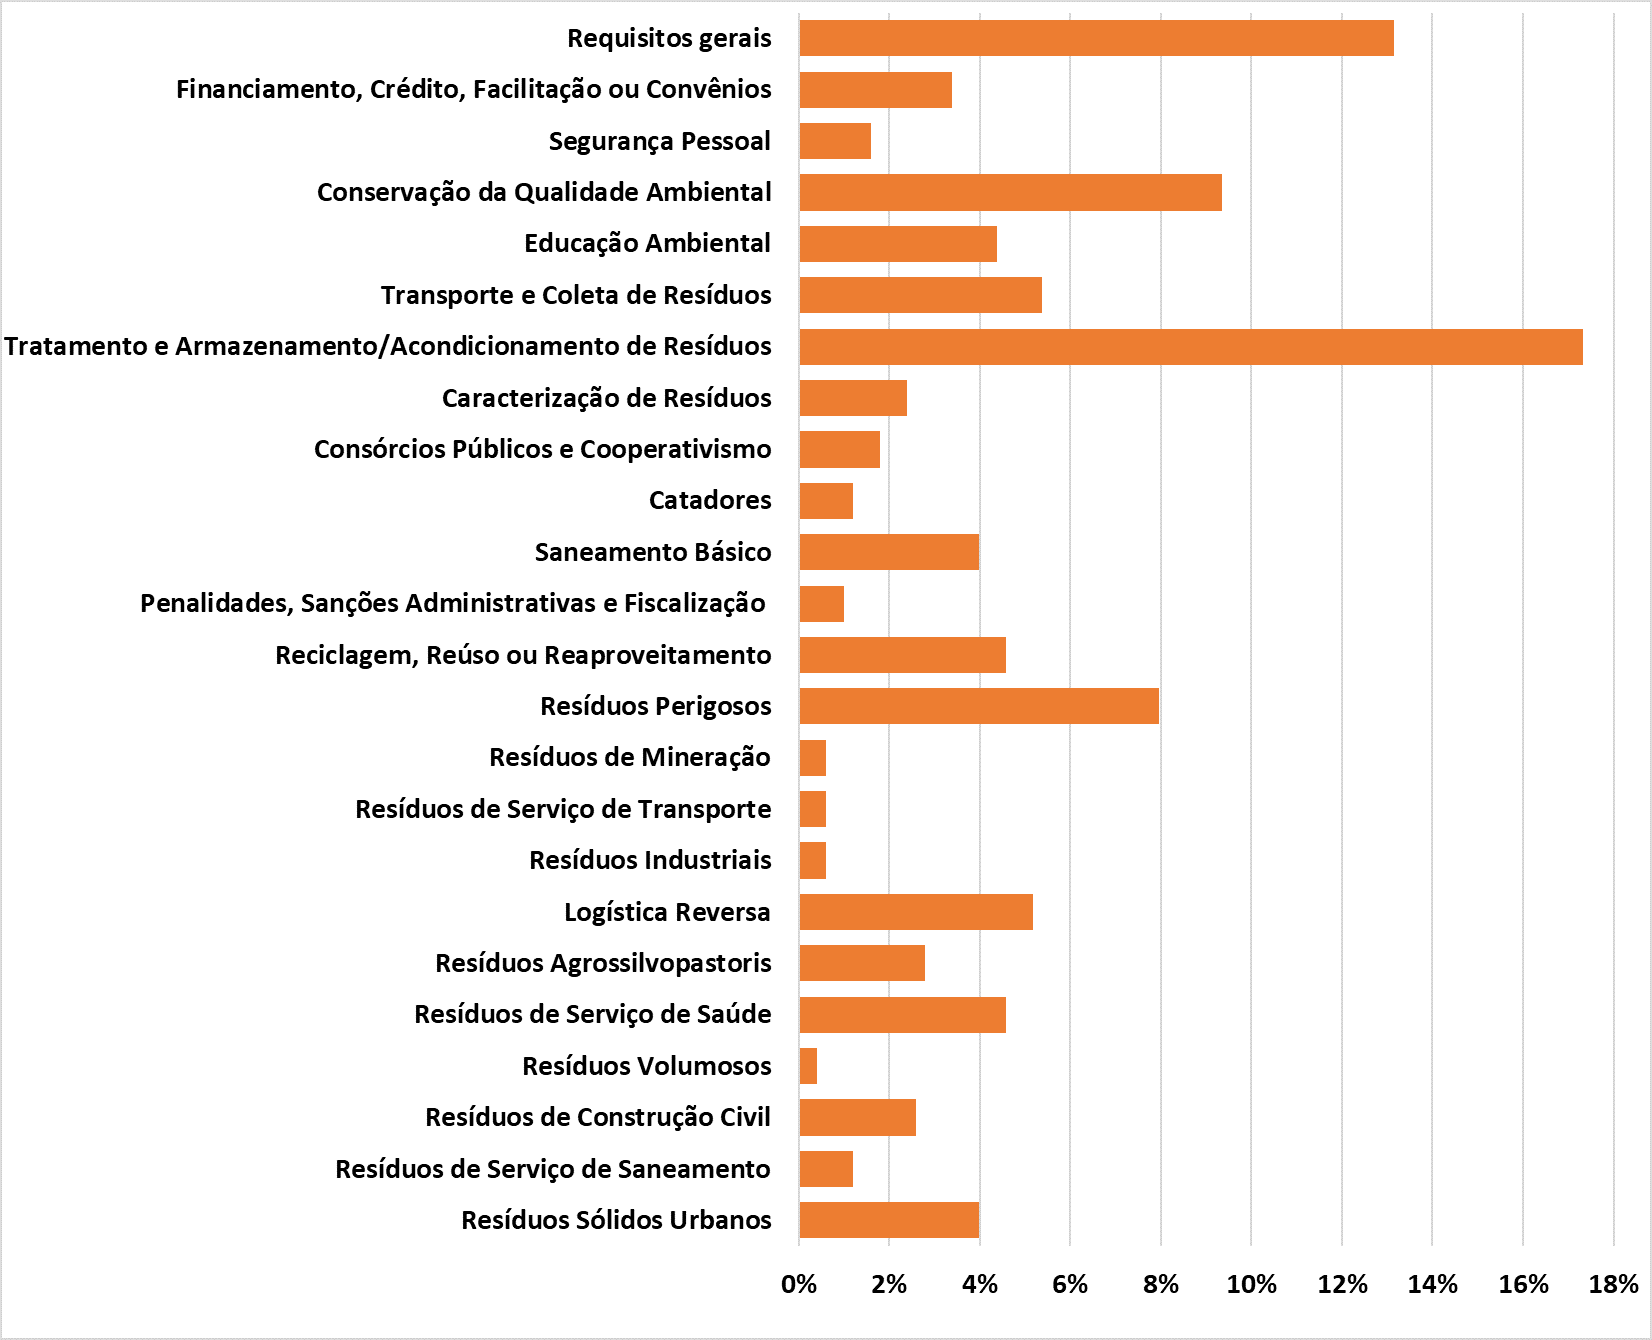
\includegraphics[width=\linewidth]{produtos/produm/distribuicaolegislacao}
		\caption{Distribuição de legislações e normas existentes por temas da gestão dos Resíduos Sólidos}
		\label{fig:distribuicaolegislacao}
	\end{figure}
	
	
	Observando a \autoref{fig:distribuicaolegislacao}, é possível verificar que a maioria das leis existentes é aplicada ao tema do tratamento e armazenamento/acondicionamento dos resíduos (17,3\% do total).
	
	Os resíduos perigosos, por sua vez, foram objeto principal de ações legisladoras, em maior parte, do governo federal. Não há, apesar do considerável número de leis de outras esferas da administração pública, nenhuma lei sobre esse tema na esfera pública municipal.
	
	Resíduos volumosos demandam grandes gastos de verbas públicas. Foi compilada apenas uma lei sobre a gestão de volumosos, municipal, que versa sobre a autorização de extrair e coletar podas de árvores volumosas ou não. Note-se que, apesar dos custos associados à gestão desse tipo de resíduos, não há nenhuma legislação específica sobre como realizar o gerenciamento de móveis, equipamentos domésticos, veículos inutilizados, entre outros.
	
	A fiscalização, juntamente com temas de sanções administrativas e penalidades, por sua vez, foi contemplada com cinco legislações em âmbito nacional e estadual e municipal, sendo apenas uma prescrita por Monteiro.
	
	Duas das legislações sobre fiscalização, uma federal e outra estadual, respectivamente, o Decreto federal Decreto 6.514/2008 e a resolução da secretaria de meio ambiente do estado de São Paulo 114/2010, versam sobre o gerenciamento de resíduos sólidos de um modo geral, com claras exigências em relação à conservação da qualidade ambiental. O único dispositivo legal municipal sobre a fiscalização, o Decreto municipal 753/1998, versa especificamente sobre a limpeza de ambientes públicos. Não há, na esfera da administração pública municipal, dispositivos legais específicos para a fiscalização de transporte, coleta, destinação final, gerenciamento de resíduos perigosos, educação ambiental, entre outros temas relevantes à gestão dos resíduos sólidos. 
	
	O tema referente à participação de catadores também foi contemplado com poucas legislações, sendo uma federal, duas estaduais e três, municipais, as quais equivalem a 1,2\% do total de leis e normas. Dentre as legislações municipais e estaduais, não há nenhuma que especifique a forma com que deve ocorrer a inclusão social e participação de catadores, o que poderia servir para detalhar assuntos abordados de forma geral pelo Programa Pró-Catador, do Decreto federal 7405/2010.
	
	A maior parte das leis e normas sobre gerenciamento de RSU foram elaboradas em nível estadual e municipal.  Diferentemente do que ocorre com os RSU, os resíduos de serviço de saneamento são quase totalmente regrados por meio de instrumentos legais e normativos em nível de federação. Os resíduos de serviços de saúde, agrossilvopastoris possuem instrumentos regulamentadores de todas as esferas de governo.
	
	Os resíduos da construção civil possuem maioria de legislações municipais. Ressalta-se a lei municipal 865/91, que versa sobre a doação de materiais de construção a famílias de baixa renda. Essa lei, caso seja implementada, poderá, ao mesmo tempo, diminuir os custos de disposição dos materiais descartados, ainda em condições de uso, e promover ganhos sociais.
	
	Os resíduos de logística reversa (pilhas e baterias, pneus, óleos lubrificantes e suas embalagens, lâmpadas fluorescentes e produtos eletroeletrônicos e seus componentes) não foram contemplados por nenhuma legislação municipal. A maior parte dos regramentos para a logística reversa foi feita pelo governo federal. Nesse contexto, percebe-se que não há detalhamentos em nível local sobre como o sistema logístico deverá ocorrer. Resíduos industriais não foram contemplados por nenhuma legislação municipal ou estadual, existindo somente em âmbito federal.
	
	De acordo com a administração municipal, serviços de transporte, tais como o transporte escolar, são indispensáveis à dinâmica econômica e cultural de Monteiro Lobato. No entanto, os resíduos gerados nesse setor, ainda não possuem regramentos específicos de gerenciamento, elaborados por ações legisladoras em nível regional ou local.
	
	Resíduos gerados por mineração não possuem leis estaduais. Além das exigências legais em nível federal, o município possui, em nível local, exigências sobre a prática de mineração e seus rejeitos gerados.
	
	
% ------
%\addcontentsline{toc}{section}{Referências}
\bibliography{pmgirs-bib}\thispagestyle{headfootimage}
% ------


\apendices
\BeginNoToc
\thispagestyle{headfootimage}




\titleformat{\subsection}
{\Large\bfseries\scshape\raggedright}
{\thesubsection}{1em}
{}
\titleformat{\subsubsection}
{\Large\bfseries\scshape\raggedright}
{\thesubsubsection}{1em}
{}
\titlespacing*{\section}{0pt}{*2}{*2}
\titlespacing*{\subsection}{0pt}{*0.5}{*0}
\titlespacing*{\subsubsection}{1cm}{*0}{*0}

\newenvironment{subapend}{%
	\begin{adjustwidth}{0.1\textwidth}{0cm}
	}{
	\end{adjustwidth}
}
\newenvironment{subsubapend}{%
	\begin{adjustwidth}{0.1\textwidth}{0cm}
	}{
	\end{adjustwidth}
}

\chapter{Classificação de exigências legais e normativas}

A seguir, as exigências legais aplicáveis à gestão municipal de resíduos sólidos em Monteiro Lobato serão classificadas em temas e em esfera de governo, segundo seu conteúdo e/ou a descrição da lei.

\section{Resíduos Sólidos Urbanos}

\begin{subapend}
	\subsection{Federal}
	\begin{subsubapend}
		\subsubsection{Lei 11.445/2007}
		Sobre saneamento básico (possui conteúdo sobre RSU).
		\subsubsection{NBR 1.299/1993}
		Sobre a coleta, varrição e acondicionamento de resíduos sólidos urbanos – Terminologia.
		\subsubsection{NBR 8.419/1996}
		Sobre procedimentos para a apresentação de projetos de aterro sanitário de resíduos sólidos urbanos.
		\subsubsection{NBR 12.980/1993}
		Esta Norma define os termos utilizados na coleta, varrição e acondicionamento de resíduos sólidos urbanos.
		\subsubsection{NBR 15.911/2011}
		Sobre o contentor móvel de plásticoParte 2: Contentor de duas rodas, com capacidade de 120 L, 240 L e 360 L, destinado à coleta de resíduos sólidos urbanos (RSU) e de saúde (RSS) por coletor compactador.
	\end{subsubapend}
\end{subapend}


\begin{subapend}
	\subsection{Estadual}
	\begin{subsubapend}
		\subsubsection{Constituição Estadual}
		Estabelece políticas, ações e deveres de saneamento básico.
		\subsubsection{Lei complementar nº 1.025/200}
		Transforma a Comissão de Serviços Públicos de Energia – CSPE em Agência Reguladora de Saneamento e Energia do Estado de São Paulo – ARSESP, dispõe sobre os serviços públicos de saneamento básico e de gás canalizado no Estado, e dá outras providências.
		\subsubsection{Lei nº 7.750/1992}
		Sobre a política estadual de saneamento.
		\subsubsection{Lei nº 10.763/2001}
		Dispõe sobre medidas a serem adotadas na prevenção e controle às inundações. Obs: Há menções do lixo urbano como uma das principais causas de inundações.
		\subsubsection{Lei 10.888/2001}
		Sobre o descarte final de produtos potencialmente perigosos do resíduo urbano que contenham metais pesados.
		\subsubsection{Decreto 55.565/2010}
		Sobre a prestação de serviços públicos de saneamento básico relativos à limpeza urbana e ao manejo de resíduos sólidos urbanos no estado de São Paulo e dá providências correlatas.
		\subsubsection{Norma Cetesb P4.241 (Sem Data)}
		Norma para apresentação de projetos de aterros sanitários de resíduos urbanos.
		\subsubsection{Resolução SSE/SMA 49/200}
		Cria Grupo de Trabalho para propor um programa estadual de aproveitamento energético de resíduos sólidos urbanos e outros rejeitos da atividade econômica.
	\end{subsubapend}
\end{subapend}

\begin{subapend}
	\subsection{Municipal}
	\begin{subsubapend}
		\subsubsection{Lei Orgânica do Município de Monteiro Lobato. Promulgada em 1990 e atualizada em 2007.}
		Art. 98
		Estabelece procedimentos para a implantação de Planos de obras e serviços municipais.
		\subsubsection{Lei 1.296/05}
		Locação imóvel destinado ao depósito de Merenda Escolar
		\subsubsection{Lei 1.350/07}
		Locação imóvel destinado ao Depósito de Merenda Escola. 
		\subsubsection{Lei 1.417/09}
		Locação de imóvel destinado a marcenaria e depósito do Setor de Serviços Urbanos.
		\subsubsection{Lei 1.447/09}
		Autoriza a administração municipal a podar, extrair ou Substituir Árvores condenadas ou em risco de queda, defronte a imóveis particulares, sem solicitação ou autorização do proprietário.
		\subsubsection{Decreto 99/1974}
		O município não cobrará taxas por serviços de limpeza em áreas urbanas durante período especificado. Importante para saber que, historicamente, o município não possui tradição de onerar o munícipe pelos serviços prestados.
		\subsubsection{Decreto 968/2006}
		Define os valores de créditos suplementares para secretarias, fundo municipal de saúde, fundo municipal de assistência social, serviços municipais urbanos e serviços de estrada de rodagem.
	\end{subsubapend}
\end{subapend}

\section{Resíduos de Serviços de Saneamento}

\begin{subapend}
	\subsection{Federal}
	\begin{subsubapend}
		\subsubsection{Resolução 375/2006}
		Define critérios e procedimentos, para o uso agrícola de lodos de esgoto gerados em estações de tratamento de esgoto sanitário e seus produtos derivados, e dá outras providências. Retificada pela Resolução nº 380 de 31 de outubro de 2006.
		\subsubsection{Resolução Conama 380/200}
		Retifica a Resolução CONAMA nº 375 de 29 de agosto de 2006 - Define critérios e procedimentos, para o uso agrícola de lodos de esgoto gerados em estações de tratamento de esgoto sanitário e seus produtos derivados, e dá outras providências.
		\subsubsection{Resolução Conama 410/2009}
		Prorroga o prazo para complementação das condições e padrões de lançamento de efluentes, previsto no art. 44 da Resolução nº 357, de 17 de março de 2005, e no Art. 3º da Resolução nº 397, de 03 de abril de 2008.
		\subsubsection{NBR 7.166/1992}
		Conexão internacional de descarga de resíduos sanitários - Formato e dimensões.
		\subsubsection{Lei nº 2.627/1954}
		Sobre a criação do Departamento de águas e esgoto do estado de São Paulo
	\end{subsubapend}
\end{subapend}

\begin{subapend}
	\subsection{Municipal}
	\begin{subsubapend}
		\subsubsection{Lei 864/91}
		Firma convênio com a Companhia de Saneamento Básico do Estado de São Paulo - SABESP, para obras de implantação do sistema de coleta, tratamento e disposição final de esgotos sanitários a ser executado no Município.
	\end{subsubapend}
\end{subapend}



\section{Resíduos de Construção Civil}
\subsection{Federal}
\begin{subapend}
	\begin{subsubapend}
		\subsubsection{Resolução Conama 307/2002}
		Sobre gerenciamento de RCC, alterada pelas resoluções 348/2004, 431/2011, 448/2012, 469/2015.
		\subsubsection{NBR 15.112/2004}
		Sobre os resíduos da construção civil e resíduos volumosos; ATTs; diretrizes para projeto, implantação e operação.
		\subsubsection{NBR 15.113/2004}
		Sobre RCC e inertes - aterros.
		\subsubsection{NBR 15.114/2004}
		Sobre RCC - áreas de reciclagem.
		\subsubsection{NBR 15.115/2004}
		Sobre RCC e agregados reciclados.
		\subsubsection{NBR 15.116/2004}
		Sobre RCC e uso de agregados em construções e pavimentações.
		\subsubsection{NR 18}
		Sobre as Condições e Meio Ambiente de Trabalho na Indústria da Construção. Possui conteúdo sobre exigências e procedimentos para armazenamento de entulho.
	\end{subsubapend}
\end{subapend}


\begin{subapend}
	\subsection{Estadual}
	\begin{subsubapend}
		\subsubsection{Lei nº 119/1973}
		Sobre a constituição da Sabesp.
		\subsubsection{Resolução da SMA 81/2014}
		Estabelece diretrizes para implementação do Módulo Construção Civil do Sistema Estadual de Gerenciamento Online de Resíduos Sólidos – SIGOR, e dá providências correlatas.
		\subsection{Municipal}
		\subsubsection{Lei Orgânica do Município de Monteiro Lobato. Promulgada em 1990 e atualizada em 2007.}
		\subsubsection{Art. 98}
		Estabelece procedimentos para a implantação de Planos de obras e serviços municipais.
		\subsubsection{Lei 865/91}
		Dispõe sobre doação de materiais de construção a famílias de baixa renda.
		\subsubsection{Lei 1.442/09}
		Dispõe sobre Estudo e Relatório de Impacto Ambiental nos projetos de edificações.
		\subsubsection{Lei 1.541/13}
		Sobre a obrigatoriedade do uso de tapumes de folhas ou chapas de ferro ou alumínio em obras de construções ou reformas realizadas pelos Poderes Executivo e Legislativo e pelos órgãos estaduais.
	\end{subsubapend}
\end{subapend}



\section{Resíduos Volumosos}
\begin{subapend}
	\subsection{Federal}
	\begin{subsubapend}
		\subsubsection{NBR 15.112/2004}
		Resíduos da construção civil e resíduos volumosos; ATTs; diretrizes para projeto, implantação e operação.
	\end{subsubapend}
\end{subapend}

\begin{subapend}
	\subsection{Municipal}
	\begin{subsubapend}
		\subsubsection{Lei 1.447/09}
		Autoriza a administração Municipal a Podar,Extrair ou Substituir Árvores condenadas ou em risco de queda, defronte a imóveis particulares, sem solicitação ou autorização do proprietário.
	\end{subsubapend}
\end{subapend}



\section{Resíduos de Serviço de Saúde}
\begin{subapend}
\subsection{Federal}	
	\begin{subsubapend}
		
		\subsubsection{Lei 9782/1999}
		Dispõe sobre os resíduos sob responsabilidade da Vigilância Sanitária. Incumbe à Agência, respeitada a legislação em vigor, regulamentar, controlar e fiscalizar os produtos e serviços que envolvam risco à saúde pública como alimentos, inclusive bebidas, águas envasadas, seus insumos, suas embalagens, aditivos alimentares, limites de contaminantes orgânicos, resíduos de agrotóxicos e de medicamentos veterinários.
		\subsubsection{Resolução Conama 06/1991}
		Dispõe sobre tratamento de RSS, resíduos de aeroportos e portos - alterada posteriormente.
		\subsubsection{Resolução Conama 358/2005}
		Sobre tratamento e disposição final de RSS. Revoga as resoluções 5/93 e 283/2001.
		\subsubsection{Resolução RDC ANVISA 305/2002}
		Sobre tratamento de RSS e materiais descartados ou acondicionados.
		\subsubsection{Resolução RDC ANVISA 306/2004}
		Sobre o gerenciamento de RSS - revoga a RDC 33/2003.
		\subsubsection{NBR 12.807/1993}
		Sobre os resíduos de serviços de saúde – Terminologia.
		\subsubsection{NBR 12.808/2016}
		Sobre os resíduos de serviço de saúde – Classificação.
		\subsubsection{NBR 12.809/2013}
		Esta Norma estabelece os procedimentos necessários ao gerenciamento intra estabelecimento de resíduos de serviços de saúde os quais, por seus riscos biológicos e químicos, exigem formas de manejo específicos, a fim de garantir condições de higiene, segurança e proteção à saúde e ao meio ambiente.
		\subsubsection{NBR 12.810/2016.}
		Sobre o gerenciamento de RSS fora do ambiente gerador.
		\subsubsection{NBR 14.652/2013}
		Sobre coleta e transporte de RSS.
		\subsubsection{NBR 15.911/2011}
		Contentor móvel de plástico. Parte 2: Contentor de duas rodas, com capacidade de 120 L, 240 L e 360 L, destinado à coleta de resíduos sólidos urbanos (RSU) e de saúde (RSS) por coletor compactador.
	\end{subsubapend}
\end{subapend}

\begin{subapend}
	\subsection{Estadual}
	\begin{subsubapend}
		\subsubsection{Decisão Cetesb nº. 3-E/2004}
		Homologa a Norma Técnica P4.262 - Gerenciamento de Resíduos Químicos Provenientes de Estabelecimentos de Serviços de Saúde - Procedimento (dezembro/2003).
		\subsubsection{Decisão Cetesb nº. 224/2007/E}
		Dispõe sobre a homologação da revisão da Norma Técnica P.4.262 - Gerenciamento de Resíduos Químicos provenientes de Estabelecimentos de Serviços de Saúde - Procedimento - agosto/2007 - e dá outras providências.
		\subsubsection{Norma Cetesb P4.262/2007}
		Gerenciamento de resíduos químicos provenientes de estabelecimentos de serviço de saúde - procedimento.
		\subsubsection{Norma Cetesb E15.010/2011}
		Sistemas de tratamento térmico sem combustão de resíduos de serviços de saúde contaminados biologicamente: procedimento.
		\subsubsection{Norma Cetesb E15.011/2007}
		Sistema de Incineração de Resíduos de Serviços de Saúde - Procedimento.
		\subsubsection{Portaria da Secretaria Estadual de Meio Ambiente  CVS nº 21/2008}
		Normas para gerenciamento de RSS.
		\subsubsection{SS/SMA/SJDC-SP 1/2004}
		Estabelece classificação, as diretrizes básicas e o regulamento técnico sobre Resíduos de Serviços de Saúde Animal - R.S.S.A
		\subsubsection{Resolução da SMA 22/2007}
		Estabelece que os resíduos citados pela Conama 358/2005 devem ter estabelecimentos de tratamento licenciados pela Cetesb.
		\subsubsection{Resolução da SMA 33/2005}
		Dispõe sobre procedimentos para o gerenciamento e licenciamento ambiental de sistemas de tratamento e disposição final de resíduos de serviços de saúde humana e animal no Estado de São Paulo. Revoga a 31/2003.
		\subsubsection{Resolução da SMA 103/2012}
		Dispõe sobre a fiscalização do gerenciamento de resíduos de serviços de saúde.
	\end{subsubapend}
\end{subapend}


\begin{subapend}
	\subsection{Municipal}
	\begin{subsubapend}
		\subsubsection{Lei Orgânica do Município de Monteiro Lobato. Promulgada em 1990 e atualizada em 2007.}
		\subsubsection{Art. 98}
		Estabelece procedimentos para a implantação de Planos de obras e serviços municipais.
		\subsubsection{Decreto 968/2006}
		Define os valores de créditos suplementares para secretarias, fundo municipal de saúde, fundo municipal de assistência social, serviços municipais urbanos e serviços de estrada de rodagem.
	\end{subsubapend}
\end{subapend}


 
\section{Resíduos Agrossilvopastoris}
\begin{subapend}
	\subsection{Federal}
	\begin{subsubapend}
		\subsubsection{Lei 7802/1989}
		Sobre a pesquisa, a experimentação, a produção, a embalagem e rotulagem, o transporte, o armazenamento, a comercialização, a propaganda comercial, a utilização, a importação, a exportação, o destino final dos resíduos e embalagens, o registro, a classificação, o controle, a inspeção e a fiscalização de agrotóxicos, seus componentes e afins, e dá outras providências.
		\subsubsection{Lei 9782/1999}
		Dispõe sobre os resíduos sob responsabilidade da Vigilância Sanitária. Incumbe à Agência, respeitada a legislação em vigor, regulamentar, controlar e fiscalizar os produtos e serviços que envolvam risco à saúde pública como alimentos, inclusive bebidas, águas envasadas, seus insumos, suas embalagens, aditivos alimentares, limites de contaminantes orgânicos, resíduos de agrotóxicos e de medicamentos veterinários.
		\subsubsection{Lei 9974/2000}
		Altera a Lei no 7.802/1989, que dispõe sobre a pesquisa, a experimentação, a produção, a embalagem e rotulagem, o transporte, o armazenamento, a comercialização, a propaganda comercial, a utilização, a importação, a exportação, o destino final dos resíduos e embalagens, o registro, a classificação, o controle, a inspeção e a fiscalização de agrotóxicos, seus componentes e afins, e dá outras providências.
		\subsubsection{Decreto 4074/2002}
		Regulamenta a lei 7802/1989 e a lei 3550/2000.
		\subsubsection{NBR 13.227/2017}
		Sobre agrotóxicos e afins - Determinação de resíduo não volátil
		\subsubsection{NBR 13.237/2017}
		Esta Norma especifica um método de ensaio para determinação do resíduo por peneiramento úmido de produtos agrotóxicos e afins. 
		\subsubsection{NBR 14.719/2001}
		Estabelece os procedimentos para a destinação final das embalagens rígidas, usadas, vazias, adequadamente lavadas de acordo com a NBR 13968, que contiveram formulações de agrotóxicos miscíveis ou dispersíveis em água.
		\subsection{Estadual}
		\subsubsection{Lei nº 10.547/2000}
		Define procedimentos, proibições, estabelece regras de execução e medidas de precaução a serem obedecidas quando do emprego do fogo em práticas agrícolas, pastoris e florestais. Obs: há sugestões de uso de resíduos agrícola nessas práticas.
		\subsubsection{Decisão Cetesb nº. 88/2012}
		Dispõe sobre a prorrogação do prazo fixado para que as pessoas físicas e/ou jurídicas que possuam estoques de agrotóxicos obsoletos, em especial os considerados POP's, declarem a situação de seu armazenamento e acondicionamento, com vistas à elaboração de projeto para a eliminação desses resíduos no Estado de São Paulo, e dá outras providências.
		\subsubsection{Decisão Cetesb nº. 273/2010}
		Dispõe sobre a Homologação da Norma Técnica de Efluentes e Lodos Fluidos de Indústrias Cítricas - Critérios e Procedimentos para aplicação no solo agrícola.
		\subsubsection{Decisão Cetesb nº. 388/2010}
		Aprova premissas e diretrizes para a aplicação de resíduos e efluentes em solo agrícola no Estado de São Paulo.
		\subsubsection{Norma Cetesb P4.231/2006}
		Sobre a vinhaça - Critérios e Procedimentos para Aplicação no Solo Agrícola Norma Cetesb P4.262 (2004) Dispõe sobre procedimentos para utilização de resíduos em fornos de produção clinquer (processo E/341/2003) – dezembro de 2003.
		\subsubsection{Resolução da SMA 50/2007}
		Define as diretrizes para a adequação ambiental de imóveis rurais com vistas à participação no Projeto Mina D’Água. Obs: possui exigências em relação aos resíduos sólidos.
	\end{subsubapend}
\end{subapend}

\begin{subapend}
\subsection{Municipal}	
	\begin{subsubapend}
		\subsubsection{Lei Orgânica (Resolução 1/2007)}
		Cap. XVIII - o-) “ao uso e armazenamento dos agrotóxicos, seus componentes e afins, bem como, a coleta e ao controle diferenciado do lixo produzido por estes produtos”;   
	\end{subsubapend}
\end{subapend}

\section{Resíduos de Logística Reversa}

\begin{subapend}
	\subsection{Federal}
	\begin{subsubapend}
		\subsubsection{Lei 7802/1989}
		Sobre a pesquisa, a experimentação, a produção, a embalagem e rotulagem, o transporte, o armazenamento, a comercialização, a propaganda comercial, a utilização, a importação, a exportação, o destino final dos resíduos e embalagens, o registro, a classificação, o controle, a inspeção e a fiscalização de agrotóxicos, seus componentes e afins, e dá outras providências.
		\subsubsection{Lei 9177/2017}
		Regulamenta o art. 33 da Lei nº 12.305, de 2 de agosto de 2010, que institui a Política Nacional de Resíduos Sólidos, e complementa os art. 16 e art. 17 do Decreto nº 7.404, de 23 de dezembro de 2010 e dá outras providências.
		\subsubsection{Lei 9974/2000}
		Altera a Lei no 7.802/1989, que dispõe sobre a pesquisa, a experimentação, a produção, a embalagem e rotulagem, o transporte, o armazenamento, a comercialização, a propaganda comercial, a utilização, a importação, a exportação, o destino final dos resíduos e embalagens, o registro, a classificação, o controle, a inspeção e a fiscalização de agrotóxicos, seus componentes e afins, e dá outras providências.
		\subsubsection{Decreto 4074/2002}
		Regulamenta a lei 7802/1989 e a lei 3550/2000.
		\subsubsection{Resolução Conama 362/2005}
		Sobre coleta e destinação de óleo usado ou contaminado - revoga a Resolução 9/1993 e foi alterada pela Resolução 450/2012.
		\subsubsection{Resolução Conama 362/2005.}
		Dispõe sobre o recolhimento, coleta e destinação final de óleo lubrificante usado ou contaminado.
		\subsubsection{Resolução Conama 401/2008}
		Sobre gerenciamento e limites de metais em pilhas e baterias que contêm chumbo, mercúrio e cádmio - revoga a 257/1999.
		\subsubsection{Resolução Conama 416/2009}
		Dispõe sobre a prevenção à degradação ambiental causada por pneus inservíveis e sua destinação ambientalmente adequada (Revoga a resolução 258/1999).
		\subsubsection{Resolução Conama 424/2010}
		Altera um parágrafo da Resolução 401/2008, sobre importação de pilhas e baterias.
		\subsubsection{Resolução Conama 450/2012}
		Altera os arts. 9º, 16, 19, 20, 21 e 22, e acrescenta o art. 24-A à Resolução nº 362/2005, que dispõe sobre recolhimento, coleta e destinação final de óleo lubrificante usado ou contaminado.
		\subsubsection{Resolução Conama 465/2014}
		Sobre os requisitos e critérios técnicos mínimos necessários para o licenciamento ambiental de estabelecimentos destinados ao recebimento de embalagens de agrotóxicos e afins, vazias ou contendo resíduos. Revoga a Resolução nº 334/2003.
		\subsubsection{NBR 13.227/2017}
		Agrotóxicos e afins - Determinação de resíduo não volátil
		\subsubsection{NBR 13.237/2017}
		Esta Norma especifica um método de ensaio para determinação do resíduo por peneiramento úmido de produtos agrotóxicos e afins. 
		\subsubsection{NBR 14.719/2001}
		Estabelece os procedimentos para a destinação final das embalagens rígidas, usadas, vazias, adequadamente lavadas de acordo com a NBR 13968, que contiveram formulações de agrotóxicos miscíveis ou dispersíveis em água.
		\subsubsection{NBR 15.833/2010}
		Esta Norma prescreve os procedimentos para o transporte, armazenamento e desmonte com reutilização, recuperação dos materiais recicláveis e destinação final de resíduos dos aparelhos de refrigeração.
		\subsubsection{NBR 16.156/2013}
		Esta Norma estabelece requisitos para proteção ao meio ambiente e para o controle dos riscos de segurança e saúde no trabalho na atividade de manufatura reversa de resíduos eletroeletrônicos.
		\subsubsection{IN do IBAMA 01/2010}
		Procedimentos do Ibama e sobre fabricação, importação, coleta e destinação final de pneus.
		\subsubsection{IN do IBAMA 08/2012}
		Procedimentos e destinação final de pilhas e baterias.
	\end{subsubapend}
\end{subapend}

\begin{subapend}
	\subsection{Estadual}
	\begin{subsubapend}
		\subsubsection{Lei nº 12.288/2006}
		Dispõe sobre a eliminação controlada dos PCBs e dos seus resíduos, a descontaminação de transformadores, capacitores e demais equipamentos elétricos que contenham PCBs, e dá providências correlatas.
		\subsubsection{Lei 13.576/2009}
		Sobre a destinação, reciclagem e gerenciamento do lixo tecnológico.
		\subsubsection{Lei nº 14.186/2010}
		Dispõe sobre a coleta, o recolhimento e o destino final das embalagens plásticas de óleos lubrificantes, e dá outras providências correlatas.
		\subsubsection{Lei nº 15.276/2014}
		Dispõe sobre a destinação de veículos em fim de vida útil e dá outras providências.
		\subsubsection{Decreto nº 60.150/2014}
		Regulamenta a Lei nº 15.276, de 2014, que dispõe sobre a destinação de veículos em fim de vida útil.
		\subsubsection{Decisão Cetesb nº. 88/2012}
		Dispõe sobre a prorrogação do prazo fixado para que as pessoas físicas e/ou jurídicas que possuam estoques de agrotóxicos obsoletos, em especial os considerados POP's, declarem a situação de seu armazenamento e acondicionamento, com vistas à elaboração de projeto para a eliminação desses resíduos no Estado de São Paulo, e dá outras providências.
		\subsubsection{Resolução da SMA - SP 11/2012}
		Trata dos programas de responsabilidade pós-consumo no setor da telefonia móvel celular.
		\subsubsection{Resolução da SMA 115/2013}
		Trata do estabelecimento de programas de responsabilidade pós-consumo para os medicamentos domiciliares, vencidos ou em desuso.
	\end{subsubapend}
\end{subapend}	


\section{Resíduos Industriais}
\begin{subapend}
	\subsection{Federal}
	\begin{subsubapend}
		\subsubsection{NR 25}
		Sobre os Resíduos Industriais.
	\end{subsubapend}
\end{subapend}

\begin{subapend}
	\subsection{Estadual}
	\begin{subsubapend}
		\subsubsection{Norma Cetesb L5.510/1982}
		Lixiviação de resíduos industriais: Método de Ensaio.
		\subsubsection{Norma Cetesb L10.101/1988}
		Sobre os resíduos sólidos industriais – tratamento no solo: Procedimento.
	\end{subsubapend}
\end{subapend}

\section{Resíduos de Serviços de Transporte}
\begin{subapend}
	\subsection{Federal}
	\begin{subsubapend}
		\subsubsection{Resolução Conama 02/1991}
		Sobre os procedimentos para o tratamento de cargas deterioradas e sobre a competência pela solução e pelos custos de avaliação, monitoramento, controle e gerenciamento dos resíduos gerados pelas cargas.
		\subsubsection{Resolução Conama 06/1991}
		Dispões sobre tratamento de RSS, resíduos de aeroportos e portos - alterada posteriormente.
		\subsubsection{Resolução RDC ANVISA 56/2008}
		Dispõe sobre o Regulamento Técnico de Boas Práticas Sanitárias no Gerenciamento de Resíduos Sólidos nas áreas de Portos, Aeroportos, Passagens de Fronteiras e Re­cintos Alfandegados.
	\end{subsubapend}
\end{subapend}

\section{Resíduos de Mineração}

\begin{subapend}
	\subsection{Federal}
	\begin{subsubapend}
		\subsubsection{NBR 13.029/2017}
		Esta Norma especifica os requisItos mínimos para a elaboração e apresentação de projeto de pilha para disposição de estéril gerado por lavra de mina a céu aberto ou de mina subterrânea, visando atender às condições de segurança, operacionalidade, economia e desativação, minimizando os impactos ao meio ambiente.
		\subsubsection{NR 22}
		Sobre a Segurança e Saúde Ocupacional na Mineração. Aplicável no monitoramento das ações relacionadas aos resíduos de mineração.
	\end{subsubapend}
\end{subapend}


\begin{subapend}
	\subsection{Municipal}
	\begin{subsubapend}
		\subsubsection{Lei Orgânica Art. 179}
		Exige licença para atividades de mineração e obtenção de consolidados rochosos do solo, particulados ou não.
	\end{subsubapend}
\end{subapend}

\section{Resíduos Perigosos}

\begin{subapend}
	\subsection{Federal}
	\begin{subsubapend}
		
		\subsubsection{Lei 9966/2000}
		Dispõe sobre a prevenção, o controle e a fiscalização da poluição causada por lançamento de óleo e outras substâncias nocivas ou perigosas em águas sob jurisdição nacional e dá outras providências.
		\subsubsection{Decreto 875/1993}
		Sobre a Convenção de Brasileira, de 1989, sobre o controle de movimentos transfronteiriços de resíduos perigosos e seu depósito.
		\subsubsection{Decreto no 2.063/1983}
		Estabelece multas por infrações ligadas ao transporte de produtos perigosos.
		\subsubsection{Decreto 4.136/2002}
		Regulamenta a lei 9966/2000.
		\subsubsection{Portaria Ministerial 261/1989}
		Sobre o transporte rodoviário de produtos perigosos
		\subsubsection{ANTT: Resolução 420/2004}
		Sobre as instruções complementares do transporte terrestre de produtos perigosos e substituiu Portarias publicadas pela ANTT entre 1989 e 2001. A Resolução foi alterada pela Resolução ANTT no 701/2004
		\subsubsection{Resolução Conama 023/1996}
		Regulamenta a importação e uso de resíduos perigosos. Revoga a Resolução nº 37, de 1994. Alterada pelas Resoluções nº 235, de 1998, e nº 244, de 1998. Revogada pela Resolução nº 452, de 2012.
		\subsubsection{Resolução Conama 228/1997}
		Dispõe sobre a importação de desperdícios e resíduos de acumuladores elétricos de chumbo.
		\subsubsection{Resolução Conama 252/2012}
		Sobre os procedimentos de controle da importação de resíduos conforme as normas adotadas pela Convenção da Basileia sobre o controle de movimentos transfronteiriços de resíduos perigosos e seu depósito. Revogou todas as Resoluções do CONAMA as quais tratavam da matéria até então.
		\subsubsection{Resolução Conama 420/2009}
		Dispõe sobre critérios e valores orientadores de qualidade do solo quanto à presença de substâncias químicas e estabelece diretrizes para o gerenciamento ambiental de áreas contaminadas por essas substâncias em decorrência de atividades antrópicas.
		\subsubsection{Resolução 452/2012}
		Sobre os procedimentos de controle da importação de resíduos, conforme as normas adotadas pela Convenção da Basiléia sobre o Controle de Movimentos Transfronteiriços de Resíduos Perigosos e seu Depósito - Revoga as Resoluções nº 08/1991, nº 23/1996, nº 235/1998 e nº 244/1998.
		\subsubsection{CP ANVISA 32/2004}
		Sobre a simbologia para resíduos perigosos.
		\subsubsection{NBR 7.500/2017}
		Sobre identificação e simbologias de resíduos perigosos.
		\subsubsection{NBR 8.418/1984}
		Sobre a presentação de projetos de aterros de resíduos industriais perigosos - Procedimento.
		\subsubsection{NBR 9.735/2006}
		Conjunto de equipamentos para emergências no transporte terrestre de produtos perigosos.
		\subsubsection{NBR 10.157/1987}
		Aterros de resíduos perigosos - Critérios para projeto, construção e operação – Procedimento.
		\subsubsection{NBR 11.175/1990}
		Sobre a incineração de resíduos sólidos perigosos - Padrões de desempenho – Procedimento.
		\subsubsection{NBR 13.853/1997}
		Sobre gerenciamento de resíduos descartáveis perfurantes e cortantes.
		\subsubsection{NBR 14.725/2014}
		Sobre os riscos à saúde e ao meio ambiente, que substâncias químicas podem apresentar.
		\subsubsection{NBR 16.725/2014}
		Sobre resíduo químico - Informações sobre segurança, saúde e meio ambiente - Ficha com dados de segurança de resíduos químicos (FDSR) e rotulagem.
		\subsubsection{NR 20}
		Sobre a Segurança e Saúde no Trabalho com Inflamáveis e Combustíveis. Aplicável sempre que esse tipo de material for manuseado.
		\subsubsection{NR 23}
		Sobre a Proteção Contra Incêndios. Aplicável sempre que houver risco de incêndio em função da característica de alguns resíduos sólidos.
		\subsubsection{IN do IBAMA 05/2012}
		Sobre transporte de resíduos perigosos.
		\subsubsection{IN do IBAMA 01/2013}
		Refere-se ao cadastro Nacional de Operadores de Resíduos Perigosos e prestação de informações sobre resíduos sólidos.
	\end{subsubapend}
\end{subapend}

\begin{subapend}
	\subsection{Estadual}
	\begin{subsubapend}
		\subsubsection{Lei 10.888/2001}
		Sobre o descarte final de produtos potencialmente perigosos do resíduo urbano que contenham metais pesados.
		\subsubsection{Lei nº 12.684/2007}
		Proíbe o uso, no Estado de São Paulo de produtos, materiais ou artefatos que contenham quaisquer tipos de amianto ou asbesto ou outros minerais que, acidentalmente, tenham fibras de amianto na sua composição. Alterada pela lei nº 16.048/2015.
		\subsubsection{Lei nº 15.303/2014}
		Institui o Programa Estadual de Incentivo ao uso de matérias–primas e insumos derivados de materiais reciclados provenientes da indústria petroquímica.
		\subsubsection{Lei nº 15.313/2014}
		Dispõe sobre a proibição do uso, armazenamento e reparo de instrumentos de medição como esfigmomanômetros e termômetros contendo mercúrio e dá outras providências.
		\subsubsection{Decreto nº 45.643/2001}
		Dispõe sobre a obrigatoriedade da aquisição pela Administração Pública Estadual de lâmpadas de maior eficiência energética e menor teor de mercúrio, por tipo e potência, e dá providências correlatas.
		\subsubsection{Decisão Cetesb nº. 3-E/2004}
		Homologa a Norma Técnica P4.262 - Gerenciamento de Resíduos Químicos Provenientes de Estabelecimentos de Serviços de Saúde - Procedimento (dezembro/2003).
		\subsubsection{Decisão Cetesb nº. 27/2008}
		Dispõe sobre a aprovação do Procedimento para Utilização de Resíduos Perigosos da Indústria Têxtil em Caldeiras, no Estado de São Paulo.
		\subsubsection{Decisão Cetesb nº. 224/2007/E}
		Dispõe sobre a homologação da revisão da Norma Técnica P.4.262 - Gerenciamento de Resíduos Químicos provenientes de Estabelecimentos de Serviços de Saúde - Procedimento - agosto/2007 - e dá outras providências.
		\subsubsection{Decisão Cetesb nº. 145/2010}
		Dispõe sobre a aprovação do Procedimento de gerenciamento de resíduos de aparas de couro e de pó de rebaixadeira oriundos do curtimento ao cromo.
		\subsubsection{Decisão Cetesb nº. 152/2007}
		Dispõe sobre procedimentos para gerenciamento de areia de fundição.
		\subsubsection{Decisão Cetesb nº. 263/2009}
		Dispõe sobre a aprovação do Roteiro para Execução de Investigação Detalhada e Elaboração de Plano de Intervenção em Postos e Sistemas Retalhistas de Combustíveis.
		\subsubsection{Norma Cetesb O1.012/1985}
		Sobre o projeto e operação de aterros industriais para resíduos perigosos: Procedimento.
		\subsubsection{Norma Cetesb P4.262/2007}
		Sobre o gerenciamento de resíduos químicos provenientes de estabelecimentos de serviço de saúde - procedimento.
		\subsubsection{Norma Cetesb E15.010/2011}
		Sistemas de tratamento térmico sem combustão de resíduos de serviços de saúde contaminados biologicamente: procedimento.
		\subsubsection{Resolução da SMA 38/2011}
		Estabelece a relação de produtos geradores de resíduos de significativo impacto ambiental, para fins do disposto no artigo 19, do Decreto Estadual nº 54645/2009, que regulamenta a Lei Estadual nº 12300/2006, e dá providências correlatas. Obs: contém exigências para o comércio de produtos farmacêuticos, cosméticos e de limpeza doméstica.
		\subsubsection{Resolução da SMA 115/2013}
		Trata do estabelecimento de programas de responsabilidade pós-consumo para os medicamentos domiciliares, vencidos ou em desuso.
	\end{subsubapend}
\end{subapend}

\section{Reciclagem, Reúso ou Reaproveitamento}

\begin{subapend}
	\subsection{Federal}
	\begin{subsubapend}
		\subsubsection{Decreto 5.940/2006}
		Institui a separação dos resíduos recicláveis descartados pelos órgãos e entidades da administração pública federal direta e indireta, na fonte geradora, e a sua destinação às cooperativas.
		\subsubsection{NBR 15.114/2004}
		Sobre RCC - áreas de reciclagem.
		\subsubsection{NBR 15.115/2004}
		Sobre RCC e agregados reciclados.
		\subsubsection{NBR 15.116/2004}
		Sobre RCC e uso de agregados em construções e pavimentações.
		\subsubsection{Lei nº 14.470/2011}
		Dispõe sobre a separação dos resíduos recicláveis descartados pelos órgãos e entidades da administração pública estadual, na forma que especifica.
	\end{subsubapend}
\end{subapend}



\begin{subapend}
	\subsection{Estadual}
	\begin{subsubapend}
		\subsubsection{Lei nº 9.338/1996}
		Institui nas escolas estaduais de 1º e 2º graus a “Semana da Gincana de Coleta de Lixo Reciclável”.
		\subsubsection{Lei nº 9.532/1997}
		Sobre a semana de coleta seletiva e reciclagem de lixo.
		\subsubsection{Lei nº 12.047/2005}
		Institui Programa Estadual de Tratamento e Reciclagem de Óleos e Gorduras de Origem Vegetal ou Animal e Uso Culinário.
		\subsubsection{Lei 13.576/2009}
		Sobre a destinação, reciclagem e gerenciamento do lixo tecnológico.
		\subsubsection{Lei nº 14.731/2012}
		Inclui evento no Calendário Oficial do Estado: "Dia dos Catadores de Lixo Reciclável", a ser comemorado, anualmente, em 20 de dezembro.
		\subsubsection{Lei nº 15.303/2014}
		Institui o Programa Estadual de Incentivo ao uso de matérias–primas e insumos derivados de materiais reciclados provenientes da indústria petroquímica.
		\subsubsection{Resolução SSE/SMA 49 /2007}
		Cria Grupo de Trabalho para propor um programa estadual de aproveitamento energético de resíduos sólidos urbanos e outros rejeitos da atividade econômica.
		\subsubsection{Resolução da SMA 79/2009}
		Estabelece diretrizes e condições para a operação e o licenciamento da atividade de tratamento térmico de resíduos sólidos em Usinas de Recuperação de Energia – URE.
		\subsubsection{Resolução da SMA 88/2013}
		Institui o Cadastro de Entidades de Catadores de Materiais Recicláveis, no âmbito do Estado de São Paulo.
		
	\end{subsubapend}
\end{subapend}


\begin{subapend}
	\subsection{Municipal}
	\begin{subsubapend}
		\subsubsection{Lei 571/83}
		Fica instituída a Feira de Artesanato no Município de Monteiro Lobato.
		\subsubsection{Lei 1.295/05}
		Locação de imóvel localizado na Rua Bernardino de Campos,nº271,destinado à Reciclagem de Lixo.
		\subsubsection{Lei 1.302/05}
		Sobre a reutilização de material reciclado,no âmbito da Administração Municipal,e dá outras providências.
		\subsubsection{Lei 1.322/06}
		Sobre a locação do imóvel destinado à Reciclagem de Lixo.
		\subsubsection{Lei 1.354/07}
		Sobre a locação de imóvel destinado à Reciclagem de Lixo.
		\subsubsection{Lei 1.392/08}
		Sobre a locação de imóvel destinado à Reciclagem de Lixo.
		\subsubsection{Lei 1.418/09}
		Sobre a locação de imóvel destinado ao Depósito de Reciclagem de Lixo.
		\subsubsection{Lei 1.541/13}
		Sobre a obrigatoriedade do uso de tapumes de folhas ou chapas de ferro ou alumínio em obras de construções ou reformas realizadas pelos Poderes Executivo e Legislativo e pelos órgãos estaduais.
		\subsubsection{Decreto 1.389/2013}
		Sobre a disponibilidade de bens “inservíveis” (por ex. 220 cadeiras estofadas) para geração de renda pelo Fundo Social pela Solidariedade do município.
	\end{subsubapend}
\end{subapend}



\section{Penalidades, Sanções Administrativas e Fiscalização}

\begin{subapend}
	\subsection{Federal}
	\begin{subsubapend}
		\subsubsection{Decreto 6.514/2008}
		Dispõe sobre as infrações e sanções administrativas ao meio ambiente, estabelece o processo administrativo federal para apuração destas infrações, e dá outras providências.
		\subsubsection{Lei 9605/1998}
		Dispõe sobre as sanções penais e administrativas derivadas de condutas e atividades lesivas ao meio ambiente, e dá outras providências.
	\end{subsubapend}
\end{subapend}



\begin{subapend}
	\subsection{Estadual}
	\begin{subsubapend}
		\subsubsection{Resolução da SMA 103/2012}
		Dispõe sobre a fiscalização do gerenciamento de resíduos de serviços de saúde.
		\subsubsection{Resolução da SMA 114/2010}
		Designa os integrantes do Grupo Técnico para elaboração e acompanhamento dos Planos Regionais de Gerenciamento de Resíduos Sólidos.
		\subsection{Municipal}
		\subsubsection{Decreto 753\\1998}
		Sobre definições de Infrações e atos lesivos à limpeza pública e suas penalidades (multas).
	\end{subsubapend}
\end{subapend}



\section{Saneamento Básico}

\begin{subapend}
	\subsection{Estadual}
	\begin{subsubapend}
		\subsubsection{Decreto 7.217/2010}
		Regulamenta a lei de saneamento básico.
		\subsubsection{Resolução Conama 05/1988}
		Dispõe sobre o licenciamento de obras de saneamento básico.
	\end{subsubapend}
\end{subapend}
\subsection{Estadual}
\begin{subapend}
	
	\begin{subsubapend}
		\subsubsection{Lei nº 7.750/1992}
		Sobre a política estadual de saneamento.
		\subsubsection{Lei nº 4.882/1985}
		Sobre o Saneamento Geral e despesas relacionadas.
		\subsubsection{Constituição Estadual}
		Estabelece políticas, ações e deveres de saneamento básico.
		\subsubsection{Lei nº 8.275/1993}
		Sobre a criação da Secretaria de Recursos Hídricos, Obras e Saneamento.
		\subsubsection{Lei nº 10.083/1998}
		Dispõe sobre o código sanitário do estado.
		\subsubsection{Lei nº 10.107/1968}
		Sobre o Fundo Estadual de Saneamento Básico.
		\subsubsection{Lei nº 11.364/2003}
		Altera a denominação da Secretaria de Estado de Recursos Hídricos, Saneamento e Obras, e autoriza o Poder Executivo a extinguir a Secretaria de Estado de Energia e dá providências correlatas.
		\subsubsection{Decreto nº 50.079/1968}
		Dispõe sobre a constituição do Centro Tecnológico de Saneamento Básico, prevista na Lei Estadual nº 10.107, de 8 de maio de 1968, e dá outras providências.
		\subsubsection{Decreto 52.455/2007}
		Aprova o regulamento da Agência Reguladora de Saneamento e Energia do Estado de São Paulo - ARSESP.
		\subsubsection{Decreto nº 52.895/2008}
		Autoriza a Secretaria de Saneamento e Energia a representar o Estado de São Paulo na celebração de convênios com Municípios paulistas, ou consórcio de Municípios, visando à elaboração de planos de saneamento básico e sua consolidação no Plano Estadual de Saneamento Básico.
		\subsubsection{Decreto 55.565/2010}
		Sobre a prestação de serviços públicos de saneamento básico relativos à limpeza urbana e ao manejo de resíduos sólidos urbanos no estado de São Paulo e dá providências correlatas.
	\end{subsubapend}
\end{subapend}

\begin{subapend}
	\subsection{Municipal}
	\begin{subsubapend}
		\subsubsection{Lei 351/69}
		Autoriza o Executivo Municipal a celebrar convênio com o Fundo Estadual de Saneamento Básico, destinado a receber auxílio do Estado para os serviços de tratamento de água do Município.
		\subsubsection{Lei 514/77}
		Autoriza o Poder Executivo a outorgar à Companhia de Saneamento Básico - Sabesp, concessão para a execução e exploração dos serviços de abastecimento de água e de coleta e destino final de esgotos sanitários no Município.
		\subsubsection{Lei 572/83}
		Fica o Executivo Municipal autorizado a celebrar convênio com a Secretaria da Saúde do Estado de São Paulo, visando a melhoria da assistência médica e sanitária da população Lobatense.
		\subsubsection{Lei 864/91}
		Firma convênio com a Companhia de Saneamento Básico do Estado de São Paulo - SABESP, para obras de implantação do sistema de coleta, tratamento e disposição final de esgotos sanitários a ser executado no Município.
		\subsubsection{Lei 1.441/09}
		Celebra convênio com o Estado de São Paulo, através da Secretaria de Saneamento e Energia, objetivando a elaboração do Plano Municipal de Saneamento Básico, e sua consolidação no Plano Estadual de Saneamento Básico, em conformidade com as diretrizes gerais instituídas pela Lei Federal nº 11.445, de 05 de janeiro de 2007.
		\subsubsection{Plano Municipal Integrado de Saneamento Básico - PLASAN123}
		Descrição do dados atuais de limpeza urbana e manejo de resíduos sólidos; Projeção da geração de resíduos, ações objetivas para o sistema de limpeza urbana e manejo de resíduos sólidos; Ações objetivas para o sistema de limpeza urbana e manejo de resíduos sólidos; Planejamento do sistema de limpeza urbana e manejo de resíduos sólidos; Indicadores de resíduos sólidos e Plano de ações de contingência e emergência de serviços de limpeza pública e manejo de resíduos sólidos urbanos.
		\subsubsection{Plano de Desenvolvimento Turístico Municipal de Monteiro Lobato}
		Resumo do plano de saneamento básico.
	\end{subsubapend}
\end{subapend}

\section{Catadores}


\begin{subapend}
	\subsection{Estadual}
	\begin{subsubapend}
		\subsubsection{Decreto 7.405/2010}
		Institui o Programa Pró-Catador;
	\end{subsubapend}
\end{subapend}

\begin{subapend}
	\subsection{Estadual}
	\begin{subsubapend}
		\subsubsection{Lei nº 14.731/2012}
		Inclui evento no Calendário Oficial do Estado: "Dia dos Catadores de Lixo Reciclável", a ser comemorado, anualmente, em 20 de dezembro.
		\subsubsection{Resolução da SMA 88/2013}
		Institui o Cadastro de Entidades de Catadores de Materiais Recicláveis, no âmbito do Estado de São Paulo.
		\subsection{Municipal}
		\subsubsection{Lei 629/86}
		Autoriza a celebração de convênio entre a União Federal, através da Secretaria Especial de Ação Comunitária da Presidência da República e a Prefeitura Municipal de Monteiro Lobato, visando a implantação de projetos comunitários.
		\subsubsection{Lei 1.650/2017}
		Institui o Plano Diretor de Monteiro Lobato. Possui diretrizes para a participação de catadores de resíduos sólidos.
		\subsubsection{Decreto 225 \ 1979}
		Comissão Municipal de Promoção Social, promove a inclusão econômica e social e organização de comunidades.
	\end{subsubapend}
\end{subapend}

\section{Consórcios Públicos e Cooperativismo}

\begin{subapend}
	\subsection{Federal}
	\begin{subsubapend}
		\subsubsection{Lei 5764/1971}
		Define a Política Nacional de Cooperativismo, institui o regime jurídico das sociedades cooperativas, e dá outras providências.
		\subsubsection{Lei 11.107/2005}
		Sobre os consórcios públicos e soluções compartilhadas de gestão.
		\subsubsection{Decreto 6.007/2007}
		Regulamenta a lei de consórcios públicos - 11107/2005.
		\subsubsection{Decreto nº 6.017/2007}
		Regulamenta a Lei nº 11.107, de 6 de abril de 2005, que dispõe sobre normas gerais de contratação de consórcios públicos.
	\end{subsubapend}
\end{subapend}

\begin{subapend}
	\subsection{Municipal}
	\begin{subsubapend}
		\subsubsection{Lei 390/70}
		Autoriza o Prefeito a celebrar convênio com municípios da região para constituição do CODIVAP (Conselho de Desenvolvimento Integrado do Vale do Paraíba.
		\subsubsection{Lei 1.088/97}
		Autoriza e estabelece as condições para o Executivo Municipal promover a participação do Município na constituição, instalação e funcionamento do Consórcio Intermunicipal para reestruturação e coordenação da gestão das atividades de obras e serviços viários nas esferas dos municípios consorciados e seus respectivos territórios, com a realização de todos os atos referentes à viabilização e efetivação das concessões de obras e serviços, com consonância com a vontade dos consorciados e com projetos globais de caráter geral encaminhados pelo Estado e União.
		\subsubsection{Lei 1.171/01}
		Autoriza a Prefeitura de Monteiro Lobato, a participar do Consórcio Intermunicipal para conservação e manutenção de vias públicas municipais.
		\subsubsection{Lei 1.563/13}
		Ratifica o Protocolo de Intenções que celebram entre si os Municípios de Santo Antônio do Pinhal, São Bento do Sapucaí, Monteiro Lobato, Tremembé e Campos do Jordão, visando à re-adequação legal do Consórcio Intermunicipal Serra da Mantiqueira - CISMA e dá outras providências.
		\subsubsection{Decreto 863/2002}
		Sobre o grupo de voluntários de combate à dengue - alguns resíduos podem acumular água; esses voluntários poderiam cooperar na gerenciamento desses materiais.
	\end{subsubapend}
\end{subapend}

\section{Caracterização de Resíduos}

\begin{subapend}
	\subsection{Federal}
	\begin{subsubapend}
		\subsubsection{NBR 1.298/1993}
		Sobre líquidos livres - Verificação em amostra de resíduos - Método de ensaio.
		\subsubsection{NBR 8.911/1985}
		Sobre solventes - Determinação de material não volátil - Método de ensaio.
		\subsubsection{NBR 10.004/2004}
		Sobre a classificação de resíduos.
		\subsubsection{NBR 10.005/2004}
		Sobre ensaio de lixiviado de resíduos.
		\subsubsection{NBR 10.006/2004}
		Sobre ensaio de solubilizado de resíduo.
		\subsubsection{NBR 10.007/2004}
		Sobre amostragem de resíduos.
		\subsubsection{NBR 13.227/2017}
		Sobre agrotóxicos e afins - Determinação de resíduo não volátil
		\subsubsection{NBR 13.237/2017}
		Especifica um método de ensaio para determinação do resíduo por peneiramento úmido de produtos agrotóxicos e afins.
		\subsubsection{NBR 13.999/2017}
		Sobre resíduos de papel, cartão, pastas celulósicas e madeira - Determinação do resíduo (cinza) após a incineração a 525ºC.
		\subsubsection{NBR 15.051/2004}
		Sobre laboratórios clínicos - Gerenciamento de resíduos.
	\end{subsubapend}
\end{subapend}

\begin{subapend}
	\subsection{Estadual}
	\begin{subsubapend}
		\subsubsection{Norma Cetesb L5.510/1982}
		Lixiviação de resíduos industriais: Método de Ensaio.
		\subsubsection{SS/SMA/SJDC-SP 1/2004}
		Estabelece classificação, as diretrizes básicas e o regulamento técnico sobre Resíduos de Serviços de Saúde Animal - R.S.S.A
	\end{subsubapend}
\end{subapend}

\section{Tratamento e Armazenamento/Acondicionamento de Resíduos}

\begin{subapend}
	\subsection{Federal}
	\begin{subsubapend}
		\subsubsection{Resolução Conama 01/1986}
		Sobre EIA/RIMA para empreendimentos modificadores do meio ambiente, como os aterros sanitários, processamento e destino final de resíduos tóxicos ou perigosos.
		\subsubsection{Resolução Conama 04/1995}
		Sobre a proibição de atividades de natureza perigosa que sejam foco de atração de aves, tais como os vazadouros de lixo nas áreas de segurança aeroportuárias (ASA).
		\subsubsection{Resolução Conama 237/1997}
		Sobre licenciamento de áreas para tratamento de resíduos sólidos.
		\subsubsection{Resolução Conama 264/1999}
		Sobre procedimentos, critérios e aspectos técnicos específicos de licenciamento ambiental para o coprocessamento de resíduos em fornos rotativos de clínquer para a fabricação de cimento.
		\subsubsection{Resolução Conama 316/2002}
		Sobre tratamento térmico de resíduos - alterada pela resolução 386/2006.
		\subsubsection{Resolução Conama 368/2006}
		Sobre Resíduos de cemitério. Altera dispositivos da Resolução nº 335, de 03 de abril de 2003, que dispõe sobre o licenciamento ambiental de cemitérios. Alterada pela Resolução nº 402, de 17 de novembro de 2008.
		\subsubsection{Resolução Conama 404/2008}
		Sobre aterro sanitário de pequeno porte para RSU.
		\subsubsection{Resolução Conama 411/2009}
		Sobre procedimentos para inspeção de indústrias consumidoras ou transformadoras de produtos e subprodutos florestais madeireiros de origem nativa, bem como os respectivos padrões de nomenclatura e coeficientes de rendimento volumétricos, inclusive carvão vegetal e resíduos de serraria - complementa a 379/2006 e foi alterada pela 474/2016.
		\subsubsection{Resolução Conama 467/2015}
		Sobre critérios para a autorização de uso de produtos ou de agentes de processos físicos, químicos ou biológicos para o controle de organismos ou contaminantes em corpos hídricos superficiais e dá outras providências.
		\subsubsection{Resolução Conama 474/2016}
		Altera a Resolução no 411/2009, que dispõe sobre procedimentos para inspeção de indústrias consumidoras ou transformadoras de produtos e subprodutos florestais madeireiros de origem nativa, bem como os respectivos padrões de nomenclatura e coeficientes de rendimento volumétricos, inclusive carvão vegetal e resíduos de serraria, e dá outras providências. Altera os arts. 6º e 9º e os anexos II, III e VII da Resolução 411/2009.
		\subsubsection{Resolução Conama 481/2017}
		Estabelece critérios e procedimentos para garantir o controle e a qualidade ambiental do processo de compostagem de resíduos orgânicos, e dá outras providências.
		\subsubsection{NBR 8.418/1984}
		Sobre a apresentação de projetos de aterros de resíduos industriais perigosos - Procedimento.
		\subsubsection{NBR 8.419/1996}
		Sobre procedimentos para a apresentação de projetos de aterro sanitário de resíduos sólidos urbanos.
		\subsubsection{NBR 9.191/2000}
		Sobre sacos plásticos para acondicionamento de resíduos.
		\subsubsection{NBR 10.157/1987}
		Aterros de resíduos perigosos - Critérios para projeto, construção e operação – Procedimento.
		\subsubsection{NBR 11.174/1990}
		Fixa as condições exigíveis para obtenção das condições mínimas necessárias ao armazenamento de resíduos classes II - não inertes e III - inertes, de forma a proteger a saúde pública e o meio ambiente.
		\subsubsection{NBR 11.175/1990}
		Incineração de resíduos sólidos perigosos - Padrões de desempenho – Procedimento.
		\subsubsection{NBR 12.235/1992}
		Sobre armazenamento de resíduos químicos.
		\subsubsection{NBR 13.230/2008}
		Estabelece os símbolos para identificação das resinas termoplásticas utilizadas na fabricação de embalagens e acondicionamento plásticos, visando auxiliar na separação e posterior reciclagem dos materiais de acordo com a sua composição
		\subsubsection{NBR 13.334/2007}
		Sobre requisitos para contentor metálico de 0,80 $m^3$, 1,2 $m^3$ e 1,6 $m^3$ para coleta de resíduos sólidos por coletores-compactadores de carregamento traseiro.
		\subsubsection{NBR 13.591/1996}
		Sobre a compostagem – Terminologia.
		\subsubsection{NBR 13.896/1997}
		Aterros de resíduos não perigosos - Critérios para projeto, implantação e operação.
		\subsubsection{NBR 13.968/1997}
		Esta Norma estabelece os procedimentos para a adequada lavagem de embalagens rígidas vazias de agrotóxicos que contiverem formulações miscíveis ou dispersíveis em água, classificadas como embalagens não-perigosas, para fins de manuseio, transporte e armazenagem.
		\subsubsection{NBR 13.999/2017}
		Sobre resíduos de Papel, cartão, pastas celulósicas e madeira - Determinação do resíduo (cinza) após a incineração a 525ºC.
		\subsubsection{NBR 14.283/1999}
		Sobre resíduos em solos - Determinação da biodegradação pelo método respirométrico.
		\subsubsection{NBR 14.599/2015}
		Requisitos de segurança para coletores-compactadores de carregamento traseiro e lateral.
		\subsubsection{NBR 14.719/2001}
		Estabelece os procedimentos para a destinação final das embalagens rígidas, usadas, vazias, adequadamente lavadas de acordo com a NBR 13968, que contiveram formulações de agrotóxicos miscíveis ou dispersíveis em água.
		\subsubsection{NBR 14.879/2011}
		Estabelece os critérios de definição dos volumes geométricos das caixas de carga e dos compartimentos de carga dos coletores-compactadores de resíduos sólidos de carregamento traseiro.
		\subsubsection{NBR 14.935/2003}
		Estabelece os procedimentos para a correta e segura destinação final das embalagens de agrotóxicos vazias, não laváveis, não lavadas, mal lavadas, contaminadas ou não, rígidas ou flexíveis, que não se enquadrem na ABNT NBR 14719.
		\subsubsection{NBR 15.051/2004}
		Laboratórios clínicos - Gerenciamento de resíduos.
		\subsubsection{Resolução Conama 307/2002}
		Sobre gerenciamento de RCC, alterada pelas resoluções 348/2004, 431/2011, 448/2012, 469/2015.
		\subsubsection{NBR 15.112/2004}
		Sobre resíduos da construção civil e resíduos volumosos; ATTs; diretrizes para projeto, implantação e operação.
		\subsubsection{NBR 15.113/2004}
		Sobre RCC e inertes - aterros.
		\subsubsection{NBR 15.448/2008}
		Especifica os requisitos e os métodos de ensaio para determinar a compostabilidade de embalagens plásticas, visando a revalorização de resíduos pós-consumo, por meio de apontamento das características de biodegradação aeróbia seguida da desintegração e impacto no processo de compostagem.
		\subsubsection{NBR 15.849/2010}
		Sobre requisitos para área de aterro sanitário de pequeno porte. 
		\subsubsection{NR 11}
		Sobre o Transporte, Movimentação, Armazenagem e Manuseio de Materiais. Pode ser importante para acondicionamento de resíduos químicos.
		\subsubsection{NR 15}
		Sobre Atividades e Operações Insalubres. Pode ser aplicável em trabalhos de coleta e tratamento de resíduos sólidos.
		\subsubsection{NR 17}
		Sobre Ergonomia no ambiente de trabalho, o que pode ser aplicado aos serviços de gerenciamento dos resíduos sólidos.
	\end{subsubapend}
\end{subapend}

\begin{subapend}
	\subsection{Estadual}
	\begin{subsubapend}
		\subsubsection{Lei nº 4.435/1984}
		Veda a instalação de depósito de lixo, usinas de beneficiamento de resíduos sólidos e aterros sanitários em área que especifica.
		\subsubsection{Lei nº 5.597/1987}
		Sobre o zoneamento industrial no estado de SãoPaulo.
		\subsubsection{Lei nº 10.478/1999}
		Dispõe sobre a adoção de medidas de defesa sanitária vegetal no âmbito do Estado.
		\subsubsection{Lei nº 12.047/2005}
		Institui Programa Estadual de Tratamento e Reciclagem de Óleos e Gorduras de Origem Vegetal ou Animal e Uso Culinário.
		\subsubsection{Lei nº 14.186/2010}
		Dispõe sobre a coleta, o recolhimento e o destino final das embalagens plásticas de óleos lubrificantes, e dá outras providências correlatas.
		\subsubsection{Lei nº 14.470/2011}
		Dispõe sobre a separação dos resíduos recicláveis descartados pelos órgãos e entidades da administração pública estadual, na forma que especifica.
		\subsubsection{Lei nº 15.276/2014}
		Dispõe sobre a destinação de veículos em fim de vida útil e dá outras providências.
		\subsubsection{Lei nº 15.313/2014}
		Dispõe sobre a proibição do uso, armazenamento e reparo de instrumentos de medição como esfigmomanômetros e termômetros contendo mercúrio e dá outras providências.
		\subsubsection{Lei nº 15.413/2014}
		Dispõe sobre tratamento térmico por cremação de animais mortos provenientes de estabelecimentos de ensino e pesquisa e de assistência à saúde veterinária sediados no Estado de São Paulo.
		\subsubsection{Decreto nº 50.079/1968}
		Dispõe sobre a constituição do Centro Tecnológico de Saneamento Básico, prevista na Lei Estadual nº 10.107, de 8 de maio de 1968, e dá outras providências.
		\subsubsection{Decreto nº 59.113/2013}
		Estabelece novos padrões de qualidade do ar e dá providências correlatas. Obs: estabelece benefícios para sistemas de tratamento de resíduos sólidos que tenham um bom controle de emissões gasosas.
		\subsubsection{Decreto nº 60.150/2014}
		Regulamenta a Lei nº 15.276, de 2014, que dispõe sobre a destinação de veículos em fim de vida útil.
		\subsubsection{Decisão Cetesb nº. 26/2003}
		Homologa a Norma Técnica P4.263 - Procedimento para Utilização de Resíduos em Fornos de Produção de Clínquer (Processo E/341/2003).
		\subsubsection{Decisão Cetesb nº. 27/2008}
		Dispõe sobre a aprovação do Procedimento para Utilização de Resíduos Perigosos da Indústria Têxtil em Caldeiras, no Estado de São Paulo.
		\subsubsection{Decisão Cetesb nº. 120/2009}
		Dispõe sobre recomendações para o licenciamento de empresas produtoras de matérias primas para a produção de micronutrientes, empresas fabricantes de micronutrientes e de empresas produtoras de fertilizantes ou misturadoras que utilizam micronutrientes.
		\subsubsection{Decisão Cetesb nº. 135/2007}
		Dispõe sobre a homologação da Norma Técnica E15.010 - Sistema de Tratamento Térmico Sem Combustão de Resíduos dos Grupos A e E - Procedimento - junho/2007 - e dá outras providências.
		\subsubsection{Decisão Cetesb nº. 145/2010}
		Dispõe sobre a aprovação do Procedimento de gerenciamento de resíduos de aparas de couro e de pó de rebaixadeira oriundos do curtimento ao cromo.
		\subsubsection{Decisão Cetesb nº. 152/2007}
		Dispõe sobre procedimentos para gerenciamento de areia de fundição.
		\subsubsection{Decisão Cetesb nº. 273/2010}
		Dispõe sobre a Homologação da Norma Técnica de Efluentes e Lodos Fluidos de Indústrias Cítricas - Critérios e Procedimentos para aplicação no solo agrícola.
		\subsubsection{Decisão Cetesb nº. 388/2010}
		Aprova premissas e diretrizes para a aplicação de resíduos e efluentes em solo agrícola no Estado de São Paulo.
		\subsubsection{Norma Cetesb O1.012/1985}
		Sobre o projeto e operação de aterros industriais para resíduos perigosos: Procedimento.
		\subsubsection{Norma Cetesb L1.022 2007}
		Sobre a utilização de produtos biotecnológicos para tratamento de efluentes líquidos, resíduos sólidos e recuperação de locais contaminados: Procedimento.
		\subsubsection{Série de normas Cetesb P4}
		Sobre gerenciamento de resíduos.
		\subsubsection{Norma Cetesb P4.231/2006}
		Sobre a vinhaça - Critérios e Procedimentos para Aplicação no Solo Agrícola. Norma Cetesb P4.262 (2004) Dispõe sobre procedimentos para utilização de resíduos em fornos de produção clinquer (processo E/341/2003) – dezembro de 2003.
		\subsubsection{Norma Cetesb P4.241 (Sem Data)}
		Norma para apresentação de projetos de aterros sanitários de resíduos urbanos.
		\subsubsection{Norma Cetesb P4.262/2007}
		Gerenciamento de resíduos químicos provenientes de estabelecimentos de serviço de saúde - procedimento.
		\subsubsection{Norma Cetesb P4.263/2003}
		Dispõe sobre procedimentos para utilização de resíduos em fornos de produção clinquer (processo E/341/2003) – dezembro de 2003.
		\subsubsection{Norma Cetesb L10.101/1988} 
		Sobre os resíduos sólidos industriais – tratamento no solo: Procedimento.
		\subsubsection{Norma Cetesb E15.010/2011}
		Sobre sistemas de tratamento térmico sem combustão de resíduos de serviços de saúde contaminados biologicamente: procedimento.
		\subsubsection{Norma Cetesb E15.011/2007}
		Sobre o sistema de Incineração de Resíduos de Serviços de Saúde - Procedimento.
		\subsubsection{Portaria SMA-SP  CVS nº 21/2008}
		Normas para gerenciamento de RSS.
		\subsubsection{Resolução da SMA-SP 15/2017}
		Dispõe sobre o licenciamento ambiental de empreendimento ou atividades relativas aos resíduos sólidos.
		\subsubsection{Resolução da SMA-SP 22/2007}
		Estabelece que os resíduos citados pela Conama 358/2005 devem ter estabelecimentos de tratamento licenciados pela Cetesb.
		\subsubsection{Resolução da SMA 33/2005}
		Dispõe sobre procedimentos para o gerenciamento e licenciamento ambiental de sistemas de tratamento e disposição final de resíduos de serviços de saúde humana e animal no Estado de São Paulo. Revoga a 31/2003.
		\subsubsection{Resolução da SMA 36/2012}
		Estabelece os procedimentos operacionais, define calendário de fechamento e dispõe sobre o método de valoração dos passivos ambientais aplicados no cálculo do Índice de Avaliação Ambiental, e dá providências correlatas vinculadas ao exercício do ciclo 2012, do Programa Município Verde Azul. Inclui: Índice da Qualidade de Aterro de Resíduos – IQR.
		\subsubsection{Resolução da SMA 38/2011}
		Estabelece a relação de produtos geradores de resíduos de significativo impacto ambiental, para fins do disposto no artigo 19, do Decreto Estadual nº 54645/2009, que regulamenta a Lei Estadual nº 12300/2006, e dá providências correlatas. Obs: contém exigências para o comércio de produtos farmacêuticos, cosméticos e de limpeza doméstica.
		\subsubsection{Resolução da SMA 43/2013}
		Estabelece os procedimentos operacionais do Programa Município Verde Azul, e dispõe sobre o método de valoração dos passivos ambientais aplicados no cálculo do Índice de Avaliação Ambiental. Inclui: Índice da Qualidade de Aterro de Resíduos – IQR.
		\subsubsection{Resolução SSE/SMA 49/2007}
		Cria Grupo de Trabalho para propor um programa estadual de aproveitamento energético de resíduos sólidos urbanos e outros rejeitos da atividade econômica.
		\subsubsection{Resolução da SMA 75/2008}
		Dispõe sobre licenciamento das unidades de armazenamento, transferência, triagem, reciclagem, tratamento e disposição final de resíduos sólidos de Classes IIA e IIB, classificados segundo a Associação Brasileira de Normas Técnicas – ABNT NBR 10.004, e dá outras providências.
		\subsubsection{Resolução da SMA 79/2009}
		Estabelece diretrizes e condições para a operação e o licenciamento da atividade de tratamento térmico de resíduos sólidos em Usinas de Recuperação de Energia – URE.
		\subsubsection{Resolução da SMA 81/2014}
		Estabelece diretrizes para implementação do Módulo Construção Civil do Sistema Estadual de Gerenciamento Online de Resíduos Sólidos – SIGOR, e dá providências correlatas.
		\subsubsection{Resolução da SMA 102/2012}
		Dispõe sobre dispensa de licenciamento ambiental para as atividades de compostagem e vermicompostagem em instalações de pequeno porte, sob condições determinadas.
		\subsubsection{Resolução da SMA 115/2013}
		Trata do estabelecimento de programas de responsabilidade pós-consumo para os medicamentos domiciliares, vencidos ou em desuso.
	\end{subsubapend}
\end{subapend}

\begin{subapend}
	\subsection{Municipal}
	\begin{subsubapend}
		\subsubsection{Lei Orgânica (Resolução 1/2007)}
		Cap. XVIII - o-) “ao uso e armazenamento dos agrotóxicos, seus componentes e afins, bem como, a coleta e ao controle diferenciado do lixo produzido por estes produtos”;
		\subsubsection{Lei Orgânica do Município de Monteiro Lobato. Promulgada em 1990 e atualizada em 2007.}
		Art. 98
		Estabelece procedimentos para a implantação de Planos de obras e serviços municipais.
		\subsubsection{Lei 865/91}
		Dispõe sobre doação de materiais de construção a famílias de baixa renda.
		\subsubsection{Lei 1.104/98}
		Institui o Programa Municipal de conservação de estradas rurais "Melhor Caminho".
		\subsubsection{Lei 1.417/09}
		Sobre a locação de imóvel destinado à marcenaria e depósito do Setor de Serviços Urbanos.
		\subsubsection{Decreto 99/1974}
		O município não cobrará taxas por serviços de limpeza em áreas urbanas durante período especificado. Importante para saber que, historicamente, o município não possui tradição de onerar o munícipe pelos serviços prestados.
	\end{subsubapend}
\end{subapend}

\section{Transporte e Coleta de Resíduos}

\begin{subapend}
	\subsection{Federal}
	\begin{subsubapend}
		\subsubsection{Lei 7802/1989}
		Sobre a pesquisa, a experimentação, a produção, a embalagem e rotulagem, o transporte, o armazenamento, a comercialização, a propaganda comercial, a utilização, a importação, a exportação, o destino final dos resíduos e embalagens, o registro, a classificação, o controle, a inspeção e a fiscalização de agrotóxicos, seus componentes e afins, e dá outras providências.
		\subsubsection{NBR 13.221/2010}
		Transporte terrestre de resíduos.
		\subsubsection{NBR 14.652/2013}
		Sobre coleta e transporte de RSS.
		\subsubsection{NBR 13.968/1997}
		Esta Norma estabelece os procedimentos para a adequada lavagem de embalagens rígidas vazias de agrotóxicos que contiveram formulações miscíveis ou dispersíveis em água, classificadas como embalagens não-perigosas, para fins de manuseio, transporte e armazenagem.
		\subsubsection{ABNT NBR 15051/2004}
		Esta Norma estabelece as especificações para o gerenciamento dos resíduos gerados em laboratório clínico. O seu conteúdo abrange a geração, a segregação, o acondicionamento, o tratamento preliminar, o tratamento, o transporte e a apresentação à coleta pública dos resíduos gerados em laboratório clínico, bem como a orientação sobre os procedimentos a serem adotados pelo pessoal do laboratório.
		\subsubsection{NBR 15.833/2010}
		Esta Norma prescreve os procedimentos para o transporte, armazenamento e desmonte com reutilização, recuperação dos materiais recicláveis e destinação final de resíduos dos aparelhos de refrigeração.
		\subsubsection{NBR 13.332/2010}
		Define os termos relativos ao coletor-compactador de resíduos sólidos, acoplado ao chassi de um veículo rodoviário, e seus principais componentes.
		\subsubsection{NBR 13.334/2007}
		Sobre requisitos para contentor metálico de 0,80 $m^3$, 1,2 $m^3$ e 1,6 $m^3$ para coleta de resíduos sólidos por coletores-compactadores de carregamento traseiro.
		\subsubsection{NBR 13.463/1995}
		Sobre a coleta de resíduos sólidos.
		\subsubsection{NBR 14.599/2015}
		Sobre requisitos de segurança para coletores-compactadores de carregamento traseiro e lateral.
		\subsubsection{NBR 14.652/2013}
		Sobre a coleta e transporte de RSS.
		\subsubsection{NBR 14.879/2011}
		Estabelece os critérios de definição dos volumes geométricos das caixas de carga e dos compartimentos de carga dos coletores-compactadores de resíduos sólidos de carregamento traseiro.
		\subsubsection{NBR 15.911/2011}
		Sobre o contentor móvel de plástico. Parte 2: Contentor de duas rodas, com capacidade de 120 L, 240 L e 360 L, destinado à coleta de resíduos sólidos urbanos (RSU) e de saúde (RSS) por coletor compactador. 
		\subsubsection{NR 11}
		Sobre o Transporte, Movimentação, Armazenagem e Manuseio de Materiais. Pode ser importante para acondicionamento de resíduos químicos.
		\subsubsection{NR 15}
		Sobre Atividades e Operações Insalubres. Pode ser aplicável em trabalhos de coleta e tratamento de resíduos sólidos.
		\subsubsection{NR 21}
		Sobre o Trabalho a Céu Aberto. Importante para o trabalho de coleta de resíduos a céu aberto.
		\subsubsection{Resolução Conama 275/2001}
		Sobre a identificação e código de cores de resíduos de coleta seletiva.
	\end{subsubapend}
\end{subapend}

\begin{subapend}
	\subsection{Estadual}
	\begin{subsubapend}
		\subsubsection{Lei nº. 2.252/1979}
		Altera a redação de dispositivos da Lei nº 440, de 24 de setembro de 1974, que dispõe sobre o Imposto de Circulação de Mercadorias, e dá providências correlatas.
		\subsubsection{Lei 6374/1989}
		Sobre tributos e impostos sobre circulação de mercadorias e transportes intermunicipais. Alterada pela lei 9176/1995.
		\subsubsection{Lei nº 7.452/1991}
		Sobre penalidades aos bens de uso comum rodoviário.
		\subsubsection{Lei nº 9.338/1996}
		Institui nas escolas estaduais de 1º e 2º graus a “Semana da Gincana de Coleta de Lixo Reciclável”.
		\subsubsection{Lei nº 9.532/1997}
		Sobre a semana de coleta seletiva e reciclagem de lixo.
		\subsubsection{Lei nº 10.306/1999}
		Sobre lixeiras seletivas em escolas públicas estaduais.
		\subsubsection{Lei nº 10.503/2000}
		Dispõe sobre poluição nas rodovias estaduais e dá outras providências.
		\subsubsection{Lei nº 10.856/2001}
		Cria o Programa de Coleta Seletiva de Lixo nas escolas públicas do Estado de São Paulo e dá outras providências.
		\subsubsection{Lei 12.528/07}
		Obriga a implantação do processo de coleta seletiva de lixo em "shopping centers" e outros estabelecimentos que especifica, do estado de São Paulo.
		\subsubsection{Lei nº 14.186/2010}
		Dispõe sobre a coleta, o recolhimento e o destino final das embalagens plásticas de óleos lubrificantes, e dá outras providências correlatas.
	\end{subsubapend}
\end{subapend}

\begin{subapend}
	\subsection{Municipal}
	\begin{subsubapend}
		\subsubsection{Lei Orgânica (Resolução 1/2007). Promulgada em 1990}                               
		Art. 98
		Estabelece procedimentos para a implantação de Planos de obras e serviços municipais.
	\end{subsubapend}
\end{subapend}


                                
\section{Educação Ambiental}

\begin{subapend}
	\subsection{Federal}
	\begin{subsubapend}
		\subsubsection{Lei 9.795/1999}
		Dispõe sobre a educação ambiental, institui a Política Nacional de Educação Ambiental.
		\subsubsection{Decreto 4.281/2002}
		Regulamenta a Lei no 9.795, de 27 de abril de 1999, que institui a Política Nacional de Educação Ambiental, e dá outras providências.
		\subsubsection{Portaria Ministerial: 169/ 2012}
		Institui, no âmbito da Política Nacional de Educação Ambiental, o Programa de Educação Ambiental e Agricultura Familiar- PEAAF.
		\subsubsection{Resolução Conama 2/2012}
		Estabelece as Diretrizes Curriculares Nacionais para a Educação Ambiental.
		\subsubsection{Resolução Conama 422/2010}
		Estabelece diretrizes para as campanhas, ações e projetos de Educação Ambiental, conforme Lei no 9.795/1999.
		\subsubsection{Instrução Normativa do IBAMA 2/2012}
		Estabelece as bases técnicas para programas de educação ambiental apresentados como medidas mitigadoras ou compensatórias, em cumprimento às condicionantes das licenças ambientais emitidas pelo IBAMA.
		\subsubsection{Política Nacional de Educação Ambiental 9.795/99}
		As atividades vinculadas à Política Nacional de Educação Ambiental devem ser desenvolvidas na educação em geral e na educação escolar.
		\subsubsection{Proposta de Diretrizes Curriculares Nacionais para a Educação Ambiental – MEC}
		Proposta para oficializar as Diretrizes Curriculares Nacionais para a Educação Ambiental, sugerindo também a inserção da dimensão ambiental nos diferentes cursos de Ensino Superior e que, no curso de pedagogia e nas diferentes licenciaturas da Educação Superior (formação inicial de professores), a Educação Ambiental seja atividade curricular, disciplina ou projetos interdisciplinares, capaz de acrescentar à tal formação não apenas os conteúdos desta temática e a relação dela com as diversas áreas do conhecimento, mas uma formação crítica que fortaleça a postura ética, política e o papel social dos docentes para a construção do projeto de cidadania.
		\subsubsection{Programas}
		\subsubsection{Programa Nacional de Educação Ambiental (PRONEA)}
		Elaborado para assegurar, no âmbito educativo, a interação e a integração equilibradas das múltiplas dimensões da sustentabilidade ambiental – ecológica, social, ética, cultural, econômica, espacial e política – ao desenvolvimento do país, buscando o envolvimento e a participação social na proteção, recuperação e melhoria das condições ambientais e de qualidade de vida.
		\subsubsection{Programa Municípios Educadores Sustentáveis (MES)}
		Estimula espaços coletivos dos municípios como espaços educadores, que formem cidadãos para a construção cotidiana da sustentabilidade e para a participação na gestão pública, Promove ações que propiciem a educação dos indivíduos para atuarem e se auto-educarem contribuindo para a educação de outros na construção de sociedades sustentáveis, Estimula e apoiar em cada município a organização das instituições locais e a realização de parcerias para a construção de projetos educativos que conduzam à sustentabilidade e cria indicadores regionais e sistemas de avaliação que permitam o monitoramento dos municípios e a obtenção do Certificado de participação e do Selo Município Educador Sustentável.
	\end{subsubapend}
\end{subapend}

\begin{subapend}
	\subsection{Estadual}
	\begin{subsubapend}
		\subsubsection{Lei nº 9.338/1996}
		Institui nas escolas estaduais de 1º e 2º graus a “Semana da Gincana de Coleta de Lixo Reciclável”.
		\subsubsection{Lei nº 9.532/1997}
		Sobre a semana de coleta seletiva e reciclagem de lixo.
		\subsubsection{Lei nº 10.306/1999}
		Sobre lixeiras seletivas em escolas públicas estaduais.
		\subsubsection{Lei nº 10.522/2000}
		Autoriza o Poder Executivo a instituir o Programa de Desenvolvimento de Atividades de Pesquisa Discente sobre temas incorporados ao Projeto Pedagógico das Unidades Escolares de Ensino Médio.
		\subsubsection{Lei nº 10.856/2001}
		Cria o Programa de Coleta Seletiva de Lixo nas escolas públicas do Estado de São Paulo e dá outras providências.
		\subsubsection{Política Estadual de Educação Ambiental - Lei 12.780/2007}
		Criada em conformidade com os princípios e objetivos da Política Nacional de Educação Ambiental (PNEA), o Programa Nacional de Educação Ambiental (ProNEA) e a Política Estadual do Meio Ambiente.
		\subsubsection{Resolução da SMA 115/2013}
		Trata do estabelecimento de programas de responsabilidade pós-consumo para os medicamentos domiciliares, vencidos ou em desuso.
	\end{subsubapend}
\end{subapend}

\begin{subapend}
	\subsection{Municipal}
	\begin{subsubapend}
		\subsubsection{Lei Orgânica (Resolução 1/2007)}
		Artigo 169. cap VI.“Promover a educação ambiental em todos os níveis de ensino e a conscientização pública para a preservação do meio ambiente.”
		\subsubsection{Projeto de lei}
		Institui a Política Municipal de Educação Ambiental de Monteiro Lobato.
		\subsubsection{Lei 486/75}
		Autoriza a celebração de convênio com a Secretaria de Estado dos Negócios da Educação, objetivando o entrosamento de recursos e esforços para o incentivo da educação.
		\subsubsection{Lei 571/83}
		Fica instituída a Feira de Artesanato no Município de Monteiro Lobato.
		\subsubsection{Lei 629/86}
		Autoriza a celebração de convênio entre a União Federal, através da Secretaria Especial de Ação Comunitária da Presidência da República e a Prefeitura Municipal de Monteiro Lobato, visando a implantação de projetos comunitários.
		\subsubsection{Lei 1.068/97}
		Dispõe sobre a criação de Conselho Municipal de Educação do Município de Monteiro Lobato.
		\subsubsection{Decreto 87/1973}
		Promove a educação e alfabetização.
		\subsubsection{Decreto 863/2002}
		Sobre o grupo de voluntários de combate à dengue - alguns resíduos podem acumular água; esses voluntários poderiam cooperar no gerenciamento desses materiais.
	\end{subsubapend}
\end{subapend}

\section{Conservação da Qualidade Ambiental}

\begin{subapend}
	\subsection{Federal}
	\begin{subsubapend}
		\subsubsection{Constituição Federal de 1988}
		Art. 23 - Estabelece que compete à União, Estado e municípios zelar pela Constituição, evitar danos a patrimônios culturais e proteger as paisagens naturais e sítios arqueológicos;
		Art. 30 - Estabelece que compete aos municípios legislar sobre assuntos de interesse local e suplementar a legislação federal e estadual no que couber;
		Capítulo VI - Do meio ambiente. Estabelece incumbências ao Poder Público e à coletividade, de modo que todos possam ter assegurado o direito ao meio ambiente ecologicamente equilibrado e à qualidade de vida.
		\subsubsection{Lei 6803/1980}
		Dispõe sobre as diretrizes básicas para o zoneamento industrial nas áreas críticas de poluição, e dá outras providências.
		\subsubsection{Lei 9433/1997}
		Institui a Política Nacional de Recursos Hídricos, cria o Sistema Nacional de Gerenciamento de Recursos Hídricos, regulamenta o inciso XIX do art. 21 da Constituição Federal, e altera o art. 1º da Lei nº 8.001, de 13 de março de 1990, que modificou a Lei nº 7.990, de 28 de dezembro de 1989. Obs.: Possui recomendações para a gestão de Resíduos sólidos.
		\subsubsection{Lei 9985/2000}
		Sobre unidades de conservação e assuntos relacionados a essas áreas.
		\subsubsection{10.257/2001}
		Regulamenta os arts. 182 e 183 da Constituição Federal, estabelece diretrizes gerais da política urbana e dá outras providências.
		\subsubsection{Lei 12.651/2012}
		Revoga o novo código florestal - lei 4771/1965 -  e dá outras providências.
		\subsubsection{Lei 12.725/2012}
		Dispõe sobre o controle da fauna nas imediações de aeródromos.
		\subsubsection{Resolução Conama 357/2005}
		Dispõe sobre a classificação dos corpos de água e diretrizes ambientais para o seu enquadramento, bem como estabelece as condições e padrões de lançamento de efluentes, e dá outras providências. Alterada pelas Resoluções nº 370, de 06 de abril de 2006, nº 397, de 03 de abril de 2008, nº 410, de 04 de maio de 2009, e nº 430, de 13 de maio de 2011.
		\subsubsection{Resolução Conama 417/2009}
		Sobre parâmetros básicos para definição de vegetação primária e dos estágios sucessionais secundários da vegetação de Restinga na Mata Atlântica e dá outras providências - Complementada pelas Resoluções nº 437, nº 438, nº 439, nº 440, nº 441, nº 442, nº 443, nº 444, nº 445, nº 446, nº 447 e nº 453, de 2012.
		\subsubsection{Resolução Conama 423/2010}
		Sobre parâmetros básicos para identificação e análise da vegetação primária e dos estágios sucessionais da vegetação secundária nos Campos de Altitude associados ou abrangidos pela Mata Atlântica.
		\subsubsection{Resolução 430/2011}
		Dispõe sobre resíduos que não podem ser lançados em corpos de água.  Altera a resolução 357/2005.
		\subsubsection{Resolução Conama 460/2013}
		Altera a Resolução 420/2009, que dispõe sobre critérios e valores orientadores de qualidade do solo quanto à presença de substâncias químicas e dá outras providências - Altera a Resolução  nº 420/2009 e altera o prazo do art. 8º, e acrescenta novo parágrafo.
		\subsubsection{Resolução 463/2014}
		Sobre o controle ambiental de produtos destinados à remediação - Revoga a Resolução nº 314/2002.
		\subsubsection{Resolução Conama 473/2015}
		Prorroga os prazos previstos no §2º do art. 1º e inciso III do art. 5º da Resolução nº 428/2010, que dispõe no âmbito do licenciamento ambiental sobre a autorização do órgão responsável pela administração da Unidade de Conservação (UC), de que trata o § 3º do artigo 36 da Lei nº 9.985/2000, bem como sobre a ciência do órgão responsável pela administração da UC no caso de licenciamento ambiental de empreendimentos não sujeitos a EIA-RIMA e dá outras providências. Altera o §2º do art. 1º e inciso III do art. 5º da Resolução nº 428/2010.
		\subsubsection{NBR 8.834/1996}
		Estabelece os procedimentos adequados ao gerenciamento dos resíduos sólidos e as alternativas que podem ser usadas em casos de emergência, com vistas a preservar a saúde pública e a qualidade do meio ambiente.
		\subsubsection{NBR 14.725/2014}
		Sobre os riscos à saúde e ao meio ambiente, que substâncias químicas podem apresentar.
		\subsubsection{Política Nacional de Meio Ambiente Lei 6.938/81}
		Tem por objetivo a preservação, melhoria e recuperação da qualidade ambiental propícia à vida, visando assegurar, no País, condições ao desenvolvimento socioeconômico, aos interesses da segurança nacional e à proteção da dignidade da vida humana.
	\end{subsubapend}
\end{subapend}

\begin{subapend}
	\subsection{Estadual}
	\begin{subsubapend}
		\subsubsection{Lei nº 997/1976}
		Dispõe sobre o controle da poluição do meio ambiente. Alterada pela Lei nº 9.477/1996.
		\subsubsection{Lei nº 6.134/1988}
		Sobre a preservação de depósitos naturais de água.
		\subsubsection{Lei nº 7.663/1991}
		Sobre o Sistema de Gestão de Recursos Hídricos.
		\subsubsection{Lei nº 9.146/1995}
		Sobre a criação de mecanismos de compensação financeira para municípios nos casos que especifica e dá providências correlatas.
		\subsubsection{Lei 9866/1997}
		Dispõe sobre diretrizes e normas para a proteção e recuperação das bacias hidrográficas dos mananciais de interesse regional do Estado de São Paulo e dá outras providências.
		\subsubsection{Lei nº 11.220/2002}
		Dispõe sobre a instituição do Polo Turístico das Cidades Religiosas e dá outras providências. Obs: Exige que essas cidades turísticas tenham sua qualidade ambiental e turística preservada da degradação por lançamento de resíduos.
		\subsubsection{Lei 11160/2002}
		Dispõe sobre a criação do Fundo Estadual de Prevenção e Controle da Poluição – FECOP.
		\subsubsection{Lei nº 11.165/2002}
		Institui o Código de Pesca e Aquicultura do Estado. Possui exigências sobre a conservação da qualidade da água e lançamento de efluentes e resíduos sólidos.
		\subsubsection{Lei nº 13.577/2009}
		Dispõe sobre diretrizes e procedimentos para a proteção da qualidade do solo e gerenciamento de áreas contaminadas, e dá outras providências correlatas.
		\subsubsection{Decreto nº 8.468/1976}
		Aprova o Regulamento da Lei nº 997, de 31 de maio de 1976, que dispõe sobre a prevenção e o controle da poluição do meio ambiente.
		\subsubsection{Decreto nº 45.643/2001}
		Dispõe sobre a obrigatoriedade da aquisição pela Administração Pública Estadual de lâmpadas de maior eficiência energética e menor teor de mercúrio, por tipo e potência, e dá providências correlatas.
		\subsubsection{Decreto nº 47.397/2002}
		Dá nova redação ao Título V e ao Anexo 5 e acrescenta os Anexos 9 e 10, ao Regulamento da Lei nº 997, de 31 de maio de 1976, aprovado pelo Decreto nº 8.468, de 8 de setembro de 1976, que dispõe sobre a prevenção e o controle da poluição do meio ambiente. Alterado pelos Decretos 52.469/2007 e 50.753/2006.
		\subsubsection{Decreto nº 47.400/2002}
		Regulamenta dispositivos da Lei Estadual nº 9.509, de 20 de março de 1997, referentes ao licenciamento ambiental, estabelece prazos de validade para cada modalidade de licenciamento ambiental e condições para sua renovação, estabelece prazo de análise dos requerimentos e licenciamento ambiental, institui procedimento obrigatório de notificação de suspensão ou encerramento de atividade, e o recolhimento de valor referente ao preço de análise.
		\subsubsection{Decreto nº 59.263/2013}
		Regulamenta a Lei nº 13.577, de 8 de julho de 2009, que dispõe sobre diretrizes e procedimentos para a proteção da qualidade do solo e gerenciamento de áreas contaminadas, e dá providências correlatas.
		\subsubsection{Decisão de Diretoria no 103/2007}
		Sobre o procedimento para gerenciamento de áreas contaminadas.
		\subsubsection{Norma Cetesb L1.022/2007}
		Sobre a utilização de produtos biotecnológicos para tratamento de efluentes líquidos, resíduos sólidos e recuperação de locais contaminados: Procedimento.
		\subsubsection{Resolução da SMA 36/2012}
		Estabelece os procedimentos operacionais, define calendário de fechamento e dispõe sobre o método de valoração dos passivos ambientais aplicados no cálculo do Índice de Avaliação Ambiental, e dá providências correlatas vinculadas ao exercício do ciclo 2012, do Programa Município VerdeAzul. Inclui: Índice da Qualidade de Aterro de Resíduos – IQR.
		\subsubsection{Resolução da SMA 38/2011}
		Estabelece a relação de produtos geradores de resíduos de significativo impacto ambiental, para fins do disposto no artigo 19, do Decreto Estadual nº 54645/2009, que regulamenta a Lei Estadual nº 12300/2006, e dá providências correlatas. Obs: contém exigências para o comércio de produtos farmacêuticos, cosméticos e de limpeza doméstica.
		\subsubsection{Resolução da SMA 43/2013}
		Estabelece os procedimentos operacionais do Programa Município VerdeAzul, e dispõe sobre o método de valoração dos passivos ambientais aplicados no cálculo do Índice de Avaliação Ambiental. Inclui: Índice da Qualidade de Aterro de Resíduos – IQR.
	\end{subsubapend}
\end{subapend}

\begin{subapend}
	\subsection{Municipal}
	\begin{subsubapend}
		\subsubsection{Lei Orgânica do Município de Monteiro Lobato.} 
		Promulgada em 1990 e atualizada em 2007
		\subsubsection{Art. 179}
		Dá atribuições ao CONDEMA, principalmente em relação à preservação de fauna e flora.
		\subsubsection{Art. 172}
		Estabelece áreas de constante proteção no município.
		\subsubsection{Lei 765/89}
		Cria o Conselho Municipal de Defesa do Meio Ambiente.
		\subsubsection{Lei 781/89}
		Dá nova redação ao artigo 4º da Lei n º 765/89, do dia 04 de Setembro de 1989, que cria o Conselho Municipal de Defesa do Meio Ambiente.
		\subsubsection{Lei 1.009/94}
		Dispõe sobre regulamentação de plantios e reflorestamentos no Município de Monteiro Lobato e dá outras providências.
		\subsubsection{Lei 1.277/04}
		Sobre contratos específicos de recursos financeiros de Prevenção e Controle da Poluição (FECOP).
		\subsubsection{Lei 1.442/09}
		Dispõe sobre Estudo e Relatório de Impacto Ambiental nos projetos de edificações.
		\subsubsection{Lei 1.479/10}
		Afirma convênios como Estado de São Paulo e a executar pagamentos para a implantação de projetos de pagamentos por serviços ambientais.
		\subsubsection{Decreto 508/1989}
		Institui o Conselho de Defesa do Meio Ambiente, assim como suas atribuições e atividades.
		\subsubsection{Decreto 518/1989}
		Sobre a Instituição do Conselho Municipal de Proteção ao Meio Ambiente.
		\subsubsection{Decreto 555/1990}
		Sobre o regimento interno do conselho municipal de defesa do meio ambiente “CONDEMA”.
		\subsubsection{Decreto 863/2002}
		Sobre o grupo de voluntários de combate à dengue - alguns resíduos podem acumular água; esses voluntários poderiam cooperar na gerenciamento desses materiais.
		\subsubsection{Decreto 1.397/2013}
		Abertura de orçamento vigente ao setor de proteção ambiental.
	\end{subsubapend}
\end{subapend}

\section{Segurança Pessoal}

\begin{subapend}
	\subsection{Federal}
	\begin{subsubapend}
		\subsubsection{NR 6}
		Sobre equipamentos de proteção individual - úteis sempre que houver algum contato humano com os resíduos sólidos.
		\subsubsection{NR 12}
		Sobre a Segurança no Trabalho em Máquinas e Equipamentos. Pode ser importante, caso sejam utilizados equipamentos de tratamento dos resíduos sólidos.
		\subsubsection{NR 16}
		Sobre Atividades e Operações Perigosas. Aplicável, caso sejam adotados procedimentos que apresentem perigo ao trabalhador no manejo dos resíduos sólidos.
		\subsubsection{NR 17}
		Sobre Ergonomia no ambiente de trabalho, o que pode ser aplicado aos serviços de gerenciamento dos resíduos sólidos.
		\subsubsection{ ABNT NBR 9735/2017}
		Esta Norma estabelece o conjunto mínimo de equipamentos para emergências no transporte terrestre de produtos perigosos.
		\subsubsection{	ABNT NBR 16248/2013}
		Esta Norma especifica os números de escala e os requisitos de transmitância para filtros de proteção contra radiação ultravioleta.
		\subsubsection{ ABNT NBR 16249/2013}
		Esta Norma especifica os números de escala e os requisitos de transmitância para filtros de proteção contra radiação infravermelha.
		\subsubsection{ABNT NBR 15051/2004}
		Esta Norma estabelece as especificações para o gerenciamento dos resíduos gerados em laboratório clínico. O seu conteúdo abrange a geração, a segregação, o acondicionamento, o tratamento preliminar, o tratamento, o transporte e a apresentação à coleta pública dos resíduos gerados em laboratório clínico, bem como a orientação sobre os procedimentos a serem adotados pelo pessoal do laboratório.
	\end{subsubapend}
\end{subapend}

\section{Financiamento, Crédito, Facilitação ou Convênios}
\begin{subapend}
	\subsection{Federal}
	\begin{subsubapend}
		\subsubsection{Decreto 7.619/2011}
		Regulamenta a concessão de crédito presumido do Imposto sobre Produtos Industrializados - IPI na aquisição de resíduos sólidos.
	\end{subsubapend}
\end{subapend}
 \begin{subapend}
 	\subsection{Estadual}
 	\begin{subsubapend}
 		 \subsubsection{Lei nº 16.260/2016}
 		Autoriza a Fazenda do Estado a conceder a exploração de serviços ou o uso, total ou parcial, de áreas em propriedades estaduais que especifica e dá outras providências correlatas. Obs: há obrigações especificadas com relação ao gerenciamento de resíduos sólidos.
 		\subsubsection{Decreto nº 57.479/2011}
 		Institui o Programa Estadual Água é Vida para localidades de pequeno porte predominantemente ocupadas por população de baixa renda, mediante utilização de recursos financeiros estaduais não reembolsáveis, destinados a obras e serviços de infraestrutura, instalações operacionais e equipamentos e dá providências correlatas.
 		\subsubsection{Decreto nº 59.260/2013}
 		Institui o Programa Estadual de apoio financeiro a ações ambientais, denominado Crédito Ambiental Paulista, e dá providências correlatas.
 		\subsubsection{Decreto nº 60.298/2014}
 		Introduz alterações no RICMS. Obs: dá incentivos ao uso de resíduos sólidos urbanos na produção de energia, biogás e biometano. Alterado pelo Decreto nº 61.104/2015.
 	\end{subsubapend}
 \end{subapend}
 

 \begin{subapend}
 	 \subsection{Municipal}
 	\begin{subsubapend}
 		\subsubsection{Lei 351/69}
 		Autoriza o Executivo Municipal a celebrar convênio com o Fundo Estadual de Saneamento Básico, destinado a receber auxílio do Estado para os serviços de tratamento de água do Município.
 		\subsubsection{Lei 435/73}
 		Dispõe sobre a arrecadação da Taxa do Cemitério.
 		\subsubsection{Lei 486/75}
 		Autoriza a celebração de convênio com a Secretaria de Estado dos Negócios da Educação, objetivando o entrosamento de recursos e esforços para o incentivo da educação.
 		\subsubsection{Lei 572/83}
 		Fica o Executivo Municipal autorizado a celebrar convênio com a Secretaria da Saúde do Estado de São Paulo, visando a melhoria da assistência médica e sanitária da população Lobatense.
 		\subsubsection{Lei 629/86}
 		Autoriza a celebração de convênio entre a União Federal, através da Secretaria Especial de Ação Comunitária da Presidência da República e a Prefeitura Municipal de Monteiro Lobato, visando a implantação de projetos comunitários.
 		\subsubsection{Lei 1.078/97}
 		Autoriza o Executivo Municipal a celebrar convênio de colaboração técnica com a Universidade do Estado de São Paulo, por intermédio da Fundação de apoio USP - FUSP, objetivando o Desenvolvimento de Estudos e Pesquisas em quase todos os campos do conhecimento humano.
 		\subsubsection{Lei 1.277/04}
 		Contratos específicos de recursos financeiros de Prevenção e Controle da Poluição (FECOP).
 		\subsubsection{Lei 1.291/05}
 		Locação de imóvel destinado à Diretoria do Meio Ambiente.
 		\subsubsection{Lei 1.441/09}
 		Celebra convênio com o Estado de São Paulo,através da Secretaria de Saneamento e Energia, objetivando a elaboração do Plano Municipal de Saneamento Básico, e sua consolidação no Plano Estadual de Saneamento Básico, em conformidade com as diretrizes gerais instituídas pela Lei Federal nº 11.445, de 05 de janeiro de 2007.
 		\subsubsection{Lei 1.479/10}
 		Afirma convênios como Estado de São Paulo e a executar pagamentos para a implantação de projetos de pagamentos por serviços ambientais.
 		\subsubsection{Decreto 968/2006}
 		Define os valores de créditos suplementares para secretarias, fundo municipal de saúde, fundo municipal de assistência social, serviços municipais urbanos e serviços de estrada de rodagem.
 		\subsubsection{Decreto 1.397/2013}
 		Sobre a abertura de orçamento vigente ao setor de proteção ambiental.
 	\end{subsubapend}
 \end{subapend}

\section{Requisitos Gerais}

\begin{subapend}
	\subsection{Federal}
	\begin{subsubapend}
		\subsubsection{Lei 6766/1979}
		Dispõe sobre o Parcelamento do Solo Urbano e dá outras Providências.
		\subsubsection{Lei 8666/1993}
		Sobre processos de licitação de governos.
		\subsubsection{Lei 12.305/2010}
		Política Nacional de Resíduos Sólidos.
		\subsubsection{Decreto 7.390/2010}
		Regulamenta a Política Nacional sobre mudança do Clima - estabelece que é importante ter reaproveitamento dos resíduos, principalmente recuperação do metano.
		\subsubsection{Decreto 7.404/2010}
		Regulamenta a lei 12305/2010.
		\subsubsection{Resolução Conama 313/2002}
		Sobre o inventário de Resíduos Sólidos. Revoga a resolução 6/1988.
		\subsubsection{Resolução Conama 330/2003}
		Institui a Câmara Técnica de Saúde, Saneamento Ambiental.
		\subsubsection{Recomendação 12/2008}
		Recomenda a adoção de práticas sustentáveis no âmbito da Administração Pública.
		\subsubsection{NR 24}
		Sobre Condições Sanitárias e de Conforto nos Locais de Trabalho. Importante para que o trabalho com resíduos seja realizado em boas condições.
		\subsubsection{NR 26}
		Sobre a Sinalização de Segurança em locais de trabalho. Importante para projetos que exijam sinalização de segurança.
		\subsubsection{IN do IBAMA 13/2012}
		Lista Brasileira de Resíduos Sólidos
		\subsubsection{IN do IBAMA 06/2013}
		Cadastro Técnico Federal de Atividades Potencialmente Poluidoras e Utilizadoras de Recursos Ambientais - CTF/APP.
		\subsubsection{IN do IBAMA 18/2014}
		Complementa a IN do Ibama 06/2013, descrevendo atividades tabeladas.
		\subsubsection{IN do IBAMA 12/2013}
		Procedimentos para importação de resíduos sólidos.
		\subsubsection{IN do IBAMA 06/2014}
		Regulamenta o relatório anual de atividades potencialmente poluidoras e utilizadoras de recursos ambientais.
		\subsubsection{IN do IBAMA 34/2008}
		Regulamento técnico de inspeção
		\subsubsection{Plano Nacional de Resíduos Sólidos}
		Projeto preliminar. O Plano mantém estreita relação com os Planos Nacionais de Mudanças do Clima (PNMC), de Recursos Hídricos (PNRH), de Saneamento Básico (Plansab) e de Produção e Consumo Sustentável (PPCS).
		\subsubsection{Política Nacional sobre Mudança do Clima Lei 12.187/09}
		Quando executadas ações políticas, sob a responsabilidade dos entes políticos e dos órgãos da administração pública, serão observados os princípios da precaução, da prevenção, da participação cidadã, do desenvolvimento sustentável e das responsabilidades comuns, porém diferenciadas, este último no âmbito internacional, e, quanto às medidas a serem adotadas na sua execução.
		\subsubsection{Manuais}
		Termo de referência para elaboração de Planos Municipais de saneamento básico (Ministério da saúde e Fundação Nacional da Saúde, 2012).
		
		Sugestões para elaboração do Plano Municipal ou Intermunicipal de RS (Banco do Brasil, 2011).
		Mecanismo de Desenvolvimento limpo nos empreendimentos de manejo de RSU (Ministério das Cidades, 2006).
		
		Guia para implantação da PNRS nos municípios brasileiros de forma justa e inclusiva (Rede Nossa São Paulo e Rede Social Brasileira por Cidades Justas e Sustentáveis, 2013)
	\end{subsubapend}
\end{subapend}

\begin{subapend}
	\subsection{Estadual}
	\begin{subsubapend}
		\subsubsection{Constituição Estadual}
		Estabelece políticas, ações e deveres de saneamento básico.
		\subsubsection{Lei nº 118/1973}
		Sobre a formação da CETESB. Alterada pela lei 13.542/2009.
		\subsubsection{Lei nº 119/1973}
		Sobre a constituição da Sabesp.
		\subsubsection{Lei nº 4.882/1985}
		Sobre o Saneamento Geral e despesas relacionadas.
		\subsubsection{Lei nº 7.750/1992}
		Sobre a política estadual de saneamento.
		\subsubsection{Lei nº 8.275/1993}
		Sobre a criação da Secretaria de Recursos Hídricos, Obras e Saneamento.
		\subsubsection{Lei nº 8.794/1994}
		Sobre a criação da CEAGESP.
		\subsubsection{Lei nº 10.083/1998}
		Dispõe sobre o código sanitário do estado.
		\subsubsection{Lei nº 11.364/2003}
		Altera a denominação da Secretaria de Estado de Recursos Hídricos, Saneamento e Obras, e autoriza o Poder Executivo a extinguir a Secretaria de Estado de Energia e dá providências correlatas.
		\subsubsection{Lei 11.387/2003}
		Sobre a apresentação, pelo Poder Executivo, de um Plano Diretor de Resíduos Sólidos para o Estado de São Paulo e dá providências correlatas.
		\subsubsection{Lei nº 13.507/2009}
		Dispõe sobre o Conselho Estadual de Meio Ambiente – CONSEMA, e dá providências correlatas.
		\subsubsection{Decreto nº 20.903/1983}
		Cria o Conselho Estadual do Meio Ambiente - CONSEMA.
		\subsubsection{Decreto nº 47.400/2002}
		Regulamenta dispositivos da Lei Estadual nº 9.509, de 20 de março de 1997, referentes ao licenciamento ambiental, estabelece prazos de validade para cada modalidade de licenciamento ambiental e condições para sua renovação, estabelece prazo de análise dos requerimentos e licenciamento ambiental, institui procedimento obrigatório de notificação de suspensão ou encerramento de atividade, e o recolhimento de valor referente ao preço de análise.
		\subsubsection{Decreto 52.455/2007}
		Aprova o regulamento da Agência Reguladora de Saneamento e Energia do Estado de São Paulo - ARSESP.
		\subsubsection{Decreto 54.645/2009}
		Regulamenta a lei estadual 12300/2006 - PERS. Alterado pelo Decreto nº 62.229/2016.
		\subsubsection{Decreto nº 55.947/2010}
		Regulamenta a Lei nº 13.798, de 9 de novembro de 2009, que dispõe sobre a Política Estadual de Mudanças Climáticas.
		\subsubsection{Decreto 57.071/2011}
		Altera a redação do "caput" do artigo 27 do Decreto nº 54.645, de 2009, que regulamenta dispositivos da Lei nº 12.300/2006, que instituiu a Política Estadual de Resíduos Sólidos.
		\subsubsection{Decreto nº 58.107/2012}
		Institui a estratégia para o Desenvolvimento sustentável do Estado de São Paulo 2020, e dá providências correlatas. Obs: Possui metas e estratégias de uso de resíduos sólidos até 2020.
		\subsubsection{Decreto nº 60.520/2014}
		Institui o Sistema Estadual de Gerenciamento Online de Resíduos Sólidos - SIGOR e dá providências correlatas.
		\subsubsection{Plano de Resíduos Sólidos do estado de São Paulo}
		Consta ações para apoio à gestão municipal de resíduos sólidos e às atividades de reciclagem, coleta seletiva e melhoria na destinação final dos resíduos sólidos; e na educação ambiental para a gestão de resíduos sólidos. Política Estadual de Saneamento Lei 7750/1992
		\subsubsection{Política Estadual de Meio Ambiente Lei nº 9.509/1997}
		Dispõe sobre a Política Estadual do Meio Ambiente, seus fins e mecanismos de formulação e aplicação.
		\subsubsection{Política Estadual de Resíduos Sólidos (PERS) Lei 12.300/2006}
		Define princípios e diretrizes, objetivos, instrumentos para a gestão integrada e compartilhada de resíduos sólidos, com vistas à prevenção e ao controle da poluição, à proteção e à recuperação da qualidade do meio ambiente, e à promoção da saúde pública, assegurando o uso adequado dos recursos ambientais no Estado de São Paulo.
		\subsubsection{Política Estadual de Mudanças Climáticas Lei nº 13.798/2009}
		Tem por objetivo geral estabelecer o compromisso do Estado frente ao desafio das mudanças climáticas globais, dispor sobre as condições para as adaptações necessárias aos impactos derivados das mudanças climáticas, bem como contribuir para reduzir ou estabilizar a concentração dos gases de efeito estufa na atmosfera.
		\subsubsection{Portaria SMA CVS nº 4/2011}
		Sobre o Sistema Estadual de Vigilância Sanitária.
		\subsubsection{Resolução da SMA 15/2017}
		Dispõe sobre o licenciamento ambiental de empreendimento ou atividades relativas aos resíduos sólidos.
		\subsubsection{Resolução da SMA 24/2016}
		Institui a Coordenação e os Comitês de Apoio Executivo à Gestão de Resíduos Sólidos do Sistema Ambiental Paulista, no âmbito da Secretaria de Estado do Meio Ambiente, a fim de integrar as ações relacionadas à Política Estadual de Resíduos Sólidos, e dá outras providências
		\subsubsection{Resolução da SMA 28/2016}
		Altera dispositivo da Resolução SMA nº 24, de 19 de fevereiro de 2016, que institui a Coordenação e os Comitês de Apoio Executivo à Gestão de Resíduos Sólidos do Sistema Ambiental Paulista, no âmbito da Secretaria de Estado do Meio Ambiente, a fim de integrar as ações relacionadas à Política Estadual de Resíduos Sólidos, e dá outras providências.
		\subsubsection{Resolução da SMA 65/2016}
		Altera o parágrafo único do artigo 2º e o artigo 5º da Resolução SMA nº 24, de 19 de fevereiro de 2016, que instituiu a Coordenação e os Comitês de Apoio Executivo à Gestão de Resíduos Sólidos do Sistema Ambiental Paulista, no âmbito da Secretaria de Estado do Meio Ambiente, a fim de integrar as ações relacionadas à Política Estadual de Resíduos Sólidos.
		\subsubsection{Resolução da SMA 91/2014}
		Instala Grupos de Trabalho para dar suporte às ações da Comissão Estadual de Gestão de Resíduos Sólidos.
	\end{subsubapend}
\end{subapend}

\begin{subapend}
	\subsection{Municipal}
	\begin{subsubapend}
		\subsubsection{Lei Orgânica do Município de Monteiro Lobato. Promulgada em 1990 e atualizada em 2007}
		Estabelece os fundamentos do Município, a organização dos Poderes, a organização administrativa municipal e a ordem econômica.
		\subsubsection{Art. 179} 
		Dá atribuições ao CONDEMA, principalmente em relação à preservação de fauna e flora.
		\subsubsection{Art. 98}
		Estabelece procedimentos para a implantação de Planos de obras e serviços municipais.
		\subsubsection{Lei 629/86}
		Autoriza a celebração de convênio entre a União Federal, através da Secretaria Especial de Ação Comunitária da Presidência da República e a Prefeitura Municipal de Monteiro Lobato, visando a implantação de projetos comunitários.
		\subsubsection{Lei 716/88}
		Dispõe sobre nova área de delimitação da Zona Urbana do Município e dá outras providências.
		\subsubsection{Lei 1.145/00}
		Dispõe sobre a delimitação do perímetro urbano.
		\subsubsection{Lei 1.291/05}
		Locação de imóvel destinado à Diretoria do Meio Ambiente.
		\subsubsection{Lei 1.443/09}
		Dispõe sobre divulgação das leis vigentes no Município.
		\subsubsection{Lei 1.445/09}
		Dispõe sobre a criação da Secretaria Municipal de Meio Ambiente e Agricultura e dá outras providências.
		\subsubsection{Lei 1.446/09}
		Estabelece a Agenda Ambiental Municipal do Meio Ambiente, e dá outras providências.
		\subsubsection{Lei 1.454/09}
		Dispõe sobre criação do Conselho Municipal de Meio Ambiente e do Fundo Municipal de Meio Ambiente e dá outras providências.
		\subsubsection{Lei 1.496/11}
		Declara e delimita Zonas Especiais de Interesse Social no Município de Monteiro Lobato e dá outras providências.
		\subsubsection{Lei 1.650/2017}
		Institui o Plano Diretor de Monteiro Lobato.
		\subsubsection{Lei 7/16}
		Plano Diretor de Desenvolvimento Sustentável do Turismo.
		\subsubsection{Decreto 225/1979}
		Comissão Municipal de Promoção Social, promove a inclusão econômica e social e organização de comunidades.
		\subsubsection{Decreto 508/1989}
		Institui o Conselho de Defesa do Meio Ambiente, assim como suas atribuições e atividades.
		\subsubsection{Decreto 518/1989}
		Instituição do Conselho Municipal de Proteção ao Meio Ambiente.
		\subsubsection{Decreto 555/1990}
		Sobre o regimento interno do conselho municipal de defesa do meio ambiente “CONDEMA”.
		\subsubsection{Decreto 833/2001}
		Instituição do Fórum pró Desenvolvimento Sustentável e Agenda 21, local.
		\subsubsection{Plano Municipal Integrado de Saneamento Básico - PLASAN123}
		Contém a descrição de dados atuais de limpeza urbana e manejo de resíduos sólidos; projeção da geração de resíduos, ações objetivas para o sistema de limpeza urbana e manejo de resíduos sólidos; ações objetivas para o sistema de limpeza urbana e manejo de resíduos sólidos; planejamento do sistema de limpeza urbana e manejo de resíduos sólidos; Indicadores de resíduos sólidos e um plano de ações de contingência e emergência de serviços de limpeza pública e manejo de resíduos sólidos urbanos.
		\subsubsection{Plano de Desenvolvimento Turístico Municipal de Monteiro Lobato}
		Contém um resumo do plano de saneamento básico.
	\end{subsubapend}
\end{subapend}


















\EndNoToc

\anexos
\BeginNoToc
\titleformat{\subsection}
{\Large\bfseries\scshape\raggedright}
{\thesubsection}{1em}
{}
\titleformat{\subsubsection}
{\Large\bfseries\scshape\raggedright}
{\thesubsubsection}{1em}
{}
\titlespacing*{\section}{0pt}{*4}{*2}
\titlespacing*{\subsection}{0pt}{*4}{*2}
\titlespacing*{\subsubsection}{0pt}{*0}{*0}

\chapter{Definição da estratégia de mobilização e participação social}
\section{Mobilização Social}
De acordo com a PNRS (BRASIL, 2010), o controle social deverá ser realizado de modo que seja possível à sociedade ter acesso à informação e participar da implementação e da avaliação de políticas públicas voltadas ao tema dos resíduos sólidos. Assim, todos os mecanismos, ações e procedimentos que viabilizem esses objetivos de participação pública poderão ser entendidos como estratégias de controle social. 

Para promoção da participação e do controle social, são necessárias estratégias de comunicação e divulgação, e estratégias de mobilização social (ROMANI; SEGALA, 2014). De acordo com o Ministério do Meio Ambiente (MMA) e o ICLEI-Brasil (2012), a mobilização social pode ser entendida como uma mudança não apenas comportamental, mas também de hábitos, a qual ocorre, principalmente, por meio do diálogo e de ações orientadoras e provocativas, por parte do poder público. 

As estratégias para a mobilização social podem ser materializadas de diversas formas, a depender do alcance que se pretende. Para elaboração do Plano Nacional de Resíduos Sólidos, de abrangência nacional, foram adotadas audiências públicas regionais, audiência pública nacional e diversas consultas via internet (ROMANI; SEGALA, 2014). Em outro exemplo, em escala local, o município de São José dos Campos adotou as seguintes estratégias de mobilização social (SÃO JOSÉ DOS CAMPOS, 2015):
\begin{enumerate}
	\item Conscientização em domicílio;
	\item Palestras em ambientes públicos, como escolas, igrejas, ONGs, empresas etc.;
	\item Reuniões com diversos segmentos sociais;
	\item Mutirões de conscientização ambiental;
	\item Programa Lixo-Tour.
\end{enumerate}

\section{Metodologia}

As estratégias de mobilização social para o Plano Municipal de Gestão Integrada de Resíduos Sólidos de Monteiro Lobato foram elaboradas de modo que fosse possível conclamar toda a comunidade lobatense à participação no processo de construção e implementação do PMGIRS. Procurou-se levar em consideração, além das principais práticas já adotadas em outros planos do mesmo tema, as principais estratégias já adotadas no município, em iniciativas anteriores de mobilização social dentro do tema de gestão de resíduos sólidos, bem como a opinião de moradores e autoridades municipais. Essas estratégias foram desenvolvidas em três etapas:
\begin{enumerate}
	\item Diagnóstico, diálogo inicial e percepção de como a comunidade pode participar da elaboração e implementação do PMGIRS;
	\item Identificação de estratégias de mobilização social adotadas anteriormente pelo município;
	\item Estratégias para mobilizar a comunidade durante a elaboração, implementação, fiscalização e revisão do PMGIRS.
\end{enumerate}

\section{Diagnóstico e diálogo inicial}
 De acordo com vereadores e secretários municipais de Monteiro Lobato, a população lobatense pode ser classificada conforme descrito a seguir: 
 
\subsection{Morador tradicional}

Muito religioso (em sua maioria, católicos e evangélicos) esse tipo de morador é conservador, às vezes reacionário, avesso a mudanças radicais, 
Habita as áreas centrais do município, possui maior poder de compra e de decisão, em sua grande parte são donos de empreendimentos e estabelecimentos na cidade, ocupam cargos importantes no município, como os de vereadores e conselheiros da prefeitura. Tem maior escolaridade que os demais moradores, com vivências em outras regiões e municípios maiores, de grandes centros culturais, tais como as capitais estaduais brasileiras e de outros países do mundo.

\subsection{Morador de áreas rurais}

Representa a maioria dos moradores do município com traços mais tímido, menos participativos. O acesso a esse tipo de morador é restrito a pessoas de sua confiança e deve ser feito com grande cuidado. Esse tipo de morador possui baixa ou nenhuma escolaridade e pouca vivência fora dos limites do município.

\subsection{Novo morador}

É imigrante de outro município brasileiro, em geral, maior do que Monteiro Lobato.  O novo morador busca a tranquilidade característica do município, além de desfrutar do ambiente natural e fugir de problemas socioambientais de grandes centros urbanos. Esse tipo de morador possui nível de escolaridade maior do que a média do município, podendo manifestar opiniões sobre assuntos relacionados ao contexto municipal de forma elaborada, argumentada e crítica. O novo morador simpatiza-se com a ideia de conservação do ambiente natural e tranquilo, estando disposto a manifestar-se ativamente para que assim o ambiente do município seja mantido.

\subsection{Morador jovem}

Moradores jovens tendem a acessar a internet e as redes sociais com mais frequência, sendo mais ativos virtual do que fisicamente. É uma parcela da população que pouco se interessa em participar ativamente em atividades para a melhoria da qualidade ambiental do município. O jovem de Monteiro Lobato possui baixo nível de escolaridade, sendo que a maioria não estuda nem trabalha. Esse tipo de morador possui pouco interesse em sair da cidade e dificilmente dialoga sobre questões que extrapolam os assuntos compartilhados em redes sociais das quais participa.

\section{Estratégias adotadas anteriormente pelo município}

Grande parte das estratégias de educação ambiental e mobilização social para o desenvolvimento de ações de cuidado com os resíduos sólidos do município foram desenvolvidas tendo como núcleo de ação as escolas de ensino básico. Muitas dessas ações tinham como referencial principal o atual Instituto Pandavas, com o qual a Prefeitura estabeleceu parcerias de ação social e cuidado com o meio ambiente. O Instituto Pandavas – Núcleo de Educação, Cultura e Ações Socioambientais, existe desde 2008 e se propõe a dar continuidade aos trabalhos de educação ambiental, cidadania, justiça social e conservação da qualidade ambiental do município, desenvolvidos anteriormente pelo Centro Pedagógico Casa dos Pandavas – CPCP (PANDAVAS, 2017).

Nas décadas de 1990 e 2000, havia, no Centro Pedagógico Casa dos Pandavas, uma ONG chamada GARP – Grupo Ambientalista Ribeirão dos Pássaros. Essa ONG desenvolvia atividades para envolver pais, alunos e professores em ações e movimentos voltados à educação ambiental relacionada aos resíduos sólidos. Foram feitos mutirões, em que foram coletados materiais recicláveis nas ruas da cidade, em terrenos baldios e outras áreas de descarte irregular, com auxílio de caminhões que transportavam os resíduos coletados. Os mutirões foram feitos predominantemente em bairros da zona urbana; e em alguns locais da zona rural, como no Sousa e no São Benedito. Além disso, a ONG organizou a entrega de materiais escritos, nas áreas urbanas da cidade, de porta em porta, entre 1998 e 2000, com o objetivo de promover a educação ambiental e uma cultura de cuidado com os resíduos sólidos, visando a separação dos materiais em secos e úmidos. Na época, havia tratamento diferenciado para materiais recicláveis, os quais ficavam armazenados e eram triados em um galpão mantido pela Prefeitura.

Atualmente, não há continuidade de movimentos de educação ambiental envolvendo a comunidade lobatense da maneira como existia na época do CPCP; no entanto, trabalhos de cultura cinematográfica vêm sendo desenvolvidos, envolvendo jovens e adolescentes na discussão de temas importantes para o município. A Prefeitura participa ativamente na elaboração de vídeos e na escolha dos temas a serem abordados. 

\section{Estratégias propostas}

Levando em consideração as principais características do morador lobatense, além dos métodos já adotados no município com êxito para obtenção de participação da sociedade em projetos, foram elaboradas estratégias de participação e mobilização social, por meio das quais será possível convidar, envolver e esclarecer a comunidade sobre assuntos pertinentes à elaboração, implementação, fiscalização e revisão do PMGIRS. Todas as estratégias apresentadas a seguir foram validadas e elaboradas em consonância com a opinião dos secretários de meio ambiente e de educação, prefeita e vereadores, além de assessores técnicos atuantes na Prefeitura. Na \autoref{fig:danielepub} é possível visualizar o registro do dia em que ocorreu a entrevista com vereadores, a secretária de meio ambiente e técnicos assessores do serviço público municipal.

\begin{figure}
	\centering
	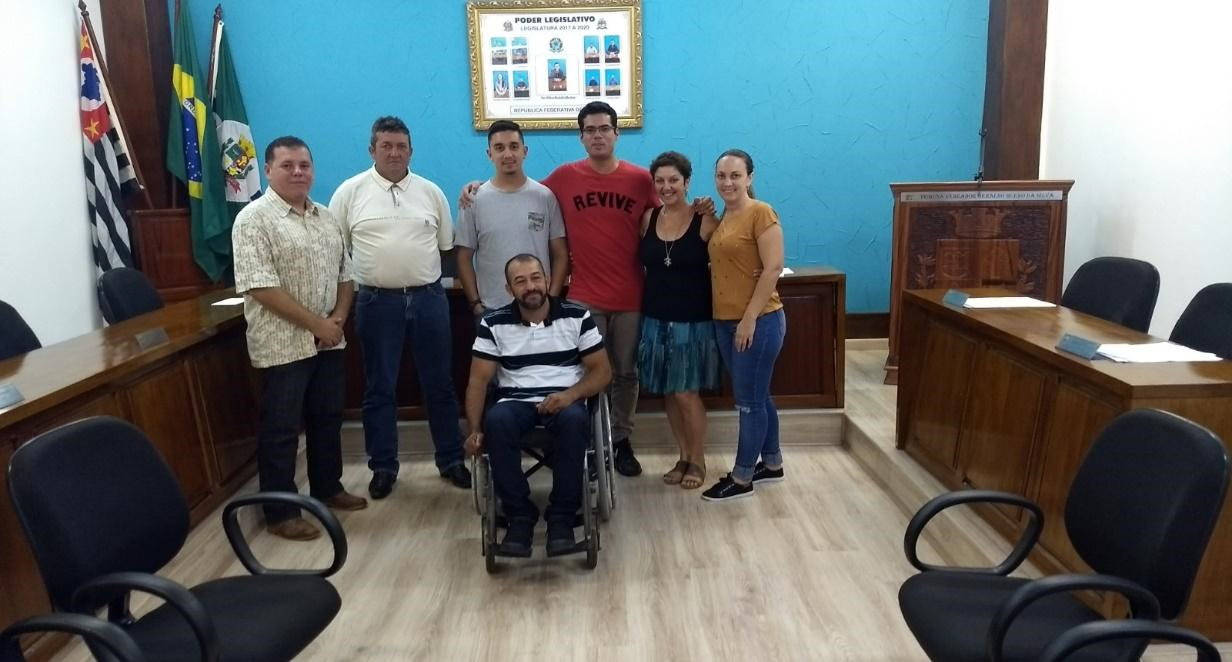
\includegraphics[width=\linewidth]{produtos/produm/danielepub}
	\caption{Encontro do estagiário Daniel com vereadores de Monteiro Lobato e integrantes da secretaria de meio ambiente}
	\label{fig:danielepub}
\end{figure}

O conteúdo das mensagens a serem distribuídas aos moradores, com o intuito de mobilização social, poderão abranger aspectos relacionados à logística dos resíduos (para coleta e para a destinação final), localização e tipo de material a ser usado em novas lixeiras, redução de geração de resíduos, custos do sistema de gestão e possibilidade de redução de custos em função da redução da geração dos resíduos, segurança no manuseio de resíduos, valorização do profissional que atua em contato direto com os resíduos, além da importância de separação dos tipos de resíduos gerados, na fonte geradora, entre inúmeros outros possíveis. Uma vez estabelecido o canal de comunicação com cada morador, poderão ser agendadas audiências públicas, reuniões entre líderes comunitários e representantes políticos, palestras, bem como festivais e eventos culturais para congregação de todos os interessados ou qualquer outra forma de comunicação e diálogo que convier no momento em que ocorrer a necessidade de diálogo e disseminação de informação entre comunidade e equipe responsável pela elaboração e implementação do PMGIRS.

No entanto, ressalta-se que o conteúdo específico a ser divulgado em cada etapa (elaboração, implementação, fiscalização e revisão) deverá ser definido em conjunto com todos os envolvidos e responsáveis pela elaboração do PMGIRS, o que inclui técnicos e servidores municipais. Nesta seção, será enfatizada a forma com que cada tipo de morador de Monteiro Lobato deverá ser abordado. Nesse contexto, as mensagens mobilizadoras deverão ser transmitidas com o intuito de provocar, orientar, mas também incitar o diálogo com a comunidade lobatense (MMA; ICLEI-BRASIL, 2012).

\subsection{Morador tradicional}

Deverá ser mobilizado de duas maneiras:
\begin{itemize}
	\item contato direto e pessoal, de porta em porta;
	\item contato indireto, por meio de igrejas e parcerias com líderes religiosos do município.
\end{itemize}

Na \autoref{fig:estrategmobi}, são apresentadas as etapas a serem seguidas para que se alcance o máximo de participantes de hábitos tradicionais.

\begin{figure}[h!]
	\centering
	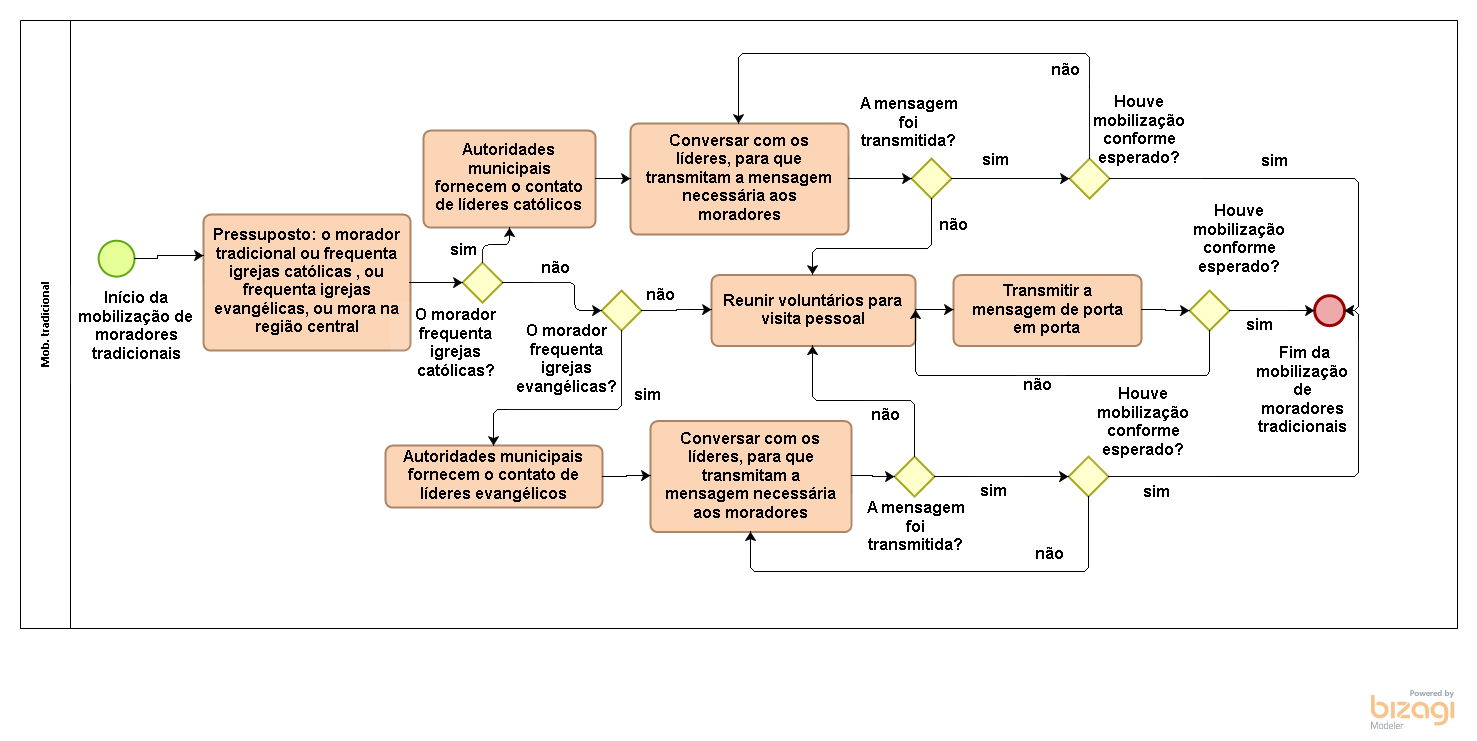
\includegraphics[width=\linewidth]{produtos/produm/estrategmobi}
	\caption{Estratégia de mobilização de moradores tradicionais}
	\label{fig:estrategmobi}
\end{figure}

Poderão ser reunidos como voluntários quaisquer alunos, servidores públicos ou munícipes devidamente treinados para conversar com o morador tradicional. No treinamento, deverão ser definidos:

\begin{itemize}
	\item Vestes a serem usadas;
	\item Linguagem e forma de abordagem;
	\item Conteúdo a ser transmitido;
	\item Tempo de fala;
	\item Conhecimento mínimo sobre o PMGIRS para que o visitante possa responder a eventuais
	perguntas dos moradores.
\end{itemize}

Em entrevista realizada na época de elaboração do plano, na câmara de vereadores de Monteiro Lobato, foi acordado entre vereadores e a secretária de meio ambiente, que os mesmos poderiam contribuir no acesso a líderes religiosos do município.

Deve-se também ressaltar a importância do estimulo fornecido pelo poder publico para que as associações de bairro realizem ações de mobilização mais efetiva da população.

\subsection{Morador de áreas rurais}

A mobilização da comunidade de áreas rurais será mais efetiva, caso as informações sobre a elaboração e implementação do PMGIRS sejam transmitidas por meio de pessoas de sua confiança, tendo como núcleo de ação as escolas rurais de ensino básico. Para que isso aconteça, apresenta-se na \autoref{fig:estrategmobiarearural} a estratégia por meio da qual será alcançada a participação comunitária, em etapas de execução na forma de um fluxograma.

\begin{figure}[h!]
	\centering
	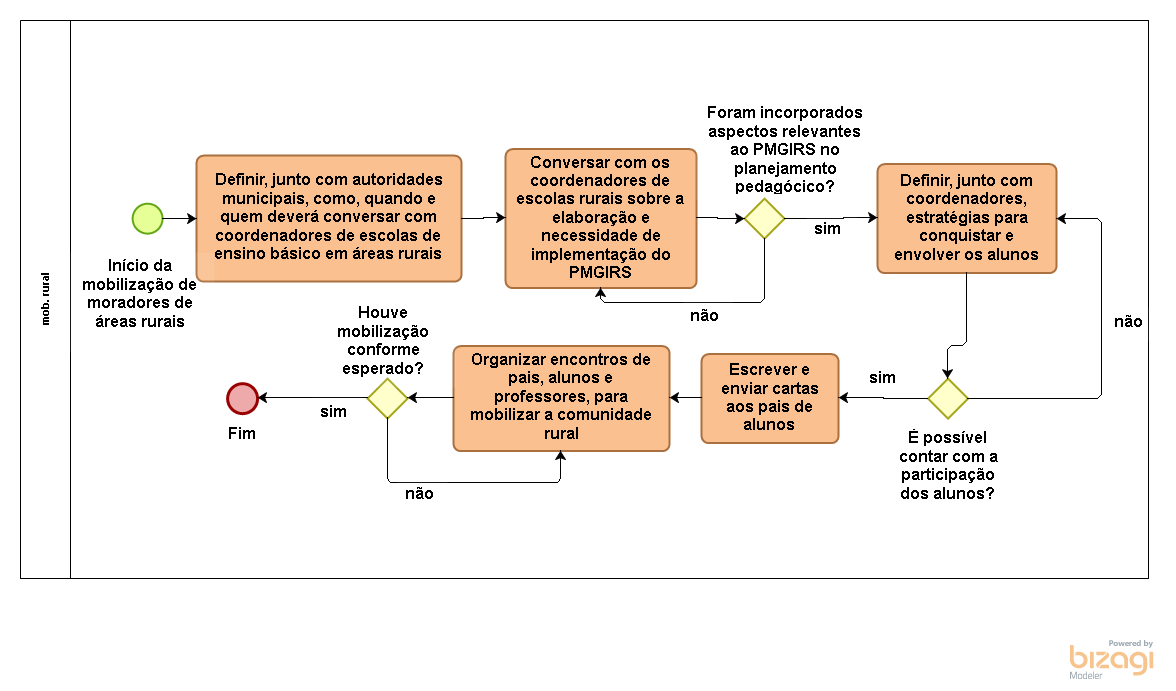
\includegraphics[width=\linewidth]{produtos/produm/estrategmobiarearural}
	\caption{Estratégia de mobilização de moradores de áreas rurais}
	\label{fig:estrategmobiarearural}
\end{figure}

A pessoa encarregada de conversar com os coordenadores de escolas rurais deverá saber se portar, comunicar, e transmitir de forma clara e precisa a necessidade de envolvimento das escolas na elaboração e implementação do PMGIRS. A tarefa poderá ser executada por um aluno estagiário ou não, com ou sem a apresentação de slides. Uma vez alcançado o comprometimento dos coordenadores de escolas e incorporada a temática de planejamento municipal da gestão dos resíduos sólidos no plano pedagógico de ensino, os alunos poderão ser envolvidos por meio de atividades diversas, tais como:
\begin{enumerate}
	\item Gincanas; 
	\item Redações; 
	\item Apresentações sobre o tema durante as aulas; 
	\item Estimulo de redução de consumo; 
	\item Visitas a locais de tratamento de resíduos, tais como um aterro sanitário ou uma cooperativa; 
	\item Mutirões para coleta de resíduos descartados irregularmente na área rural. 
\end{enumerate}

Com o apoio de coordenadores, educadores e alunos, os adultos, pais e familiares de áreas rurais, poderão ser envolvidos com maior facilidade, em encontros, reuniões, eventos escolares, etc. Assim, espera-se que um maior número da comunidade rural participará ou estará ciente de que sua participação é importante para o sucesso do PMGIRS.

\subsection{Turistas e visitantes}
A principal preocupação manifestada por autoridades municipais, em relação à visitação e turismo, refere-se ao respeito à dinâmica de separação dos tipos de resíduos e conservação da limpeza em todas as regiões visitadas, tanto no centro da cidade, como em pousadas mais afastadas do centro.  Além disso, foi ressaltada a importância de colaboração, por parte de todos os transeuntes (visitantes ou não), com as práticas e hábitos a serem implementados no município, em função das ações de implementação do PMGIRS. Assim, tendo como base essas preocupações principais, foi elaborada a estratégia para mobilização de visitantes e turistas, apresentada na \autoref{fig:estrategmobiturista}.

\begin{figure}[h!]
	\centering
	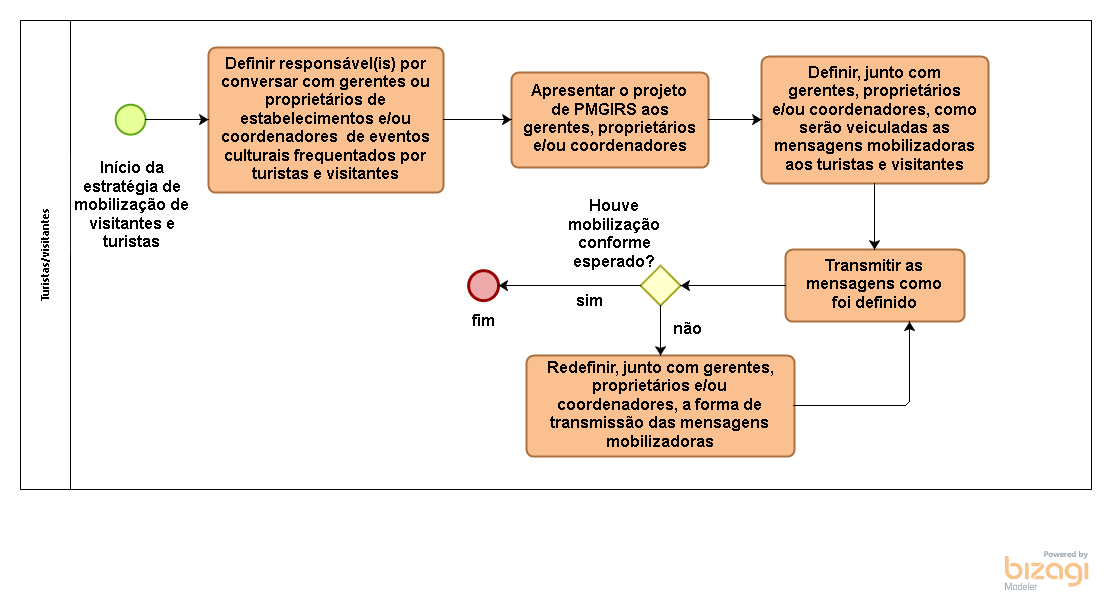
\includegraphics[width=\linewidth]{produtos/produm/estrategmobiturista}
	\caption{Estratégia de mobilização de visitantes e turistas}
	\label{fig:estrategmobiturista}
\end{figure}

Turistas e visitantes não são moradores; mas frequentam restaurantes, pousadas, hotéis e eventos culturais, gerando resíduos e podendo degradar a qualidade ambiental do município. Assim, deverão ser contatados a partir dos locais que frequentam, a partir de diálogo com donos de pousadas, hotéis, restaurantes e, eventualmente, coordenadores de festivais e eventos culturais em que haja aglomeração de pessoas, tais como o carnaval e festas de culinária e personagens de literatura infantil. A partir do diálogo com os gestores de estabelecimentos e locais turísticos, as ações de mobilização com foco nas necessidades de implementação ou elaboração do PMNGIRS deverão ser elaboradas e executadas.


\subsection{Morador jovem}

Como jovem, entende-se o conjunto de moradores com idades entre 15 e 24 anos (IBGE, 2017).  Esse público, deverá ser contatado por meio de estratégias de encontros virtuais, conforme apresentado na \autoref{fig:estrategmobijovem}.

\begin{figure}[h!]
	\centering
	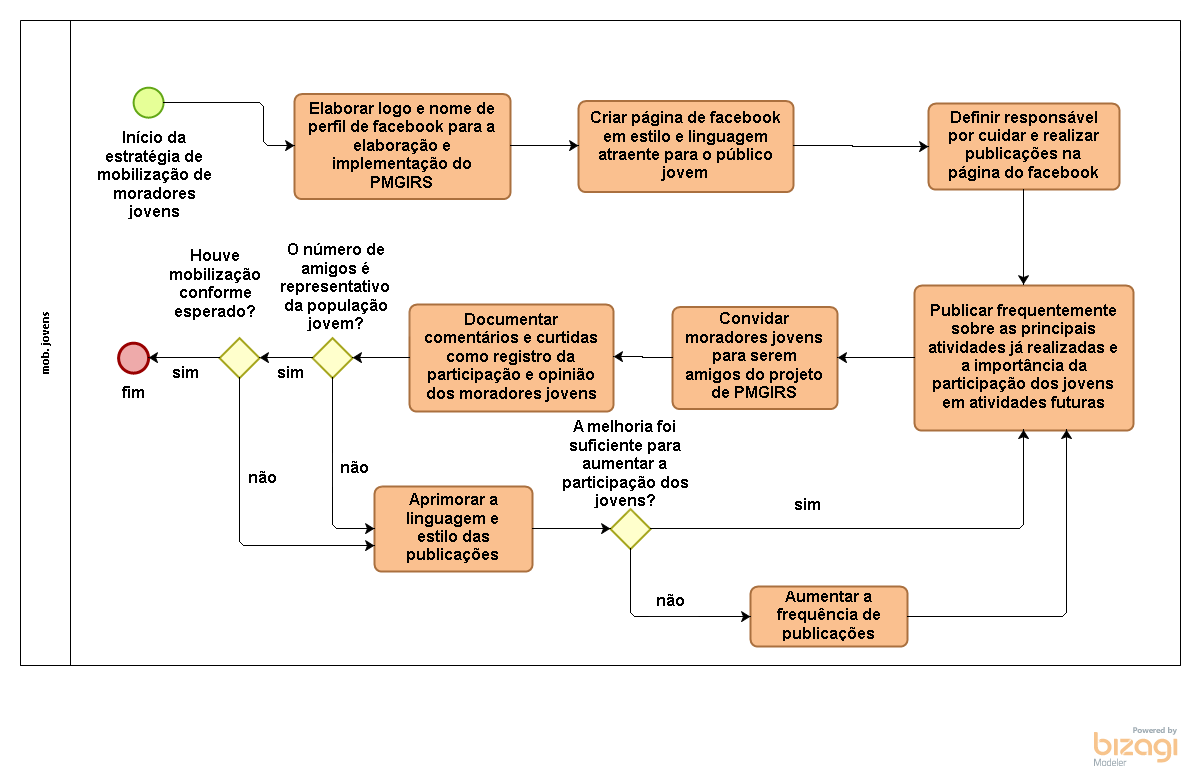
\includegraphics[width=\linewidth]{produtos/produm/estrategmobijovem}
	\caption{Estratégia de mobilização de moradores jovens}
	\label{fig:estrategmobijovem}
\end{figure}

O responsável por cuidar e realizar publicações na página criada do Facebook deverá ser definido em conjunto com autoridades do município e membros da equipe acadêmica responsável pela elaboração do PMGIRS. Sugere-se que a frequência de publicações seja diretamente proporcional à frequência com que novas ações sejam realizadas.

Para saber se o número de indivíduos com acesso à página é representativo ou não, sugere-se a adoção de uma proporção de representatividade a ser definida em conjunto com autoridades municipais. Essa proporção poderá ser, por exemplo, igual ou superior a 70\% da população de jovens do município (IBGE, 2017). Maiores informações sobre amostras significativas estão disponíveis em Bussab e Bolfarine (2005).


\section{Oficina para a apresentação do diagnóstico e discussões acerca da realização do prognóstico}

\subsection{Metodologia}

A oficina participativa é um instrumento amplamente utilizado para aproximar entidades públicas ou privadas de comunidades que são diretamente afetadas por ações, empreendimento ou políticas que possam alterar o cotidiano de uma população. Nessa prática, procura-se informar as condições dos locais que receberão tais ações, os estudos efetuados e resultados obtidos até o momento. A informação é passada de forma simples, direta e transparente cientificando e elucidando as informações à população, quanto ao andamento e às possíveis alterações que ocorrerão dentro de escopo apresentado.

A participação da população nessa etapa é de suma importância para o andamento das ações pretendidas, pois será neste momento que a população terá a possibilidade de fazer críticas/considerações sobre os dados apresentados e sobre as ações propostas, podendo também propor alternativas mais condizentes com as necessidades locais, bem como se informar sobre o andamento das ações.

Em Monteiro Lobato foram efetuadas 4 oficinas participativas (tabela q), de um total de 5 oficinas previstas, nas quais foi explicado aos participantes as condições relacionadas à produção, descarte, transporte e destinação dos resíduos sólidos do município. A estrutura da oficina é baseada em uma metodologia conhecida "Word Café". Esse sistema é um processo participativo com capacidade de trabalhar a diversidade e complexidade no grupo, fazendo emergir a inteligência coletiva. O processo é organizado de forma que as pessoas circulem entre os diversos grupos e conversas, conectando e semeando as ideias, tornando visível a inteligência e a sabedoria do coletivo. A oficina foi dividida em 3 etapas com 20 minutos cada: 

\begin{itemize}
	\item Apresentação dos dados municipais referentes aos resíduos gerados majoritariamente pela população (Resíduo Sólidos Urbano (RSU), Resíduos de Construção Civil (RCC), Resíduos de Serviços de Saúde (RSS) e logística reversa);
	\item Dinâmica inicial em grupo, por classe de resíduo ou conjunto de classes;
	\begin{itemize}
	\item Discussão interna feita pelos participantes sobre problemas relacionados à(s) classe(s) e seus possíveis motivos;
	\item descrição escrita em papéis separados sobre problemas e motivos destes problemas percebidos pela população;
	\item apresentação para todos os participantes das considerações feitas em grupo, seguida de rodas de discussão dos conteúdos apresentados e aprimoramento das ideias.
	\end{itemize}
	\item Dinâmica final em grupo, por classe de resíduo ou conjunto de classe;
	\begin{itemize}
	\item discussão interna sobre possíveis soluções relacionados à(s) classe(s) e como proporcionar seu acontecimento;
	\item descrição escrita em papéis separados sobre possíveis soluções e métodos para sua execução;
	\item apresentação para todos participante das considerações feitas seguida de rodas de discussão dos conteúdos apresentados e aprimoramento das ideias.
	\end{itemize}
\end{itemize}

A formação de grupos será realizada de acordo com os grandes grupos de classificação de resíduo, sendo que deve haver no mínimo dois grupos ou no máximo quatro, a escolha deve ser realizada de acordo com o número de participantes da oficina. Os objetivos principais são: promover a interação em conjunto dos participantes para identificar os principais problemas do município relacionados ao tratamento dos resíduos sólidos no município de Monteiro Lobato. Além disso deve ocorrer uma discussão mais especifica sobre os problemas comuns relacionados aos resíduos a que foram atribuídos ao grupo, bem como as soluções viáveis para mitigar os problemas encontrados e a magnitude dos impactos negativos e positivos, dos problemas e das soluções respectivamente. A etapa final da oficina consiste na troca de informações entre os grupos com apresentação das ideias e uma discussão entre os participantes.

\thispagestyle{headfootimage}
\EndNoToc

\end{document}